\documentclass[10pt]{article}
\usepackage[margin=2cm]{geometry}
\usepackage[T1]{fontenc}
\usepackage[utf8]{inputenc}
\usepackage{lmodern}
\usepackage{booktabs,longtable,graphicx,float,caption,array,xcolor}
\usepackage[hidelinks]{hyperref}
\captionsetup{font=small,labelfont=bf,skip=4pt}
\setlength{\parskip}{5pt}\setlength{\parindent}{0pt}
\setlength{\LTcapwidth}{\textwidth}
\title{Adjoint-DSMC Parameter Study}
\author{Hansel Carmona}
\date{1 October 2026}
\begin{document}
\maketitle
\tableofcontents
\clearpage

\section{Run Settings}\label{sec:runs}
{\scriptsize\setlength{\tabcolsep}{1.6pt}
\begin{longtable}{rllllrrrrlrrr}
\caption{\label{tab:runs}Every optimisation run. The drag reductions are relative to the circle in percent. Own is measured on the run's own seeds, and Unseen is re-measured on 16 held-out seeds at 250k particles. The pass-4 run took 10 endgame steps after its 30 normal iterations, and its own-seed value is relative to its starting shape rather than the circle.}\\
\toprule
Pass & Run & N\_REF & N\_AVG & N\_FOURIER & \shortstack{GRAD\_INIT\\\_FRAC} & N\_ITER & SEED0 & \shortstack{Iterations\\done} & \shortstack{Stopped\\at} & Own \% & Unseen \% & Hours \\
\midrule
\endfirsthead
\toprule
Pass & Run & N\_REF & N\_AVG & N\_FOURIER & \shortstack{GRAD\_INIT\\\_FRAC} & N\_ITER & SEED0 & \shortstack{Iterations\\done} & \shortstack{Stopped\\at} & Own \% & Unseen \% & Hours \\
\midrule
\endhead
\bottomrule
\endfoot
1 & \texttt{B0\_seed0} & 250k & 4 & 10 & 0.05 & 20 & 0 & 20 & it.\ limit & 51.9 & 51.8 & 0.6 \\
1 & \texttt{nseeds1} & 250k & 1 & 10 & 0.05 & 20 & 0 & 20 & it.\ limit & 50.8 & 51.0 & 0.5 \\
1 & \texttt{nseeds16} & 250k & 16 & 10 & 0.05 & 20 & 0 & 20 & it.\ limit & 51.4 & 51.5 & 0.8 \\
1 & \texttt{nseeds2} & 250k & 2 & 10 & 0.05 & 20 & 0 & 20 & it.\ limit & 52.1 & 52.0 & 0.6 \\
1 & \texttt{nseeds8} & 250k & 8 & 10 & 0.05 & 20 & 0 & 20 & it.\ limit & 51.9 & 51.7 & 0.6 \\
1 & \texttt{nref100k} & 100k & 4 & 10 & 0.05 & 20 & 0 & 20 & it.\ limit & 49.7 & 50.2 & 0.2 \\
1 & \texttt{nref1M} & 1M & 4 & 10 & 0.05 & 20 & 0 & 20 & it.\ limit & 51.1 & 51.1 & 1.8 \\
1 & \texttt{nref500k} & 500k & 4 & 10 & 0.05 & 20 & 0 & 20 & it.\ limit & 52.6 & 52.8 & 0.9 \\
1 & \texttt{nf20} & 250k & 4 & 20 & 0.05 & 20 & 0 & 3 & noise limit & 10.2 & -- & 0.2 \\
1 & \texttt{nf3} & 250k & 4 & 3 & 0.05 & 20 & 0 & 11 & noise limit & 32.4 & 32.6 & 0.3 \\
1 & \texttt{nf5} & 250k & 4 & 5 & 0.05 & 20 & 0 & 20 & it.\ limit & 49.2 & 49.0 & 0.4 \\
1 & \texttt{frac0.01} & 250k & 4 & 10 & 0.01 & 20 & 0 & 20 & it.\ limit & 51.2 & 51.5 & 0.6 \\
1 & \texttt{frac0.02} & 250k & 4 & 10 & 0.02 & 20 & 0 & 20 & it.\ limit & 52.6 & 52.4 & 0.6 \\
1 & \texttt{frac0.1} & 250k & 4 & 10 & 0.1 & 20 & 0 & 20 & it.\ limit & 52.4 & 52.6 & 0.7 \\
1 & \texttt{frac0.2} & 250k & 4 & 10 & 0.2 & 20 & 0 & 20 & it.\ limit & 53.8 & 53.5 & 0.6 \\
2 & \texttt{B0\_seed0} & 250k & 4 & 10 & 0.05 & 50 & 0 & 50 & it.\ limit & 61.8 & 62.0 & 1.6 \\
2 & \texttt{B0\_seed100} & 250k & 4 & 10 & 0.05 & 50 & 100 & 32 & noise limit & 57.9 & 58.3 & 1.1 \\
2 & \texttt{B0\_seed200} & 250k & 4 & 10 & 0.05 & 50 & 200 & 27 & noise limit & 55.0 & 55.4 & 0.9 \\
2 & \texttt{nseeds1\_seed0} & 250k & 1 & 10 & 0.05 & 50 & 0 & 31 & noise limit & 54.4 & 53.7 & 0.9 \\
2 & \texttt{nseeds1\_seed100} & 250k & 1 & 10 & 0.05 & 50 & 100 & 35 & noise limit & 50.5 & 51.2 & 1.0 \\
2 & \texttt{nseeds1\_seed200} & 250k & 1 & 10 & 0.05 & 50 & 200 & 24 & noise limit & 51.4 & 50.4 & 0.8 \\
2 & \texttt{nseeds8\_seed0} & 250k & 8 & 10 & 0.05 & 50 & 0 & 47 & noise limit & 61.2 & 61.4 & 1.5 \\
2 & \texttt{nseeds8\_seed100} & 250k & 8 & 10 & 0.05 & 50 & 100 & 50 & it.\ limit & 62.9 & 62.9 & 1.5 \\
2 & \texttt{nseeds8\_seed200} & 250k & 8 & 10 & 0.05 & 50 & 200 & 50 & it.\ limit & 61.7 & 62.2 & 1.7 \\
2 & \texttt{nref500k\_seed0} & 500k & 4 & 10 & 0.05 & 50 & 0 & 50 & it.\ limit & 62.3 & 62.7 & 2.7 \\
2 & \texttt{nref500k\_seed100} & 500k & 4 & 10 & 0.05 & 50 & 100 & 50 & it.\ limit & 62.5 & 62.7 & 2.8 \\
2 & \texttt{nref500k\_seed200} & 500k & 4 & 10 & 0.05 & 50 & 200 & 50 & it.\ limit & 61.8 & 62.3 & 2.8 \\
2 & \texttt{nf5\_seed0} & 250k & 4 & 5 & 0.05 & 50 & 0 & 22 & noise limit & 49.7 & 49.4 & 0.6 \\
2 & \texttt{nf5\_seed100} & 250k & 4 & 5 & 0.05 & 50 & 100 & 20 & noise limit & 48.8 & 49.5 & 0.4 \\
2 & \texttt{nf5\_seed200} & 250k & 4 & 5 & 0.05 & 50 & 200 & 22 & noise limit & 48.9 & 49.6 & 0.4 \\
2 & \texttt{frac0.1\_seed0} & 250k & 4 & 10 & 0.1 & 50 & 0 & 42 & noise limit & 60.2 & 60.1 & 1.3 \\
2 & \texttt{frac0.1\_seed100} & 250k & 4 & 10 & 0.1 & 50 & 100 & 39 & noise limit & 60.7 & 60.4 & 1.2 \\
2 & \texttt{frac0.1\_seed200} & 250k & 4 & 10 & 0.1 & 50 & 200 & 39 & noise limit & 59.7 & 59.6 & 1.2 \\
3 & \texttt{grow4to32\_seed0} & 250k & 4$\to$32 & 10 & 0.05 & 100 & 0 & 81 & noise limit & 68.5 & 68.1 & 4.1 \\
3 & \texttt{grow4to32\_seed100} & 250k & 4$\to$32 & 10 & 0.05 & 100 & 100 & 100 & it.\ limit & 68.7 & 69.0 & 11.6 \\
3 & \texttt{grow4to32\_seed200} & 250k & 4$\to$32 & 10 & 0.05 & 100 & 200 & 88 & noise limit & 68.4 & 68.6 & 6.1 \\
3 & \texttt{grow4to32\_seed300} & 250k & 4$\to$32 & 10 & 0.05 & 100 & 300 & 100 & it.\ limit & 68.7 & 68.5 & 8.3 \\
4 & \texttt{C3\_1M\_endgame\_seed400} & 1M & 16$\to$32 & 10 & 0.01 & 30+10 & 400 & 20 & noise limit & 0.4 & 68.9 & 6.3 \\
\end{longtable}}


\clearpage\section{Summary figures}\label{sec:figs}
\subsection{Pass 1}
\begin{figure}[H]\centering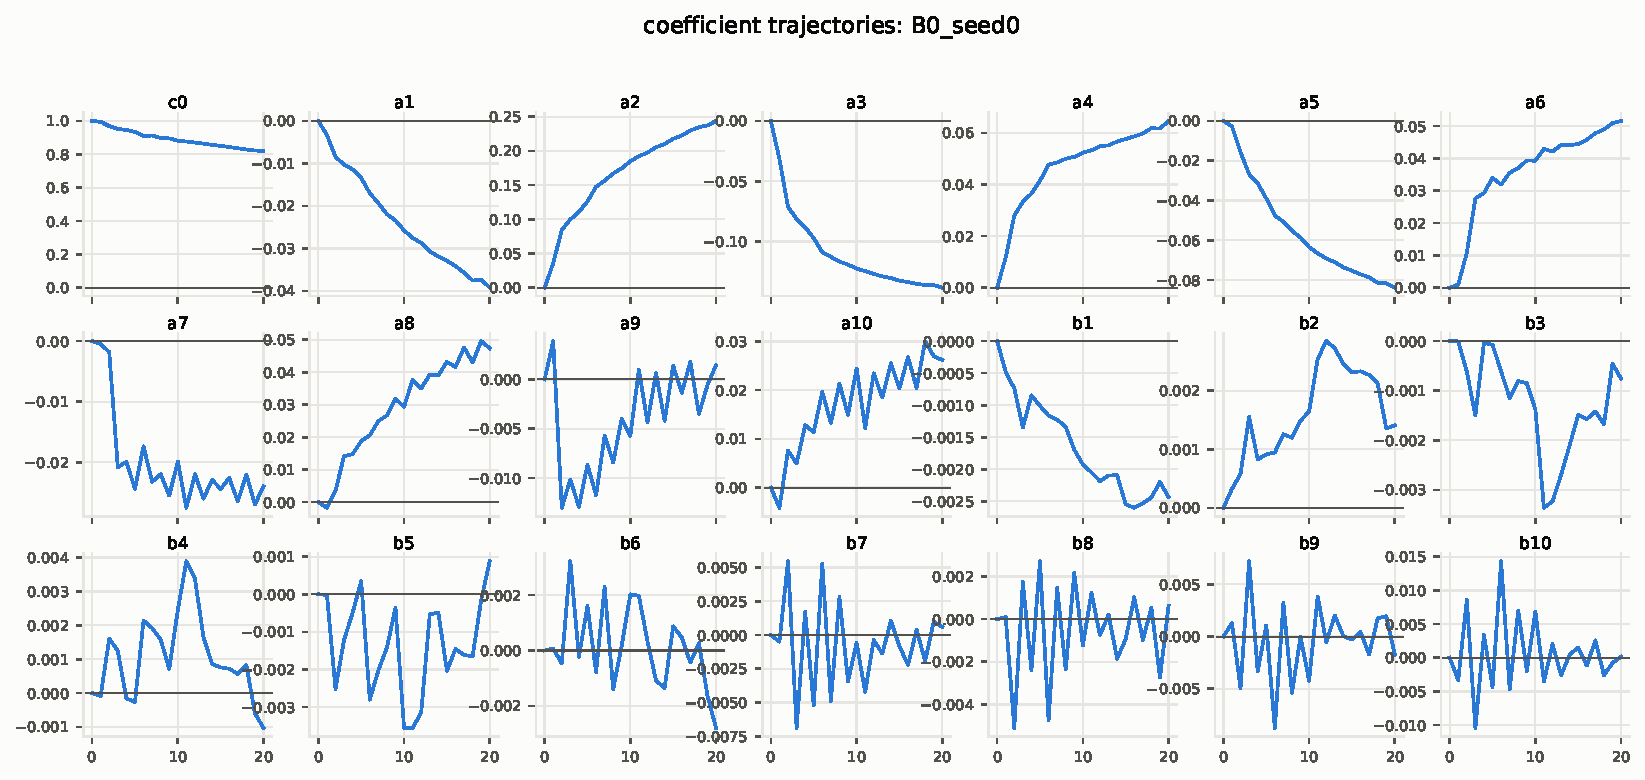
\includegraphics[width=0.92\textwidth,height=0.40\textheight,keepaspectratio]{summary/pass1_coeff_trajectories_B0_seed0.pdf}\caption{This figure shows each Fourier coefficient of the baseline run with SEED0 = 0 against iteration. Pass 1 used N\_REF = 250k, N\_AVG = 4, N\_FOURIER = 10, GRAD\_INIT\_FRAC = 0.05, N\_ITER = 20 and SEED0 = 0, except for the parameter that the figure varies.}\end{figure}
\begin{figure}[H]\centering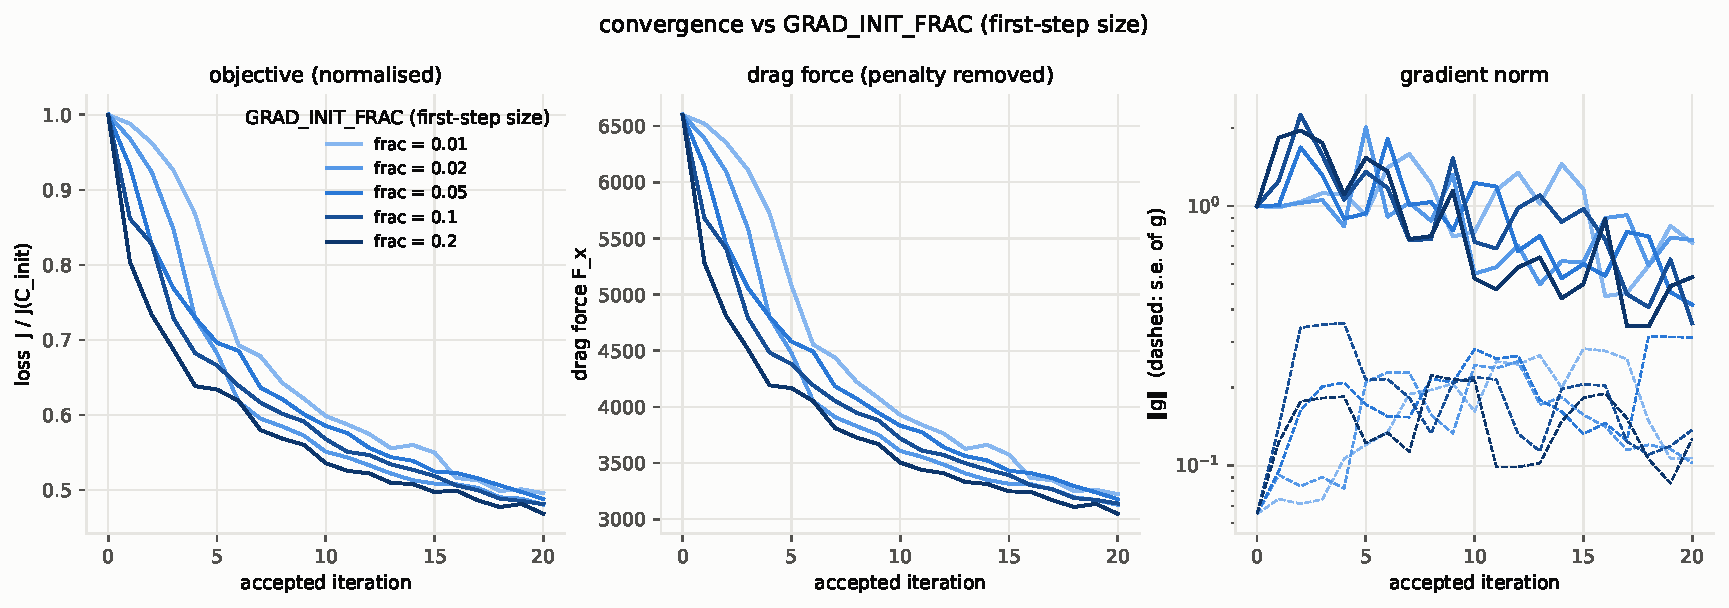
\includegraphics[width=0.92\textwidth,height=0.40\textheight,keepaspectratio]{summary/pass1_convergence_vs_frac.pdf}\caption{This figure shows the objective and the gradient norm against iteration. The runs differ only in GRAD\_INIT\_FRAC. Pass 1 used N\_REF = 250k, N\_AVG = 4, N\_FOURIER = 10, GRAD\_INIT\_FRAC = 0.05, N\_ITER = 20 and SEED0 = 0, except for the parameter that the figure varies.}\end{figure}
\begin{figure}[H]\centering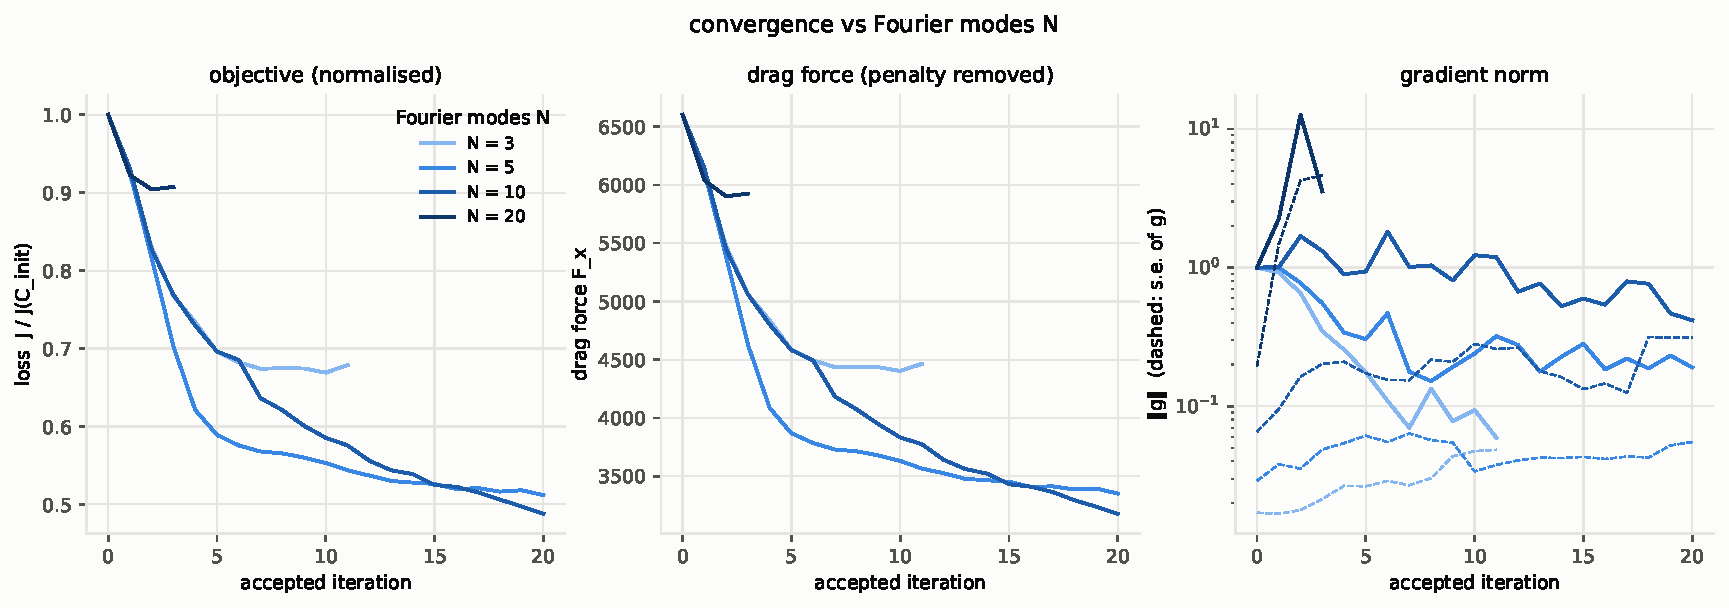
\includegraphics[width=0.92\textwidth,height=0.40\textheight,keepaspectratio]{summary/pass1_convergence_vs_nfourier.pdf}\caption{This figure shows the objective and the gradient norm against iteration. The runs differ only in N\_FOURIER. Pass 1 used N\_REF = 250k, N\_AVG = 4, N\_FOURIER = 10, GRAD\_INIT\_FRAC = 0.05, N\_ITER = 20 and SEED0 = 0, except for the parameter that the figure varies.}\end{figure}
\begin{figure}[H]\centering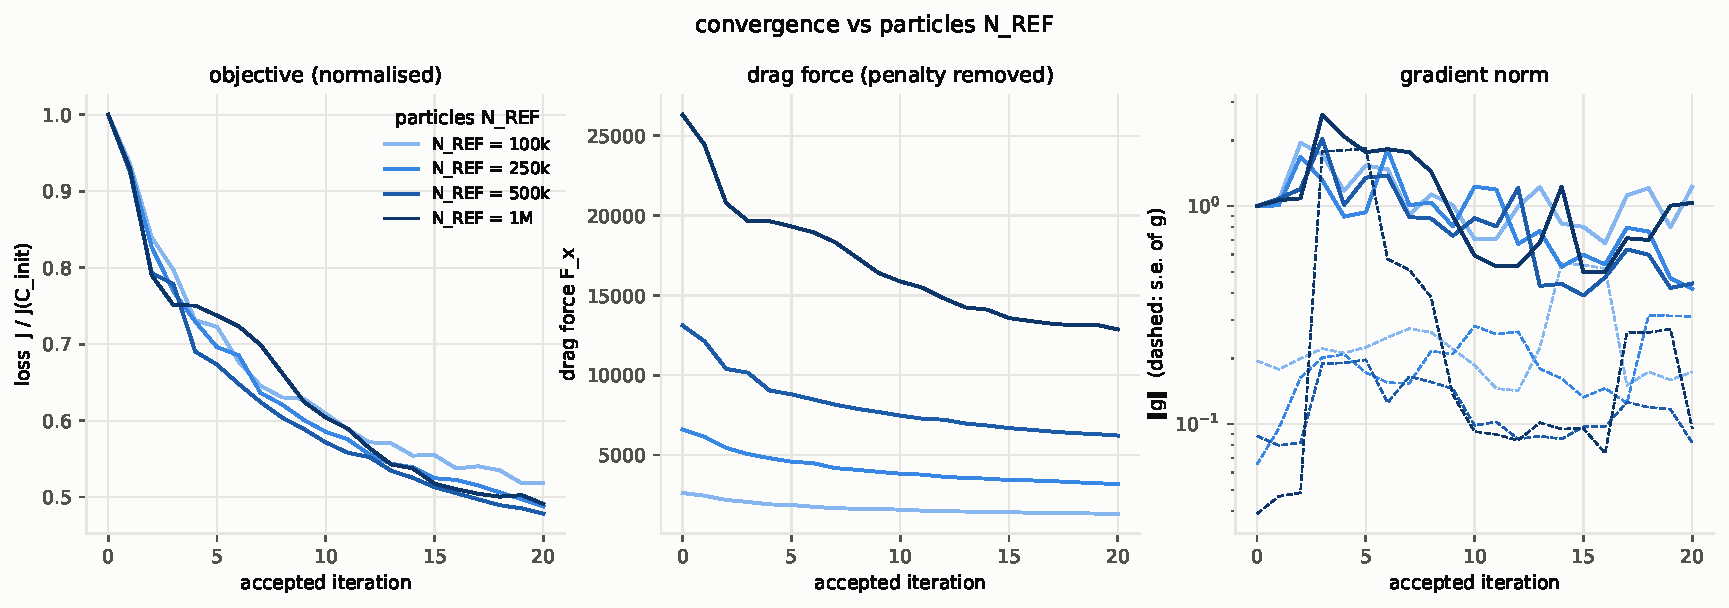
\includegraphics[width=0.92\textwidth,height=0.40\textheight,keepaspectratio]{summary/pass1_convergence_vs_nref.pdf}\caption{This figure shows the objective and the gradient norm against iteration. The runs differ only in N\_REF. Pass 1 used N\_REF = 250k, N\_AVG = 4, N\_FOURIER = 10, GRAD\_INIT\_FRAC = 0.05, N\_ITER = 20 and SEED0 = 0, except for the parameter that the figure varies.}\end{figure}
\begin{figure}[H]\centering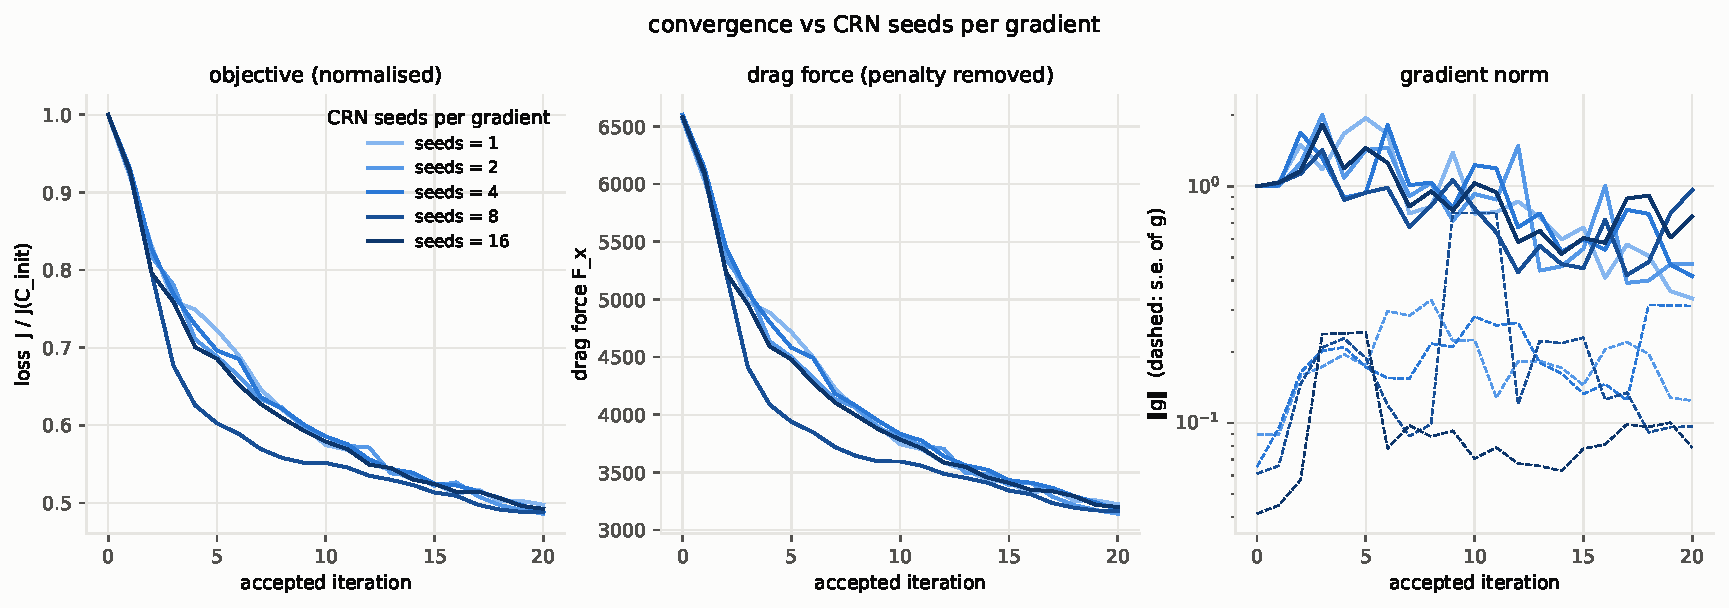
\includegraphics[width=0.92\textwidth,height=0.40\textheight,keepaspectratio]{summary/pass1_convergence_vs_seeds.pdf}\caption{This figure shows the objective and the gradient norm against iteration. The runs differ only in N\_AVG. Pass 1 used N\_REF = 250k, N\_AVG = 4, N\_FOURIER = 10, GRAD\_INIT\_FRAC = 0.05, N\_ITER = 20 and SEED0 = 0, except for the parameter that the figure varies.}\end{figure}
\begin{figure}[H]\centering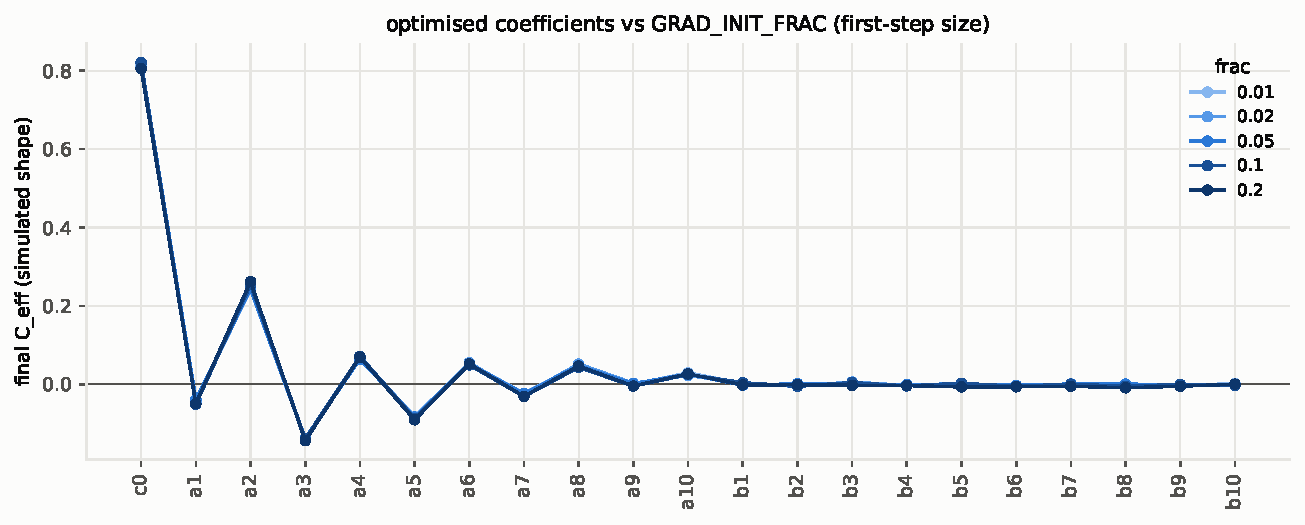
\includegraphics[width=0.92\textwidth,height=0.40\textheight,keepaspectratio]{summary/pass1_final_coeffs_vs_frac.pdf}\caption{This figure shows the final shape coefficients against GRAD\_INIT\_FRAC. Pass 1 used N\_REF = 250k, N\_AVG = 4, N\_FOURIER = 10, GRAD\_INIT\_FRAC = 0.05, N\_ITER = 20 and SEED0 = 0, except for the parameter that the figure varies.}\end{figure}
\begin{figure}[H]\centering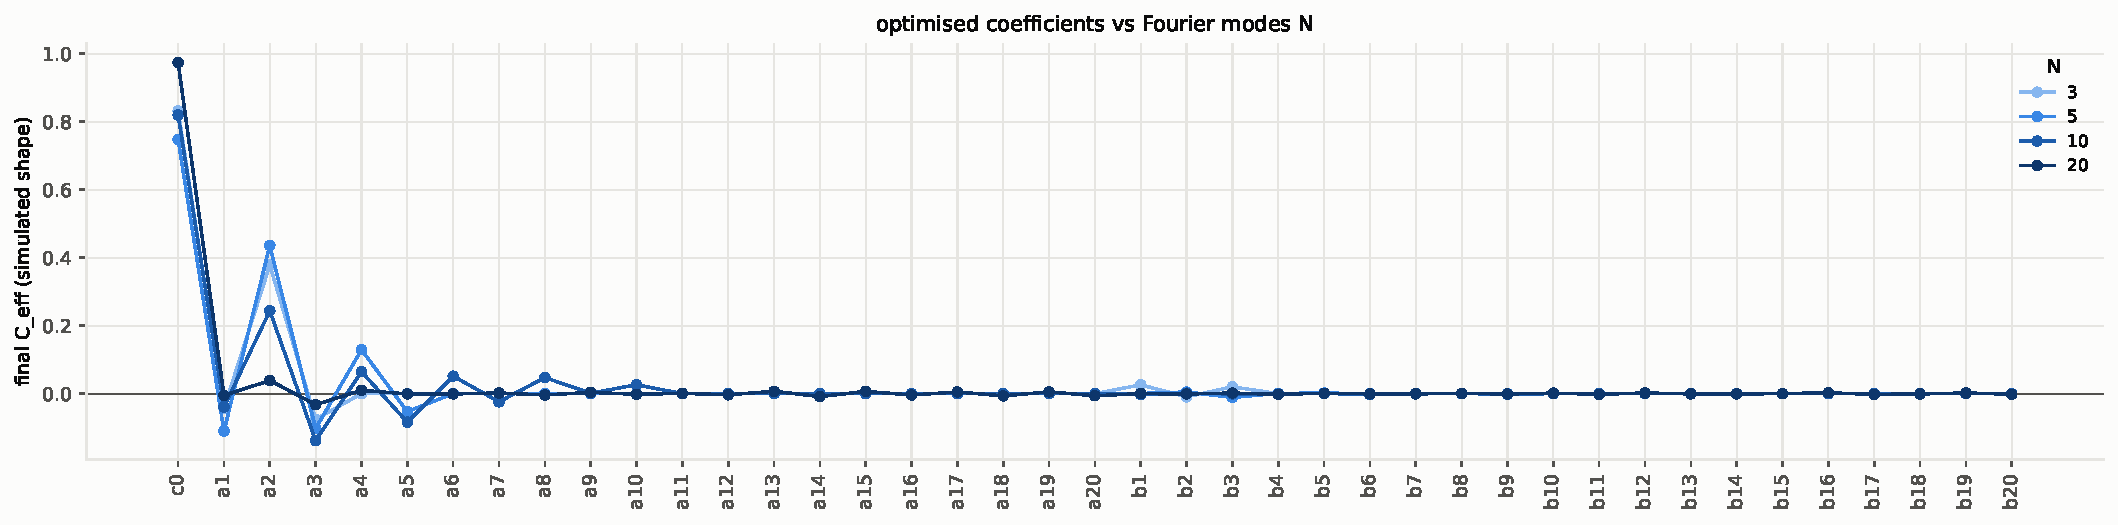
\includegraphics[width=0.92\textwidth,height=0.40\textheight,keepaspectratio]{summary/pass1_final_coeffs_vs_nfourier.pdf}\caption{This figure shows the final shape coefficients against N\_FOURIER. Pass 1 used N\_REF = 250k, N\_AVG = 4, N\_FOURIER = 10, GRAD\_INIT\_FRAC = 0.05, N\_ITER = 20 and SEED0 = 0, except for the parameter that the figure varies.}\end{figure}
\begin{figure}[H]\centering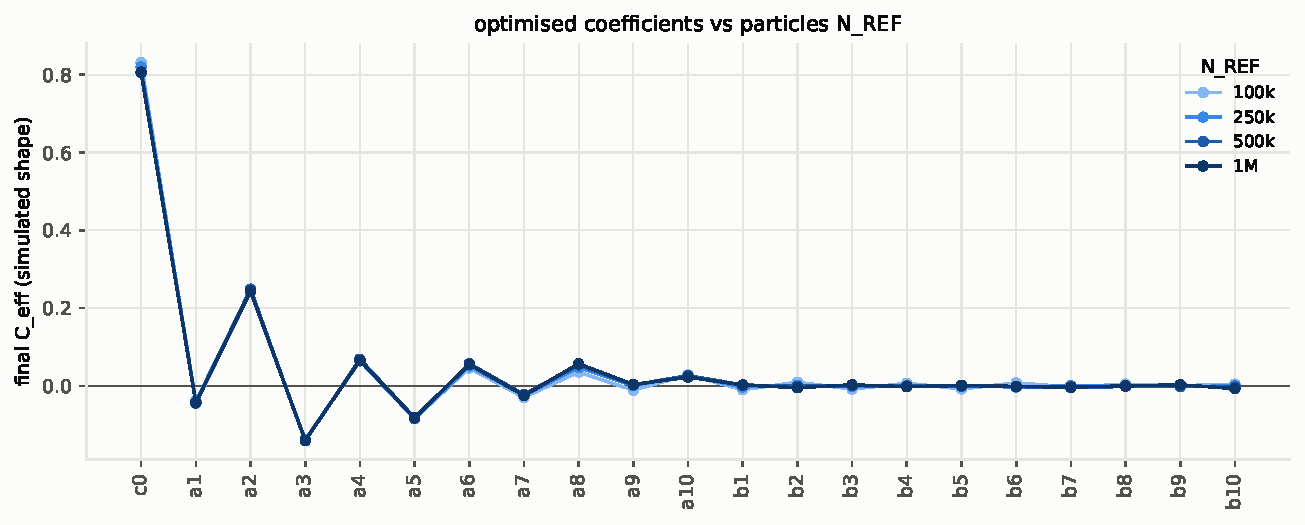
\includegraphics[width=0.92\textwidth,height=0.40\textheight,keepaspectratio]{summary/pass1_final_coeffs_vs_nref.pdf}\caption{This figure shows the final shape coefficients against N\_REF. Pass 1 used N\_REF = 250k, N\_AVG = 4, N\_FOURIER = 10, GRAD\_INIT\_FRAC = 0.05, N\_ITER = 20 and SEED0 = 0, except for the parameter that the figure varies.}\end{figure}
\begin{figure}[H]\centering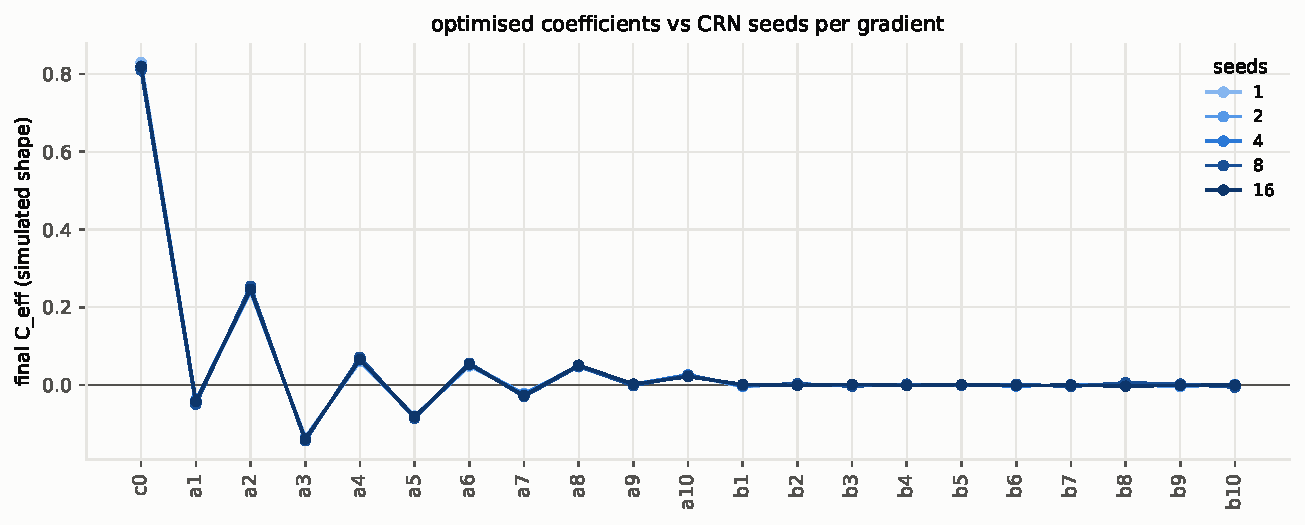
\includegraphics[width=0.92\textwidth,height=0.40\textheight,keepaspectratio]{summary/pass1_final_coeffs_vs_seeds.pdf}\caption{This figure shows the final shape coefficients against N\_AVG. Pass 1 used N\_REF = 250k, N\_AVG = 4, N\_FOURIER = 10, GRAD\_INIT\_FRAC = 0.05, N\_ITER = 20 and SEED0 = 0, except for the parameter that the figure varies.}\end{figure}
\begin{figure}[H]\centering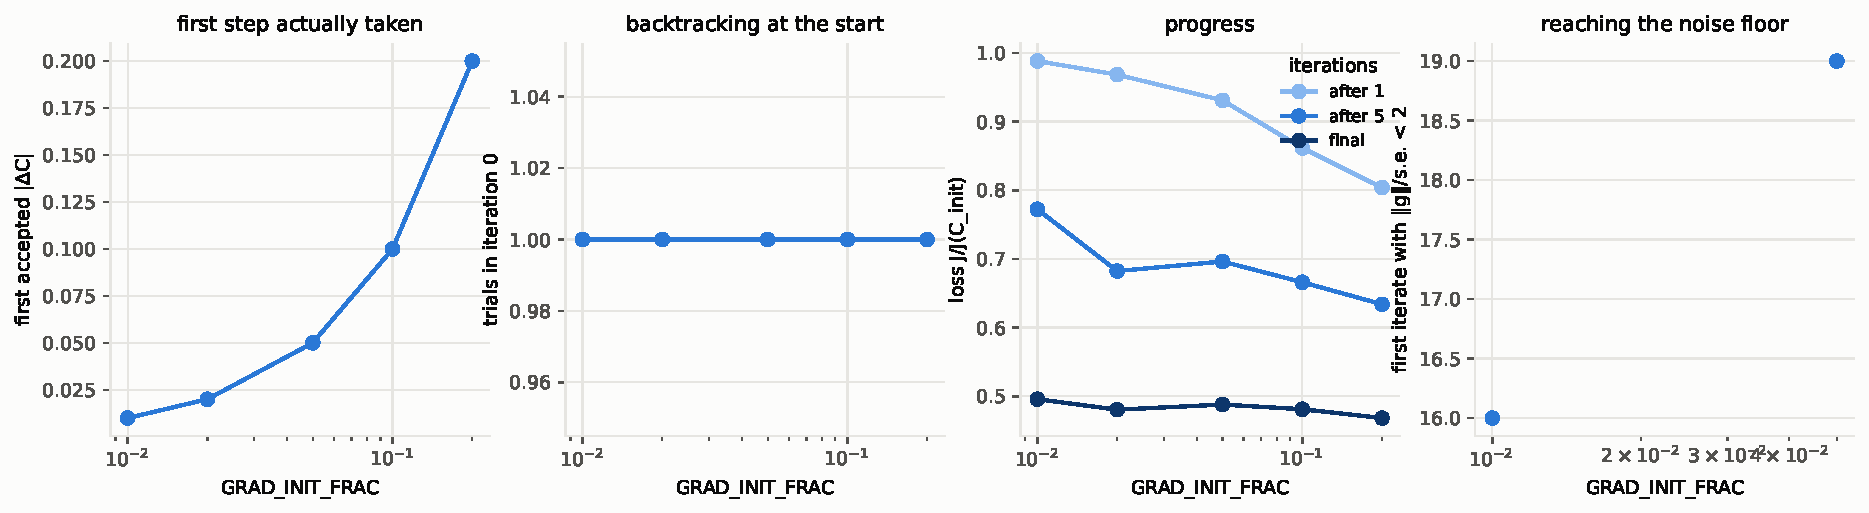
\includegraphics[width=0.92\textwidth,height=0.40\textheight,keepaspectratio]{summary/pass1_grad_init_frac_effects.pdf}\caption{This figure shows how the first-step size affects the first accepted step, the number of backtracks at iteration 0, and the objective after 1, 5 and 20 iterations. Pass 1 used N\_REF = 250k, N\_AVG = 4, N\_FOURIER = 10, GRAD\_INIT\_FRAC = 0.05, N\_ITER = 20 and SEED0 = 0, except for the parameter that the figure varies.}\end{figure}
\begin{figure}[H]\centering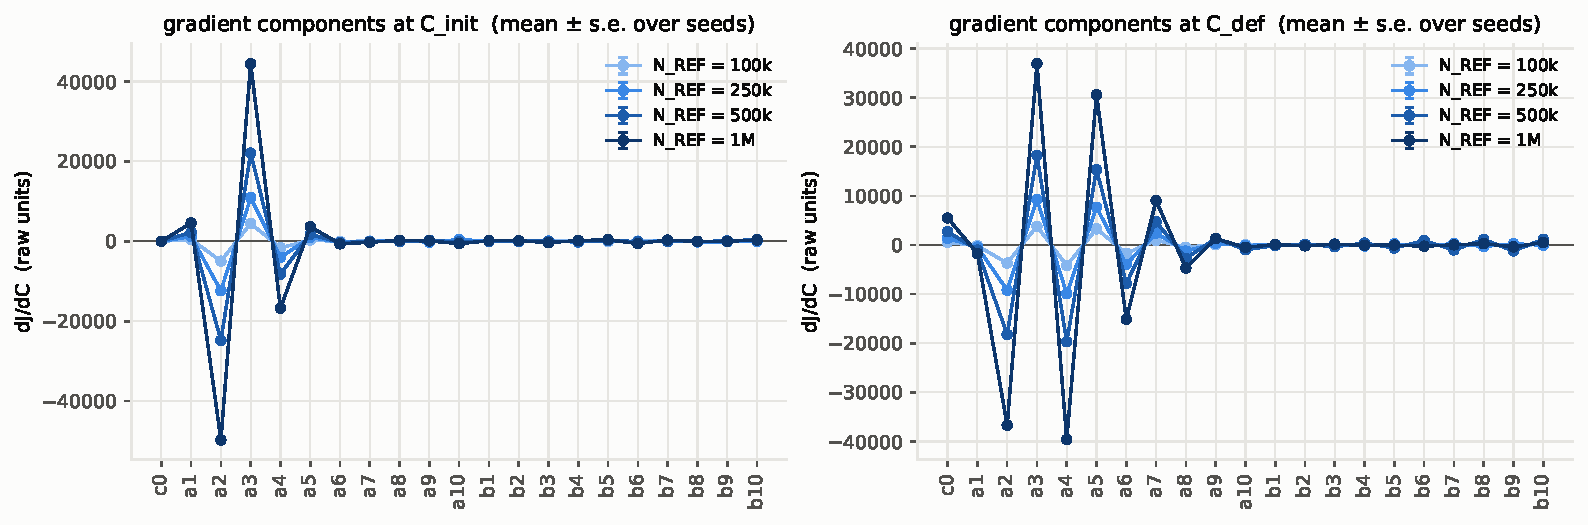
\includegraphics[width=0.92\textwidth,height=0.40\textheight,keepaspectratio]{summary/pass1_grad_mean_vs_nref.pdf}\caption{This figure shows the mean gradient of each mode, with its standard error over 16 seeds, against the particle count at the circle and at the stretched shape ($a_2 = 0.15$). Pass 1 used N\_REF = 250k, N\_AVG = 4, N\_FOURIER = 10, GRAD\_INIT\_FRAC = 0.05, N\_ITER = 20 and SEED0 = 0, except for the parameter that the figure varies.}\end{figure}
\begin{figure}[H]\centering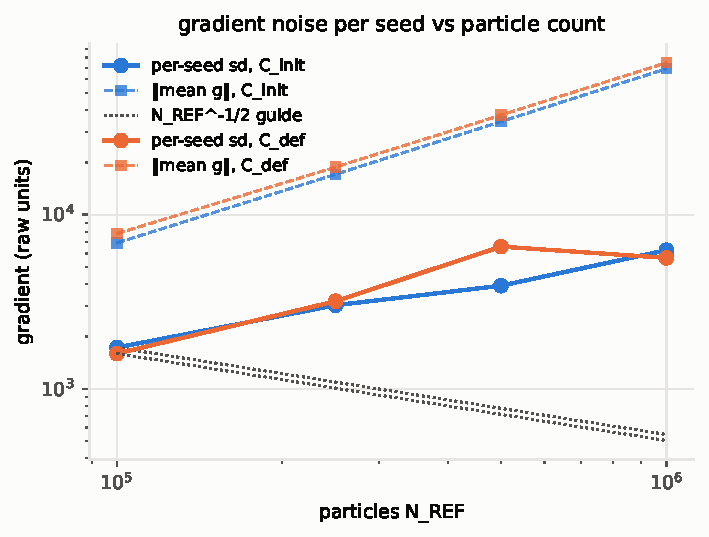
\includegraphics[width=0.92\textwidth,height=0.40\textheight,keepaspectratio]{summary/pass1_grad_sd_vs_nref.pdf}\caption{This figure shows the scatter of one seed's gradient against the particle count on logarithmic axes, with an $N^{-1/2}$ guide. Pass 1 used N\_REF = 250k, N\_AVG = 4, N\_FOURIER = 10, GRAD\_INIT\_FRAC = 0.05, N\_ITER = 20 and SEED0 = 0, except for the parameter that the figure varies.}\end{figure}
\begin{figure}[H]\centering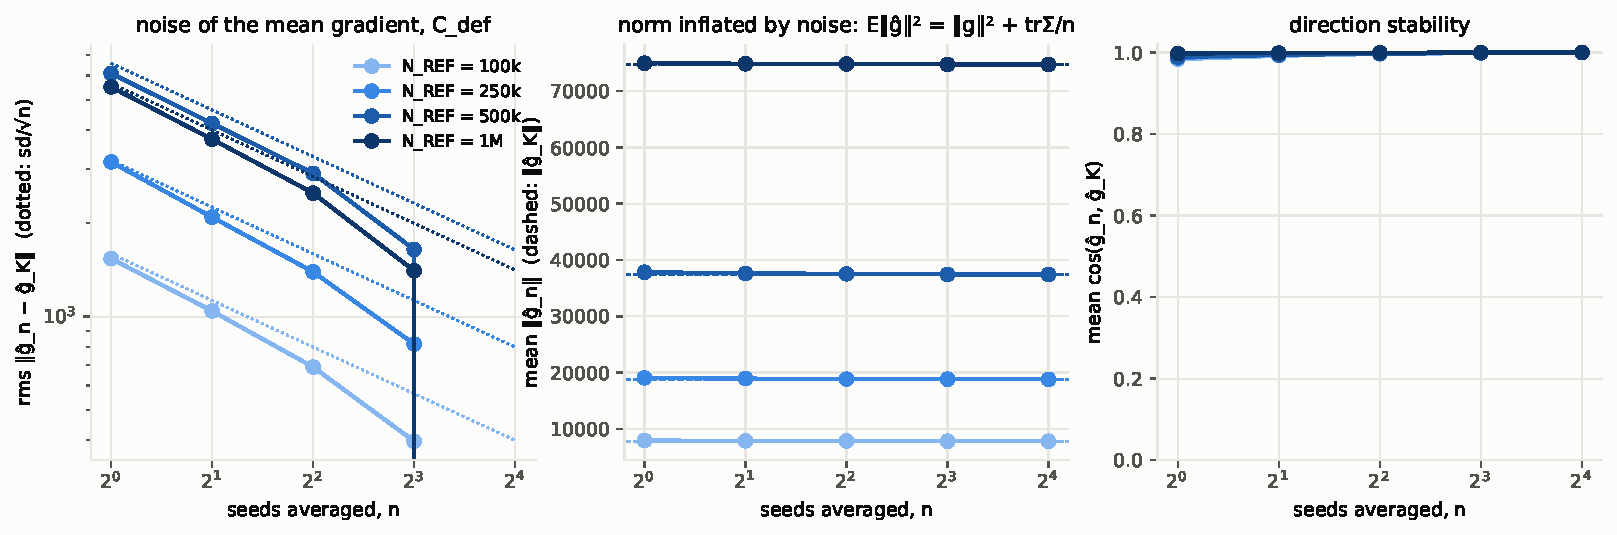
\includegraphics[width=0.92\textwidth,height=0.40\textheight,keepaspectratio]{summary/pass1_grad_se_vs_nseeds_C_def.pdf}\caption{This figure shows the error of an $n$-seed average against $n$ at the stretched shape ($a_2 = 0.15$), together with the $1/\sqrt{n}$ prediction. Pass 1 used N\_REF = 250k, N\_AVG = 4, N\_FOURIER = 10, GRAD\_INIT\_FRAC = 0.05, N\_ITER = 20 and SEED0 = 0, except for the parameter that the figure varies.}\end{figure}
\begin{figure}[H]\centering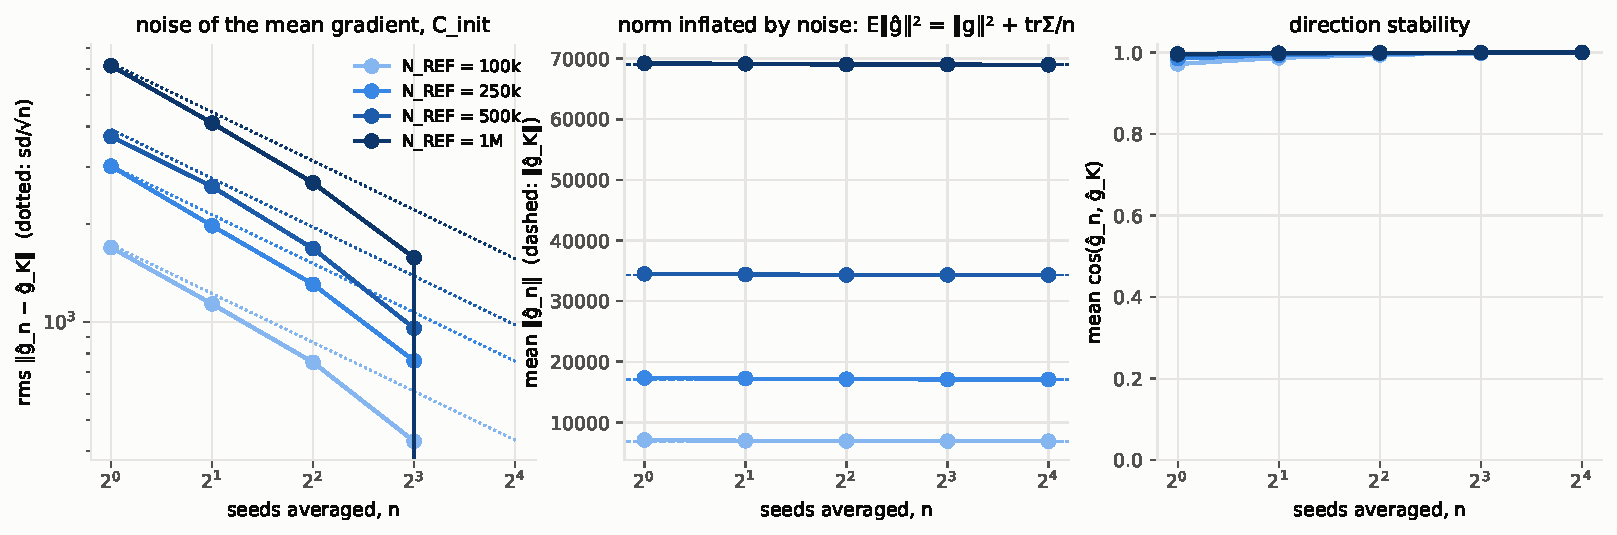
\includegraphics[width=0.92\textwidth,height=0.40\textheight,keepaspectratio]{summary/pass1_grad_se_vs_nseeds_C_init.pdf}\caption{This figure shows the error of an $n$-seed average against $n$ at the circle, together with the $1/\sqrt{n}$ prediction. Pass 1 used N\_REF = 250k, N\_AVG = 4, N\_FOURIER = 10, GRAD\_INIT\_FRAC = 0.05, N\_ITER = 20 and SEED0 = 0, except for the parameter that the figure varies.}\end{figure}
\begin{figure}[H]\centering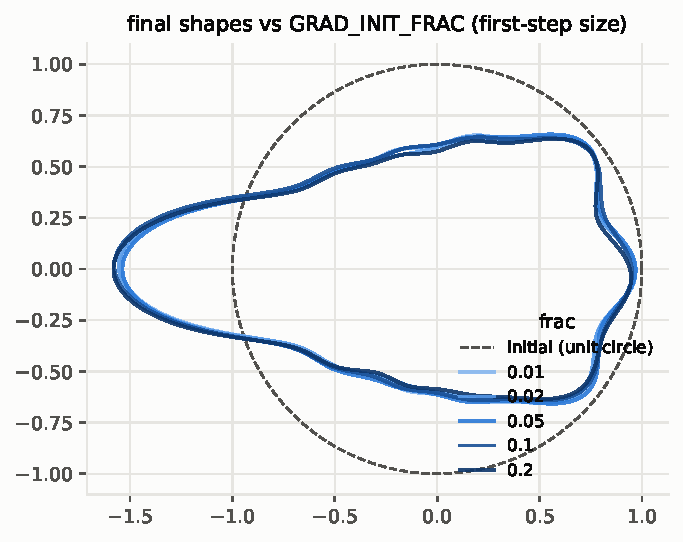
\includegraphics[width=0.92\textwidth,height=0.40\textheight,keepaspectratio]{summary/pass1_shapes_vs_frac.pdf}\caption{This figure shows the final shapes for each value of GRAD\_INIT\_FRAC. Pass 1 used N\_REF = 250k, N\_AVG = 4, N\_FOURIER = 10, GRAD\_INIT\_FRAC = 0.05, N\_ITER = 20 and SEED0 = 0, except for the parameter that the figure varies.}\end{figure}
\begin{figure}[H]\centering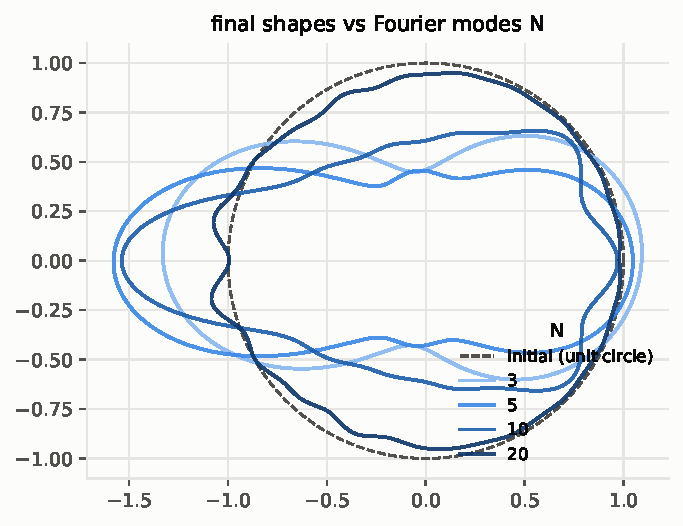
\includegraphics[width=0.92\textwidth,height=0.40\textheight,keepaspectratio]{summary/pass1_shapes_vs_nfourier.pdf}\caption{This figure shows the final shapes for each value of N\_FOURIER. Pass 1 used N\_REF = 250k, N\_AVG = 4, N\_FOURIER = 10, GRAD\_INIT\_FRAC = 0.05, N\_ITER = 20 and SEED0 = 0, except for the parameter that the figure varies.}\end{figure}
\begin{figure}[H]\centering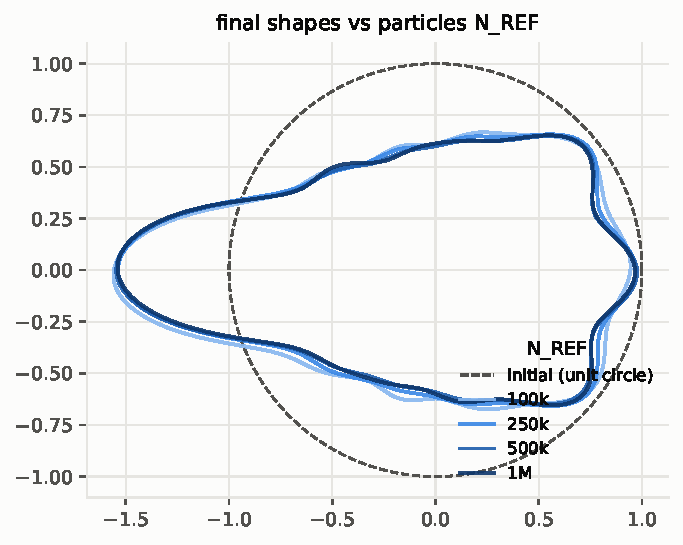
\includegraphics[width=0.92\textwidth,height=0.40\textheight,keepaspectratio]{summary/pass1_shapes_vs_nref.pdf}\caption{This figure shows the final shapes for each value of N\_REF. Pass 1 used N\_REF = 250k, N\_AVG = 4, N\_FOURIER = 10, GRAD\_INIT\_FRAC = 0.05, N\_ITER = 20 and SEED0 = 0, except for the parameter that the figure varies.}\end{figure}
\begin{figure}[H]\centering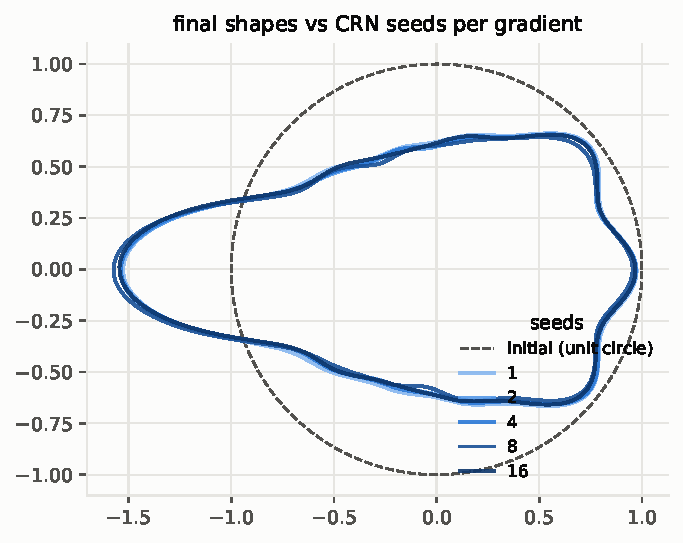
\includegraphics[width=0.92\textwidth,height=0.40\textheight,keepaspectratio]{summary/pass1_shapes_vs_seeds.pdf}\caption{This figure shows the final shapes for each value of N\_AVG. Pass 1 used N\_REF = 250k, N\_AVG = 4, N\_FOURIER = 10, GRAD\_INIT\_FRAC = 0.05, N\_ITER = 20 and SEED0 = 0, except for the parameter that the figure varies.}\end{figure}
\begin{figure}[H]\centering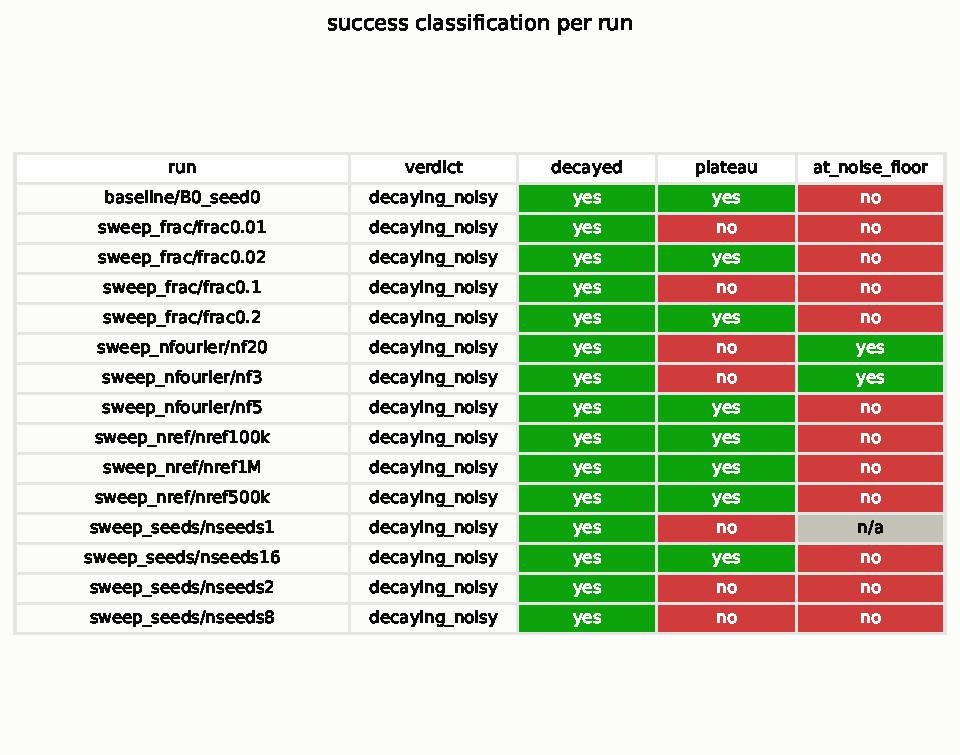
\includegraphics[width=0.92\textwidth,height=0.40\textheight,keepaspectratio]{summary/pass1_success_table.pdf}\caption{This figure shows the automatic classifier's verdict for each run. For 1-seed runs a success verdict is an artefact, because a single seed gives no noise estimate. Pass 1 used N\_REF = 250k, N\_AVG = 4, N\_FOURIER = 10, GRAD\_INIT\_FRAC = 0.05, N\_ITER = 20 and SEED0 = 0, except for the parameter that the figure varies.}\end{figure}
\begin{figure}[H]\centering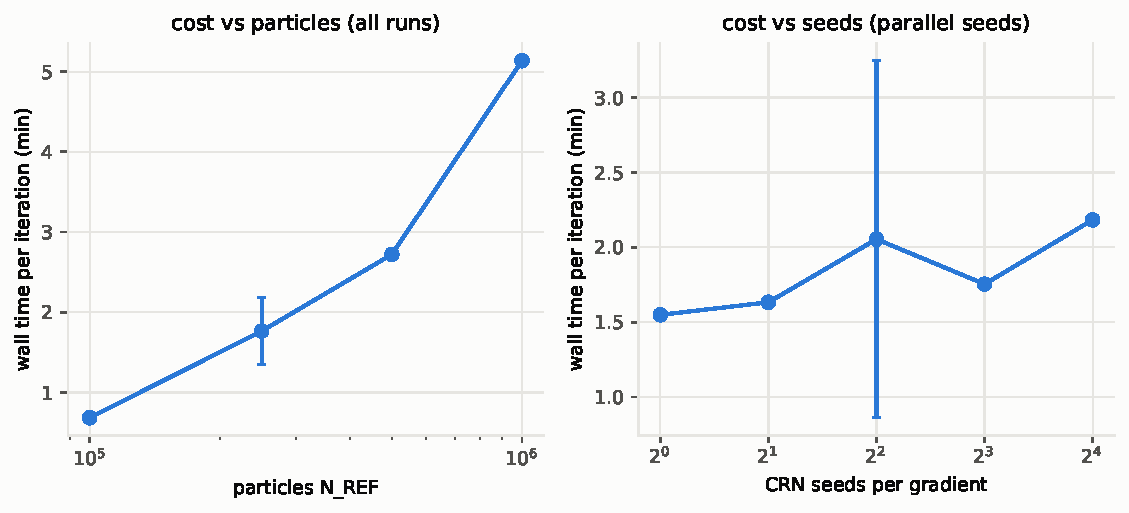
\includegraphics[width=0.92\textwidth,height=0.40\textheight,keepaspectratio]{summary/pass1_wall_per_iter.pdf}\caption{This figure shows the wall-clock time per iteration against the particle count and the number of seeds. Pass 1 used N\_REF = 250k, N\_AVG = 4, N\_FOURIER = 10, GRAD\_INIT\_FRAC = 0.05, N\_ITER = 20 and SEED0 = 0, except for the parameter that the figure varies.}\end{figure}
\subsection{Pass 2}
\begin{figure}[H]\centering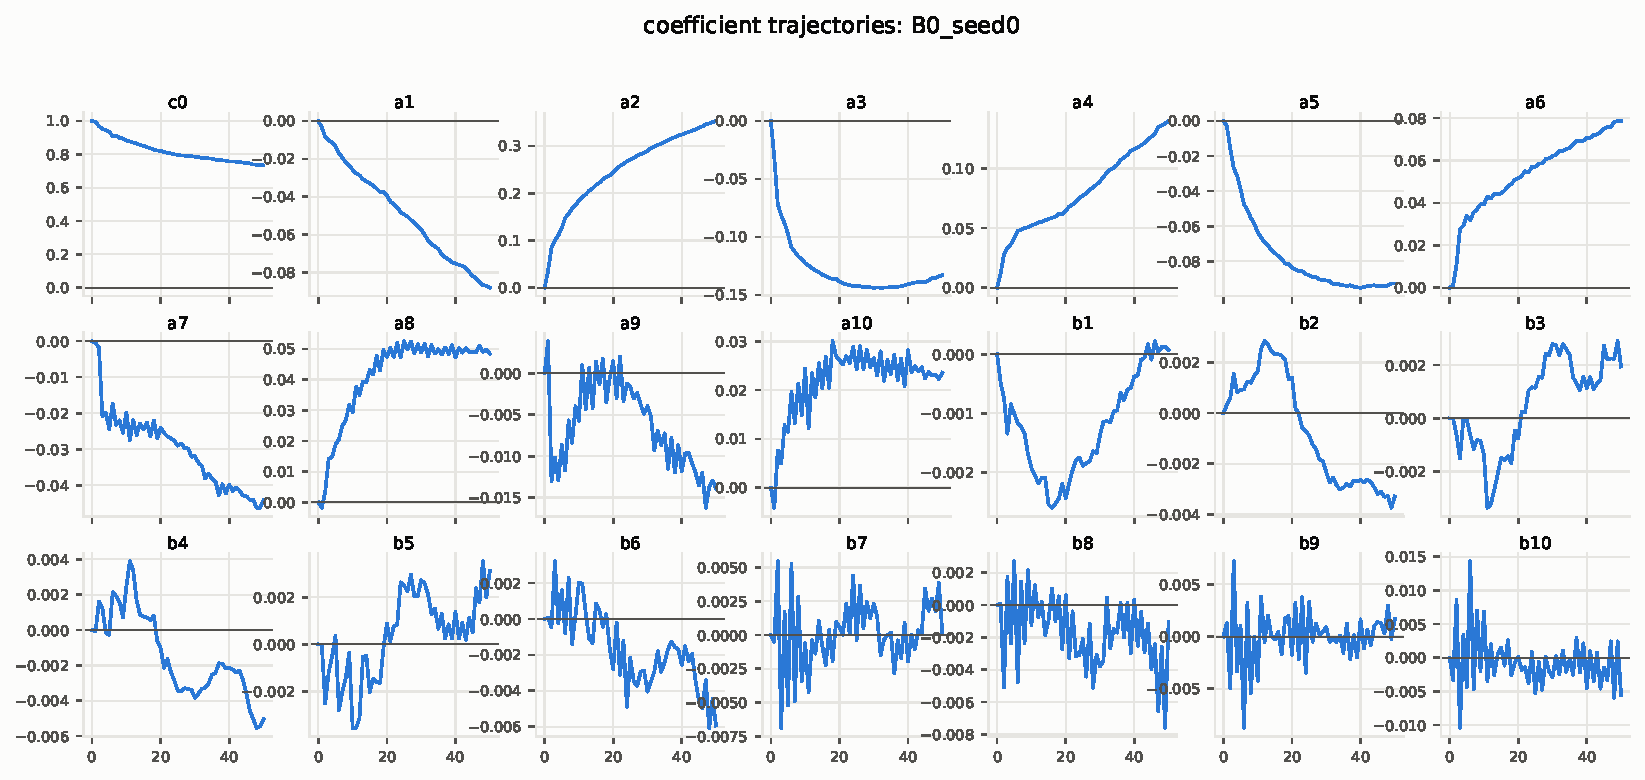
\includegraphics[width=0.92\textwidth,height=0.40\textheight,keepaspectratio]{summary/pass2_coeff_trajectories_B0_seed0.pdf}\caption{This figure shows each Fourier coefficient of the baseline run with SEED0 = 0 against iteration. Pass 2 used the same settings with N\_ITER = 50 and SEED0 = 0, 100 and 200.}\end{figure}
\begin{figure}[H]\centering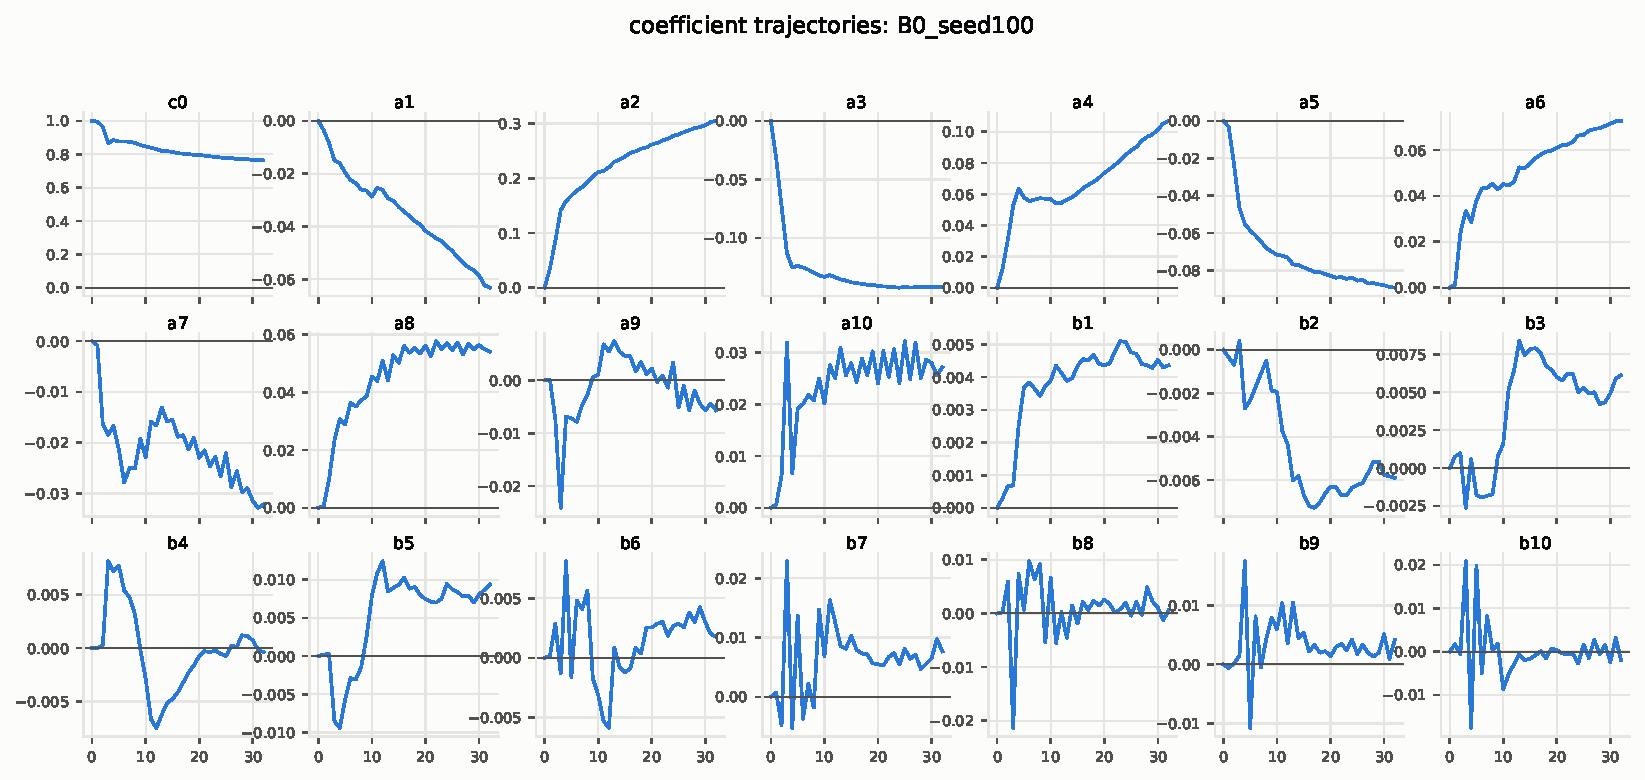
\includegraphics[width=0.92\textwidth,height=0.40\textheight,keepaspectratio]{summary/pass2_coeff_trajectories_B0_seed100.pdf}\caption{This figure shows each Fourier coefficient of the baseline run with SEED0 = 100 against iteration. Pass 2 used the same settings with N\_ITER = 50 and SEED0 = 0, 100 and 200.}\end{figure}
\begin{figure}[H]\centering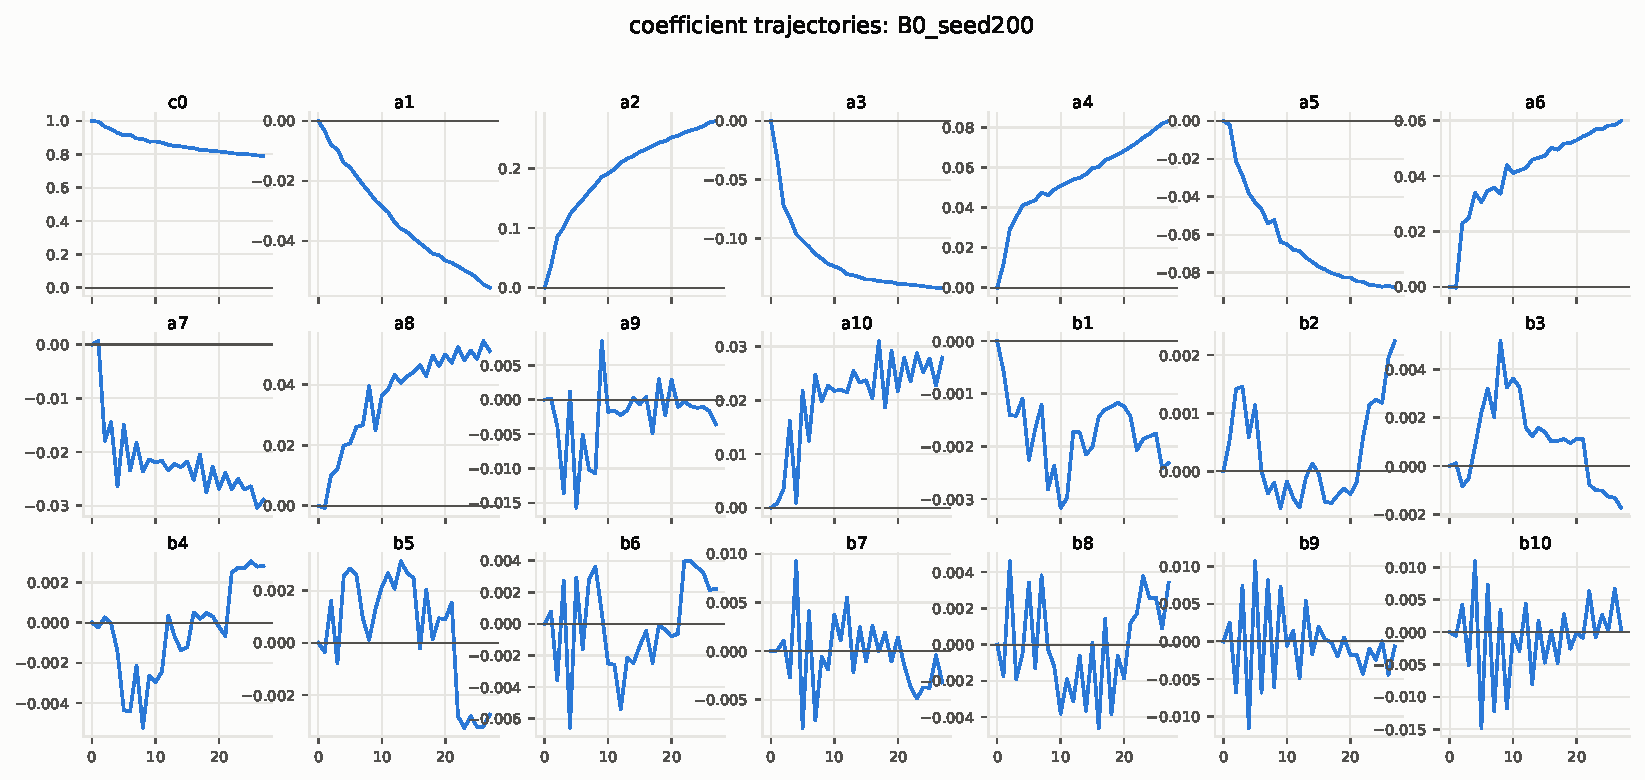
\includegraphics[width=0.92\textwidth,height=0.40\textheight,keepaspectratio]{summary/pass2_coeff_trajectories_B0_seed200.pdf}\caption{This figure shows each Fourier coefficient of the baseline run with SEED0 = 200 against iteration. Pass 2 used the same settings with N\_ITER = 50 and SEED0 = 0, 100 and 200.}\end{figure}
\begin{figure}[H]\centering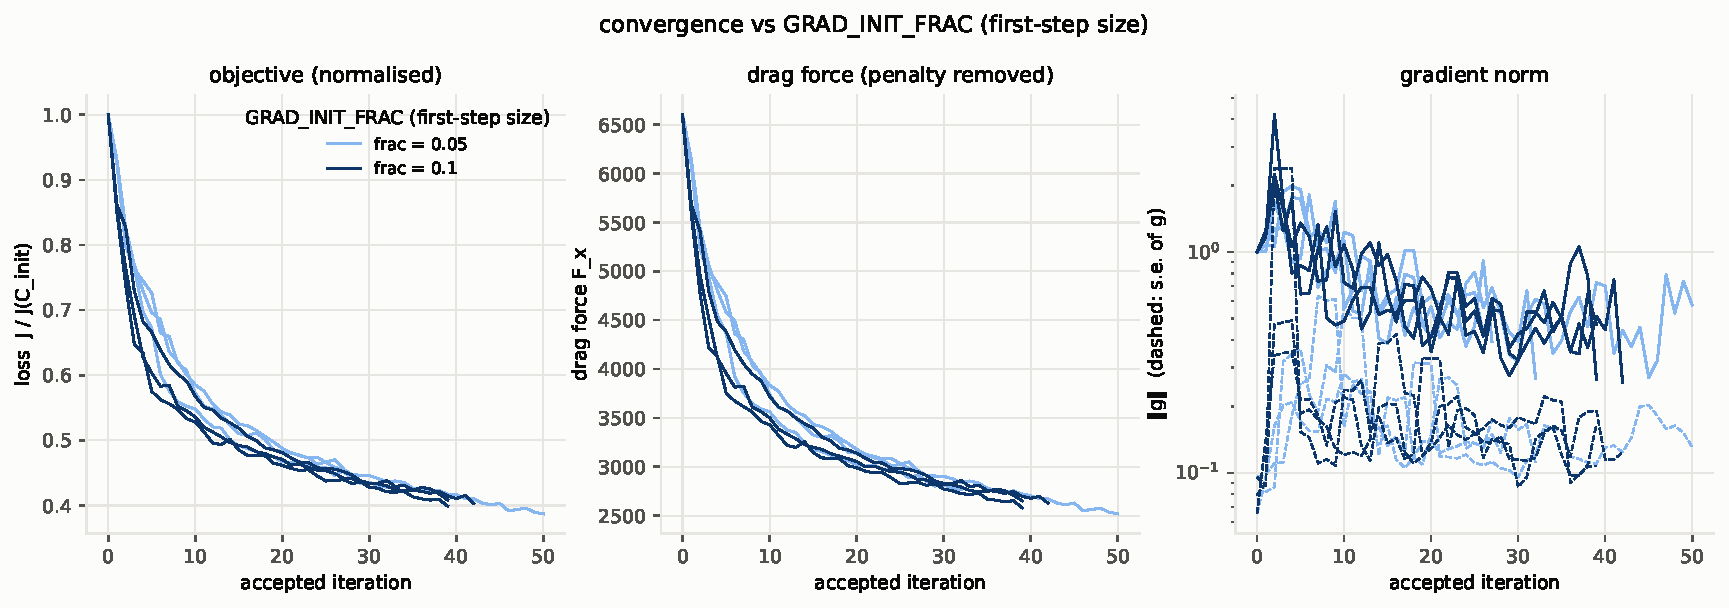
\includegraphics[width=0.92\textwidth,height=0.40\textheight,keepaspectratio]{summary/pass2_convergence_vs_frac.pdf}\caption{This figure shows the objective and the gradient norm against iteration. The runs differ only in GRAD\_INIT\_FRAC. Pass 2 used the same settings with N\_ITER = 50 and SEED0 = 0, 100 and 200.}\end{figure}
\begin{figure}[H]\centering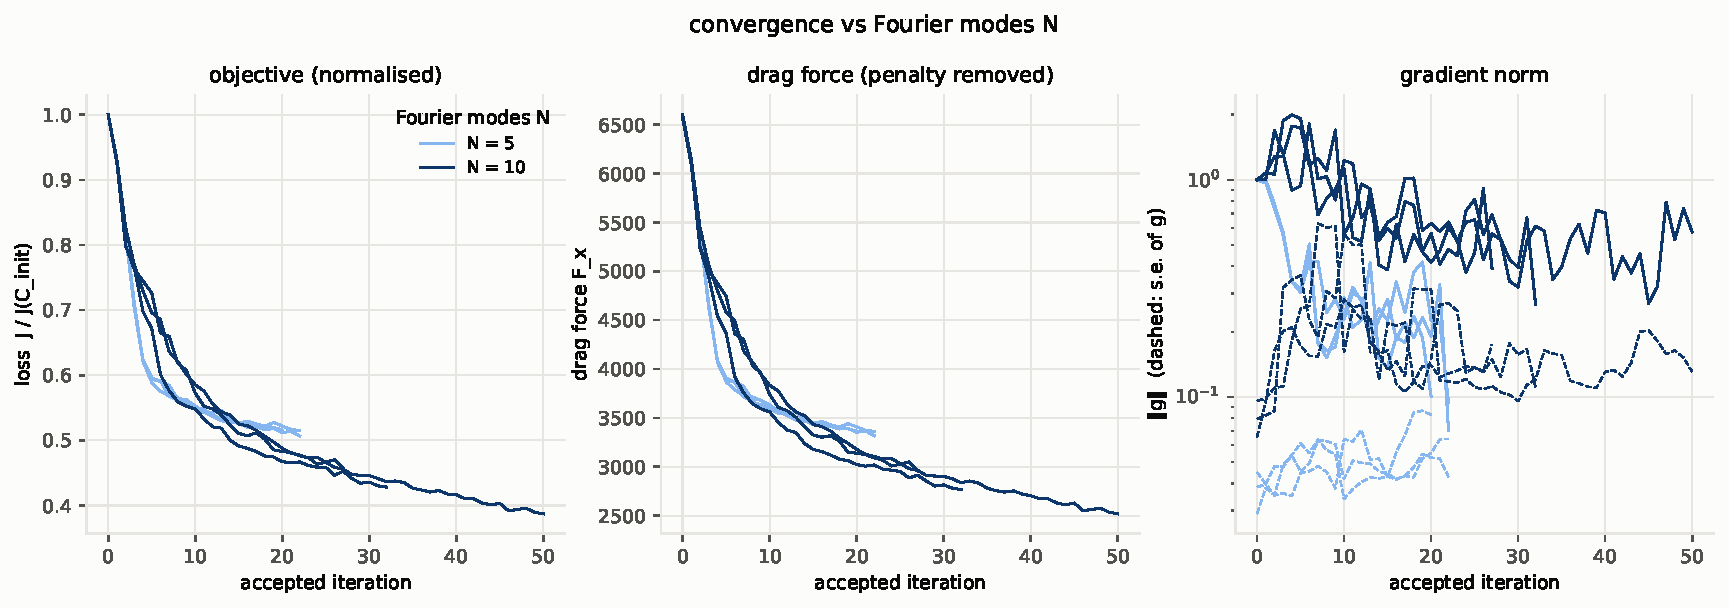
\includegraphics[width=0.92\textwidth,height=0.40\textheight,keepaspectratio]{summary/pass2_convergence_vs_nfourier.pdf}\caption{This figure shows the objective and the gradient norm against iteration. The runs differ only in N\_FOURIER. Pass 2 used the same settings with N\_ITER = 50 and SEED0 = 0, 100 and 200.}\end{figure}
\begin{figure}[H]\centering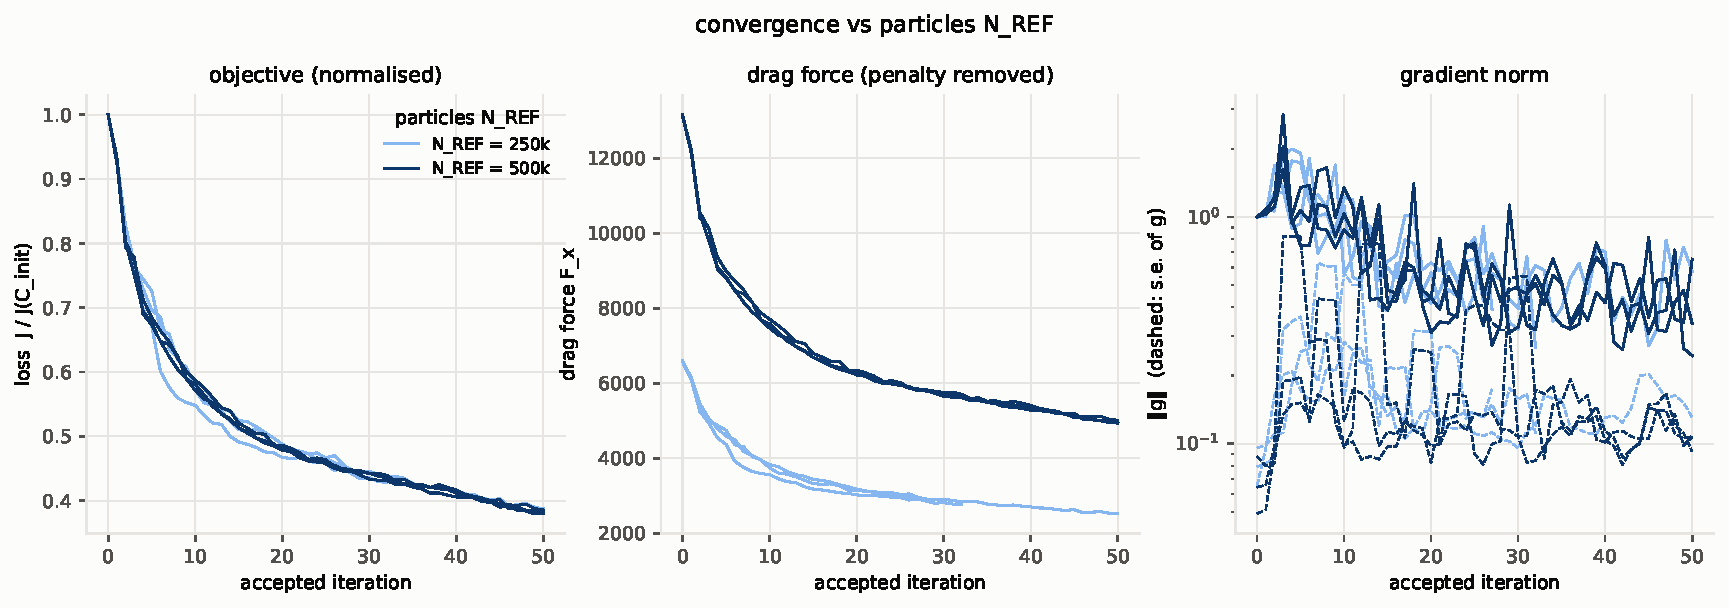
\includegraphics[width=0.92\textwidth,height=0.40\textheight,keepaspectratio]{summary/pass2_convergence_vs_nref.pdf}\caption{This figure shows the objective and the gradient norm against iteration. The runs differ only in N\_REF. Pass 2 used the same settings with N\_ITER = 50 and SEED0 = 0, 100 and 200.}\end{figure}
\begin{figure}[H]\centering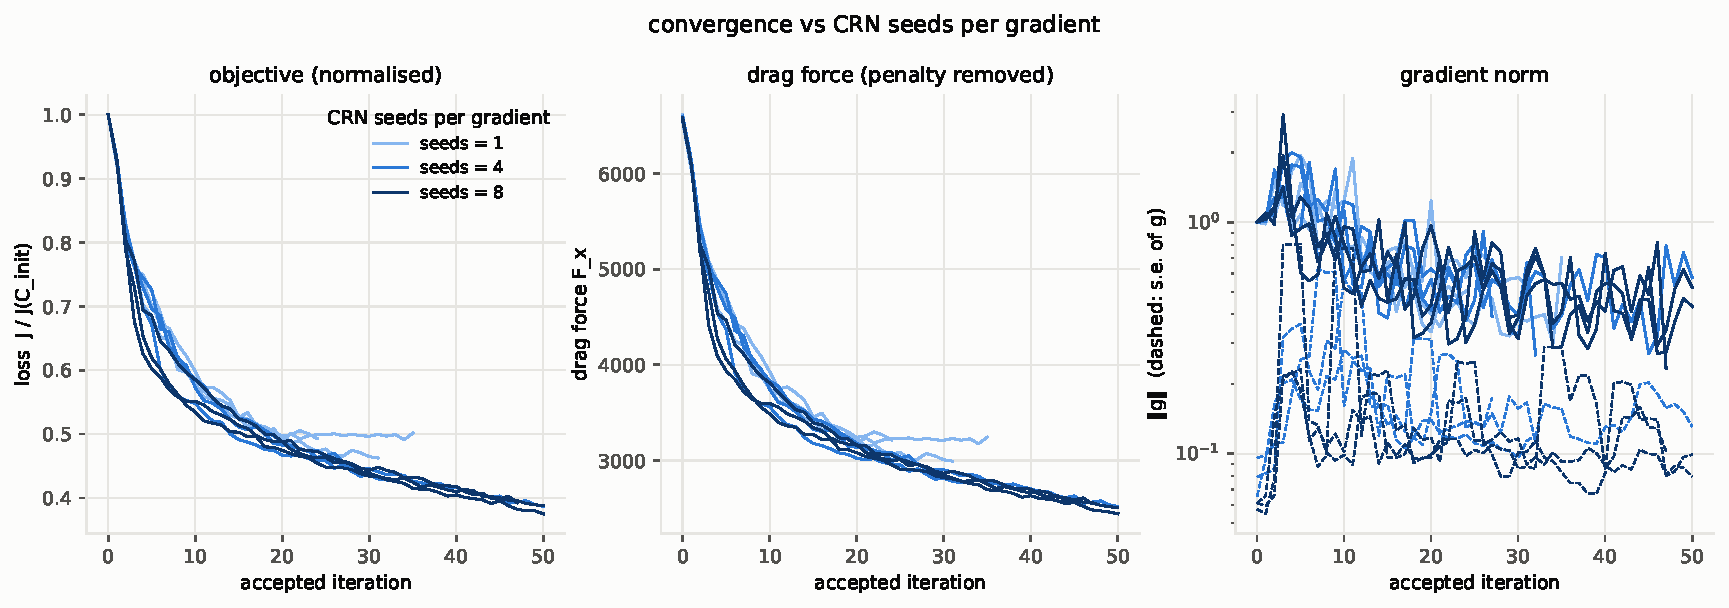
\includegraphics[width=0.92\textwidth,height=0.40\textheight,keepaspectratio]{summary/pass2_convergence_vs_seeds.pdf}\caption{This figure shows the objective and the gradient norm against iteration. The runs differ only in N\_AVG. Pass 2 used the same settings with N\_ITER = 50 and SEED0 = 0, 100 and 200.}\end{figure}
\begin{figure}[H]\centering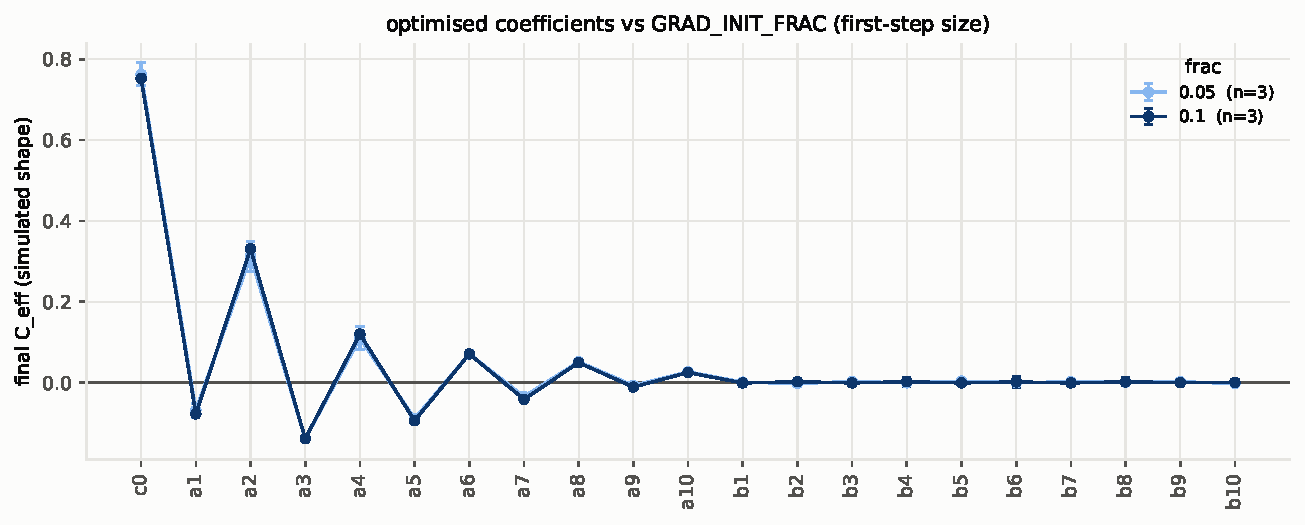
\includegraphics[width=0.92\textwidth,height=0.40\textheight,keepaspectratio]{summary/pass2_final_coeffs_vs_frac.pdf}\caption{This figure shows the final shape coefficients against GRAD\_INIT\_FRAC. Pass 2 used the same settings with N\_ITER = 50 and SEED0 = 0, 100 and 200.}\end{figure}
\begin{figure}[H]\centering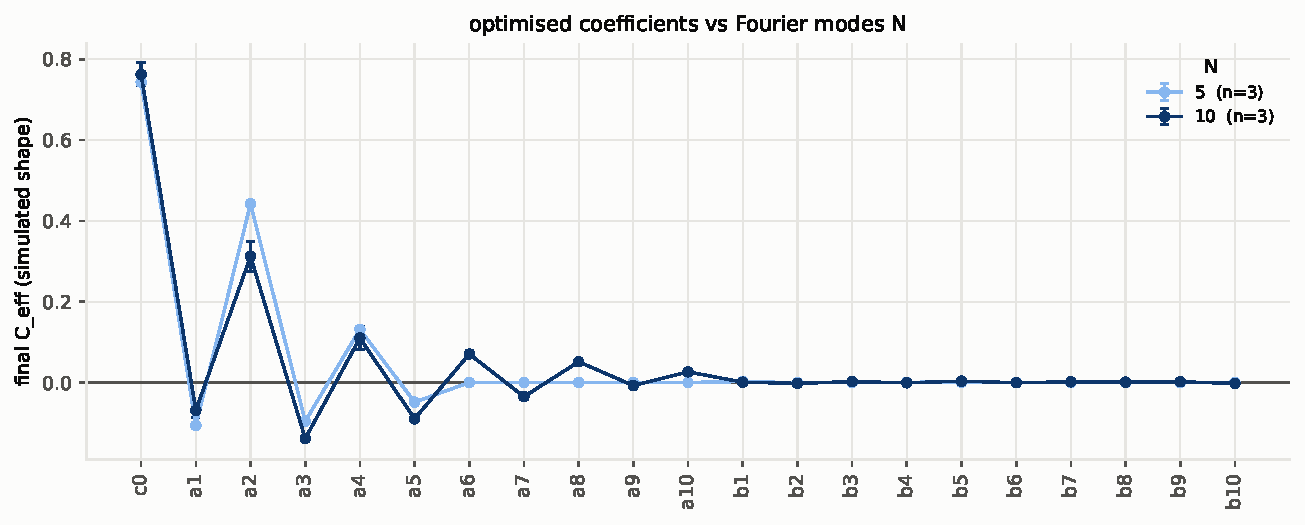
\includegraphics[width=0.92\textwidth,height=0.40\textheight,keepaspectratio]{summary/pass2_final_coeffs_vs_nfourier.pdf}\caption{This figure shows the final shape coefficients against N\_FOURIER. Pass 2 used the same settings with N\_ITER = 50 and SEED0 = 0, 100 and 200.}\end{figure}
\begin{figure}[H]\centering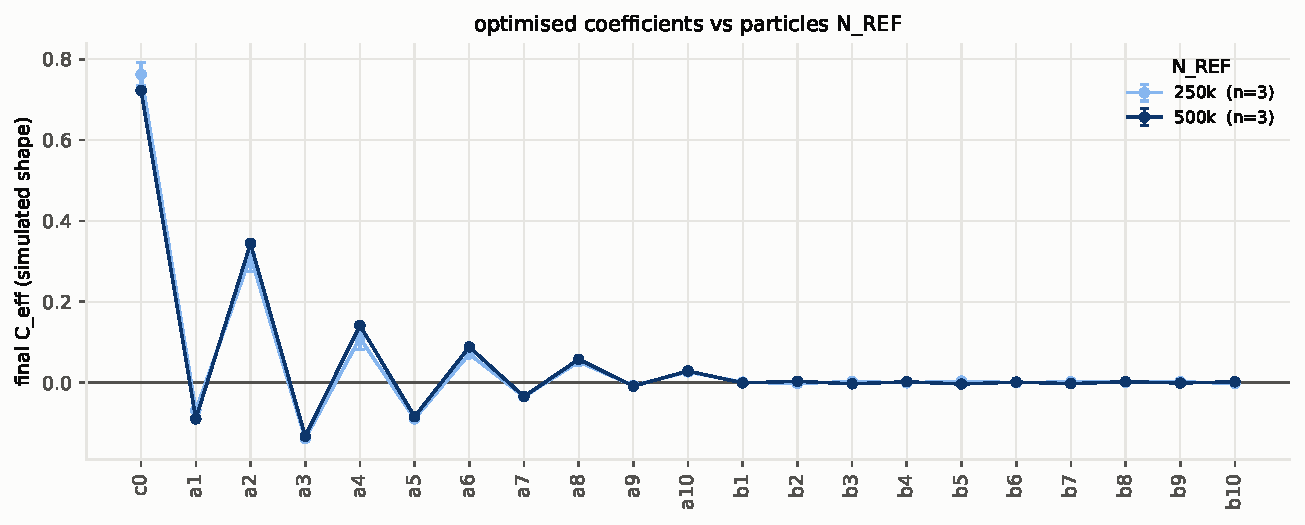
\includegraphics[width=0.92\textwidth,height=0.40\textheight,keepaspectratio]{summary/pass2_final_coeffs_vs_nref.pdf}\caption{This figure shows the final shape coefficients against N\_REF. Pass 2 used the same settings with N\_ITER = 50 and SEED0 = 0, 100 and 200.}\end{figure}
\begin{figure}[H]\centering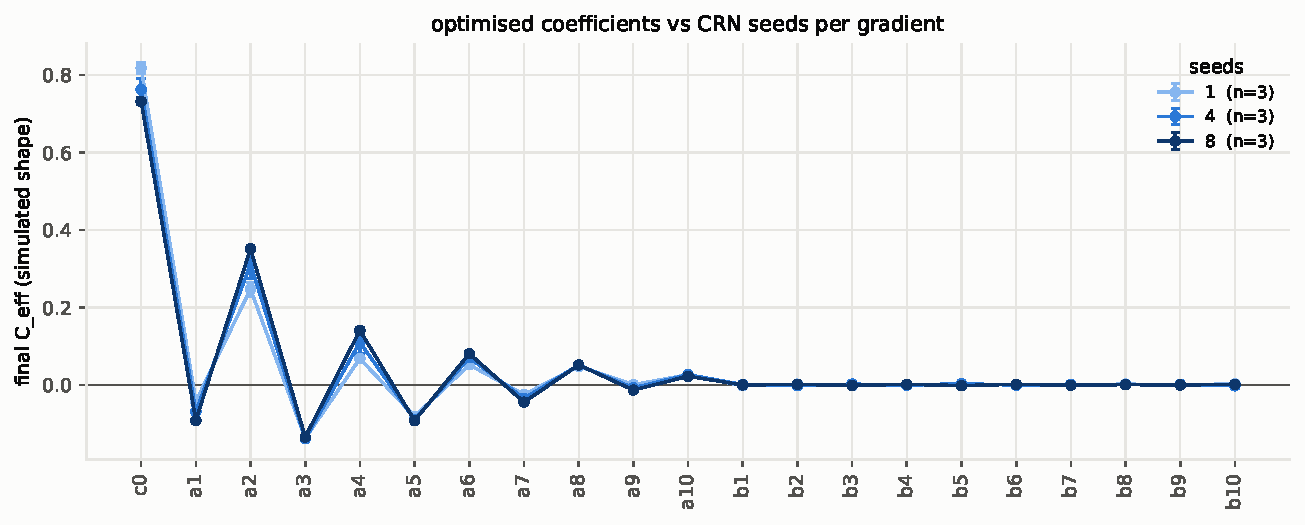
\includegraphics[width=0.92\textwidth,height=0.40\textheight,keepaspectratio]{summary/pass2_final_coeffs_vs_seeds.pdf}\caption{This figure shows the final shape coefficients against N\_AVG. Pass 2 used the same settings with N\_ITER = 50 and SEED0 = 0, 100 and 200.}\end{figure}
\begin{figure}[H]\centering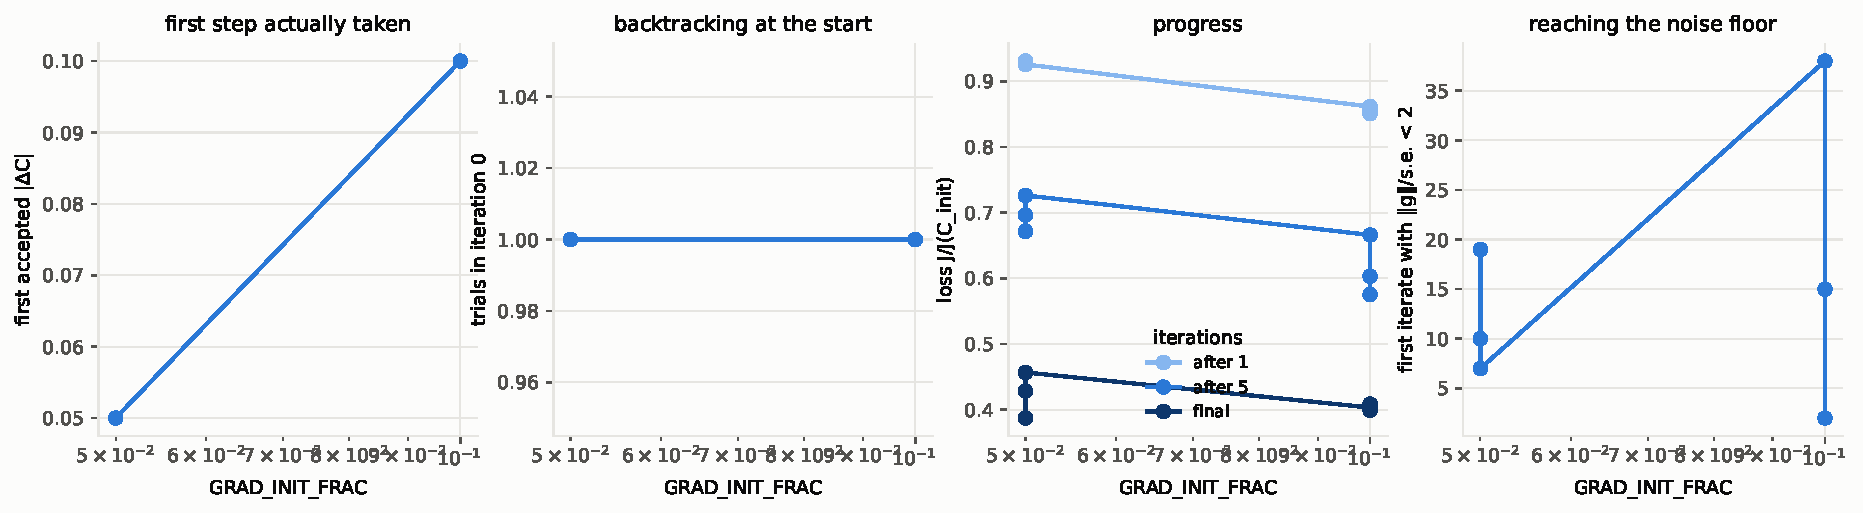
\includegraphics[width=0.92\textwidth,height=0.40\textheight,keepaspectratio]{summary/pass2_grad_init_frac_effects.pdf}\caption{This figure shows how the first-step size affects the first accepted step, the number of backtracks at iteration 0, and the objective after 1, 5 and 20 iterations. Pass 2 used the same settings with N\_ITER = 50 and SEED0 = 0, 100 and 200.}\end{figure}
\begin{figure}[H]\centering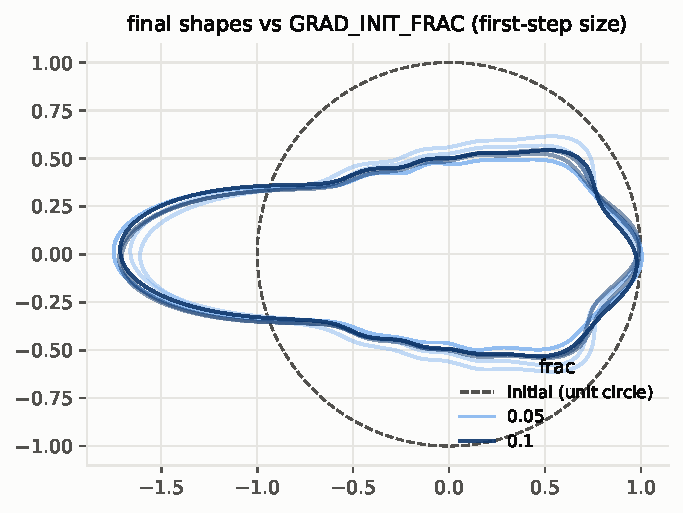
\includegraphics[width=0.92\textwidth,height=0.40\textheight,keepaspectratio]{summary/pass2_shapes_vs_frac.pdf}\caption{This figure shows the final shapes for each value of GRAD\_INIT\_FRAC. Pass 2 used the same settings with N\_ITER = 50 and SEED0 = 0, 100 and 200.}\end{figure}
\begin{figure}[H]\centering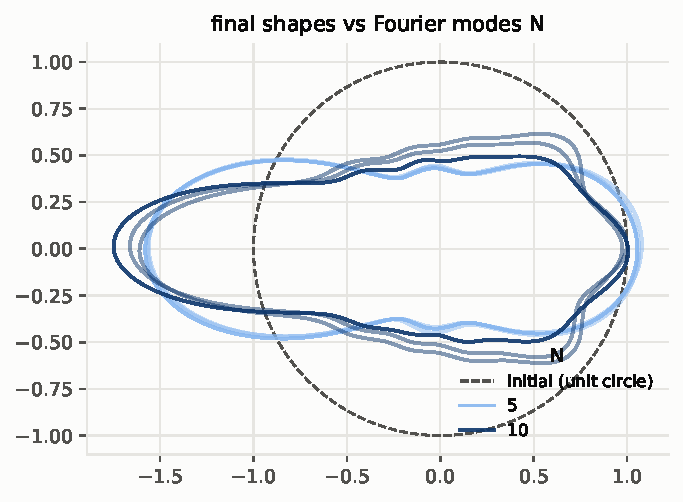
\includegraphics[width=0.92\textwidth,height=0.40\textheight,keepaspectratio]{summary/pass2_shapes_vs_nfourier.pdf}\caption{This figure shows the final shapes for each value of N\_FOURIER. Pass 2 used the same settings with N\_ITER = 50 and SEED0 = 0, 100 and 200.}\end{figure}
\begin{figure}[H]\centering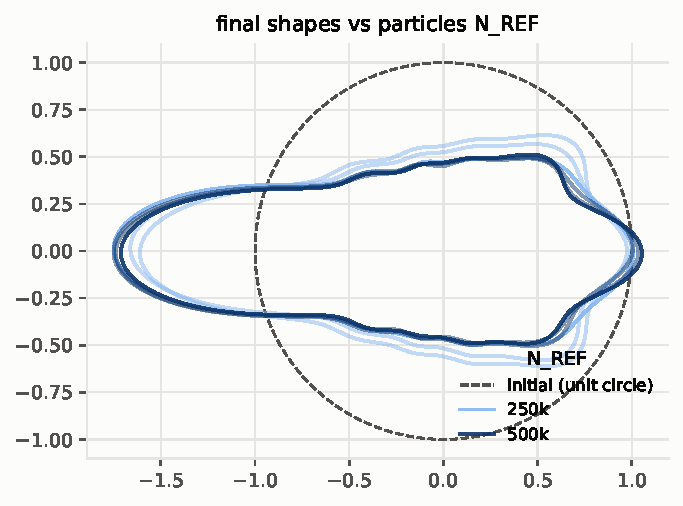
\includegraphics[width=0.92\textwidth,height=0.40\textheight,keepaspectratio]{summary/pass2_shapes_vs_nref.pdf}\caption{This figure shows the final shapes for each value of N\_REF. Pass 2 used the same settings with N\_ITER = 50 and SEED0 = 0, 100 and 200.}\end{figure}
\begin{figure}[H]\centering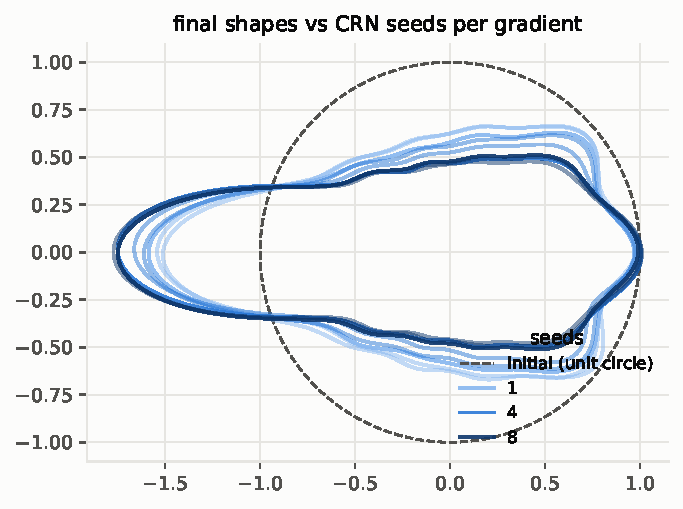
\includegraphics[width=0.92\textwidth,height=0.40\textheight,keepaspectratio]{summary/pass2_shapes_vs_seeds.pdf}\caption{This figure shows the final shapes for each value of N\_AVG. Pass 2 used the same settings with N\_ITER = 50 and SEED0 = 0, 100 and 200.}\end{figure}
\begin{figure}[H]\centering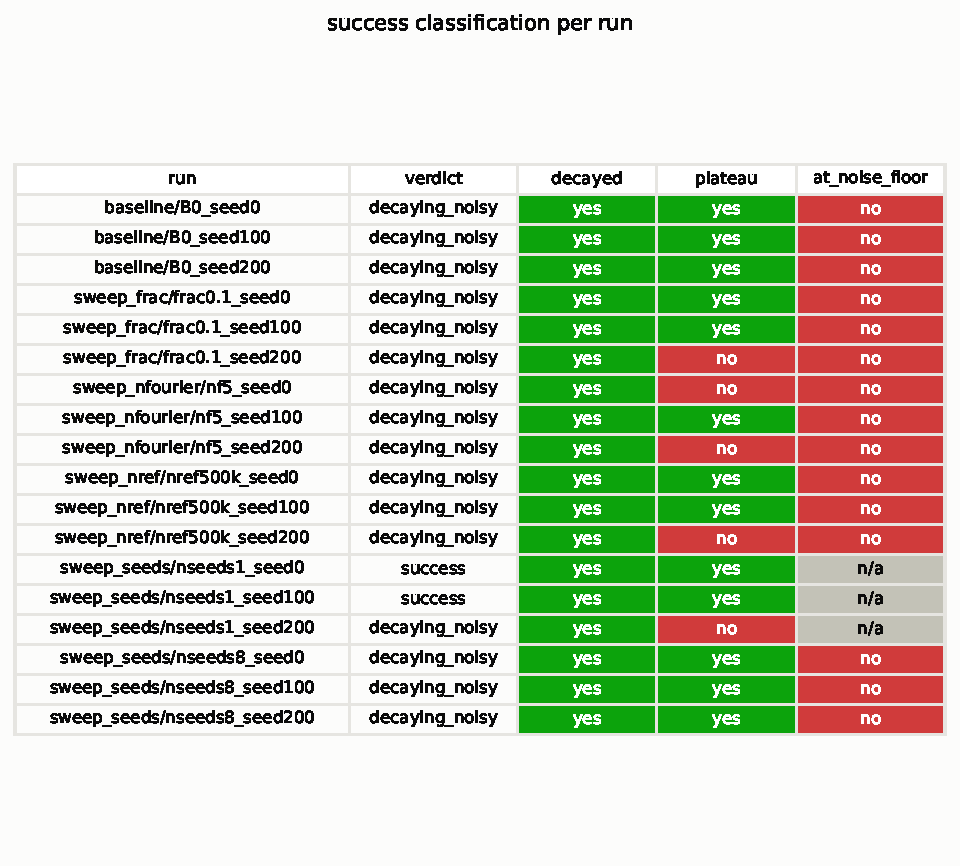
\includegraphics[width=0.92\textwidth,height=0.40\textheight,keepaspectratio]{summary/pass2_success_table.pdf}\caption{This figure shows the automatic classifier's verdict for each run. For 1-seed runs a success verdict is an artefact, because a single seed gives no noise estimate. Pass 2 used the same settings with N\_ITER = 50 and SEED0 = 0, 100 and 200.}\end{figure}
\begin{figure}[H]\centering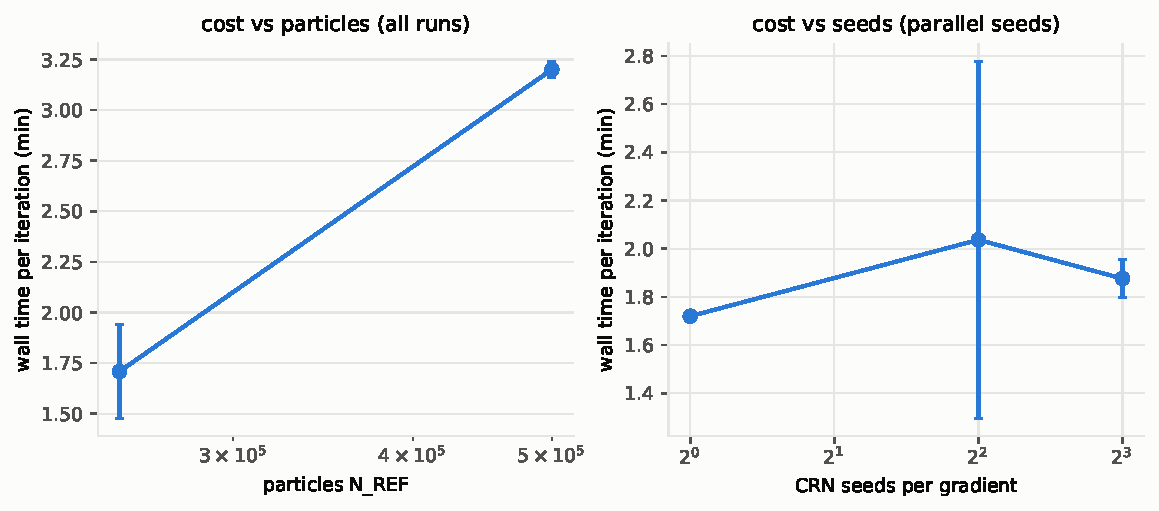
\includegraphics[width=0.92\textwidth,height=0.40\textheight,keepaspectratio]{summary/pass2_wall_per_iter.pdf}\caption{This figure shows the wall-clock time per iteration against the particle count and the number of seeds. Pass 2 used the same settings with N\_ITER = 50 and SEED0 = 0, 100 and 200.}\end{figure}
\subsection{Pass 3}
\begin{figure}[H]\centering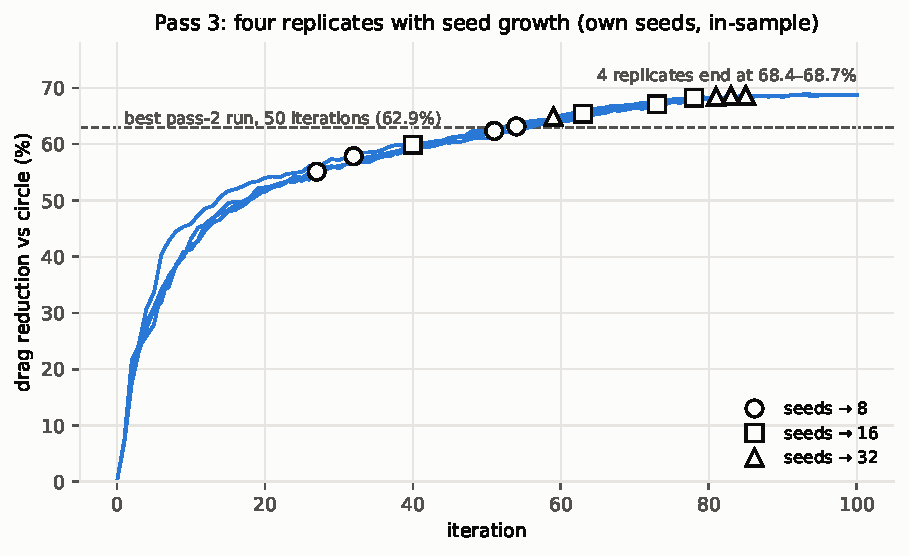
\includegraphics[width=0.92\textwidth,height=0.40\textheight,keepaspectratio]{summary/pass3_p3_growth_trajectories.pdf}\caption{This figure shows the drag reduction against iteration for the four pass-3 replicates on their own seeds. The markers show where each run doubled its seeds instead of stopping. Pass 3 used N\_REF = 250k, N\_AVG = 4, N\_AVG\_MAX = 32, N\_FOURIER = 10, GRAD\_INIT\_FRAC = 0.05, N\_ITER = 100 and SEED0 = 0, 100, 200 and 300.}\end{figure}
\begin{figure}[H]\centering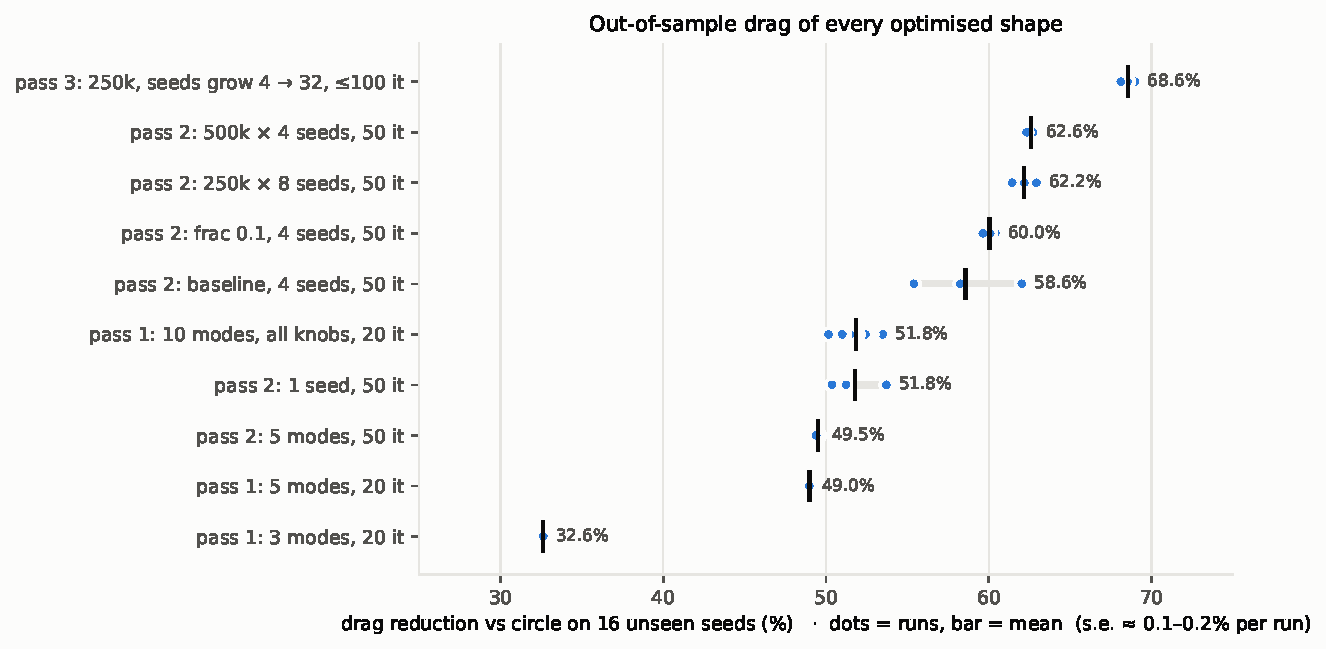
\includegraphics[width=0.92\textwidth,height=0.40\textheight,keepaspectratio]{summary/pass3_p3_heldout_by_setting.pdf}\caption{This figure shows the drag reduction of every optimised shape on 16 unseen seeds, grouped by setting. Each dot is one run, and the bar marks the mean. Pass 3 used N\_REF = 250k, N\_AVG = 4, N\_AVG\_MAX = 32, N\_FOURIER = 10, GRAD\_INIT\_FRAC = 0.05, N\_ITER = 100 and SEED0 = 0, 100, 200 and 300.}\end{figure}
\begin{figure}[H]\centering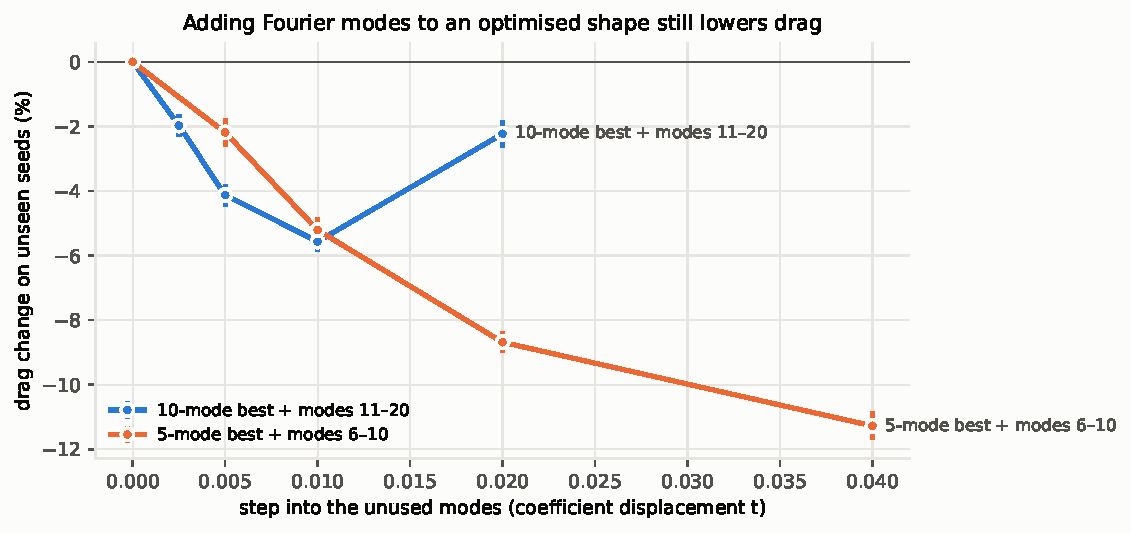
\includegraphics[width=0.92\textwidth,height=0.40\textheight,keepaspectratio]{summary/pass3_p3_mode_probes.pdf}\caption{This figure shows how the drag changes when the optimised shapes are stepped into the modes they did not use. The drag was re-measured on unseen seeds, and the error bars are $\pm 1$ standard error. Pass 3 used N\_REF = 250k, N\_AVG = 4, N\_AVG\_MAX = 32, N\_FOURIER = 10, GRAD\_INIT\_FRAC = 0.05, N\_ITER = 100 and SEED0 = 0, 100, 200 and 300.}\end{figure}
\begin{figure}[H]\centering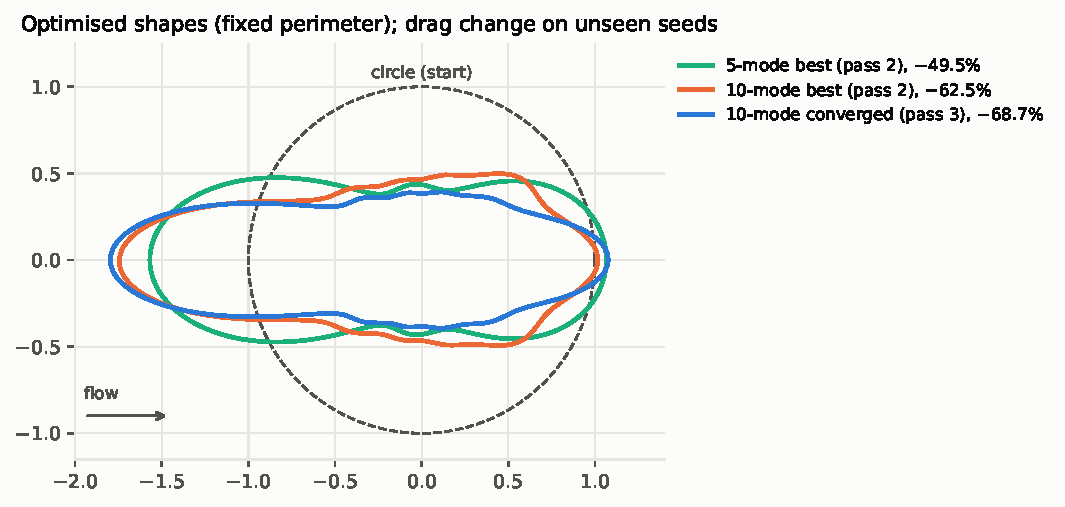
\includegraphics[width=0.92\textwidth,height=0.40\textheight,keepaspectratio]{summary/pass3_p3_shapes.pdf}\caption{This figure shows the best 5-mode and 10-mode shapes from pass 2 and the final 10-mode shape from pass 3, with their drag reductions on unseen seeds. All shapes have the same perimeter, and the gas flows from left to right. Pass 3 used N\_REF = 250k, N\_AVG = 4, N\_AVG\_MAX = 32, N\_FOURIER = 10, GRAD\_INIT\_FRAC = 0.05, N\_ITER = 100 and SEED0 = 0, 100, 200 and 300.}\end{figure}
\clearpage\section{Every run}\label{sec:perrun}This section shows each of the 38 optimisation runs. Each figure shows the drag reduction against iteration, with markers where the seed count doubled, the gradient norm with its standard error, and the final shape. The parameter values of each run are printed above its figure, and every other setting was the same in every run.
\begin{figure}[H]\centering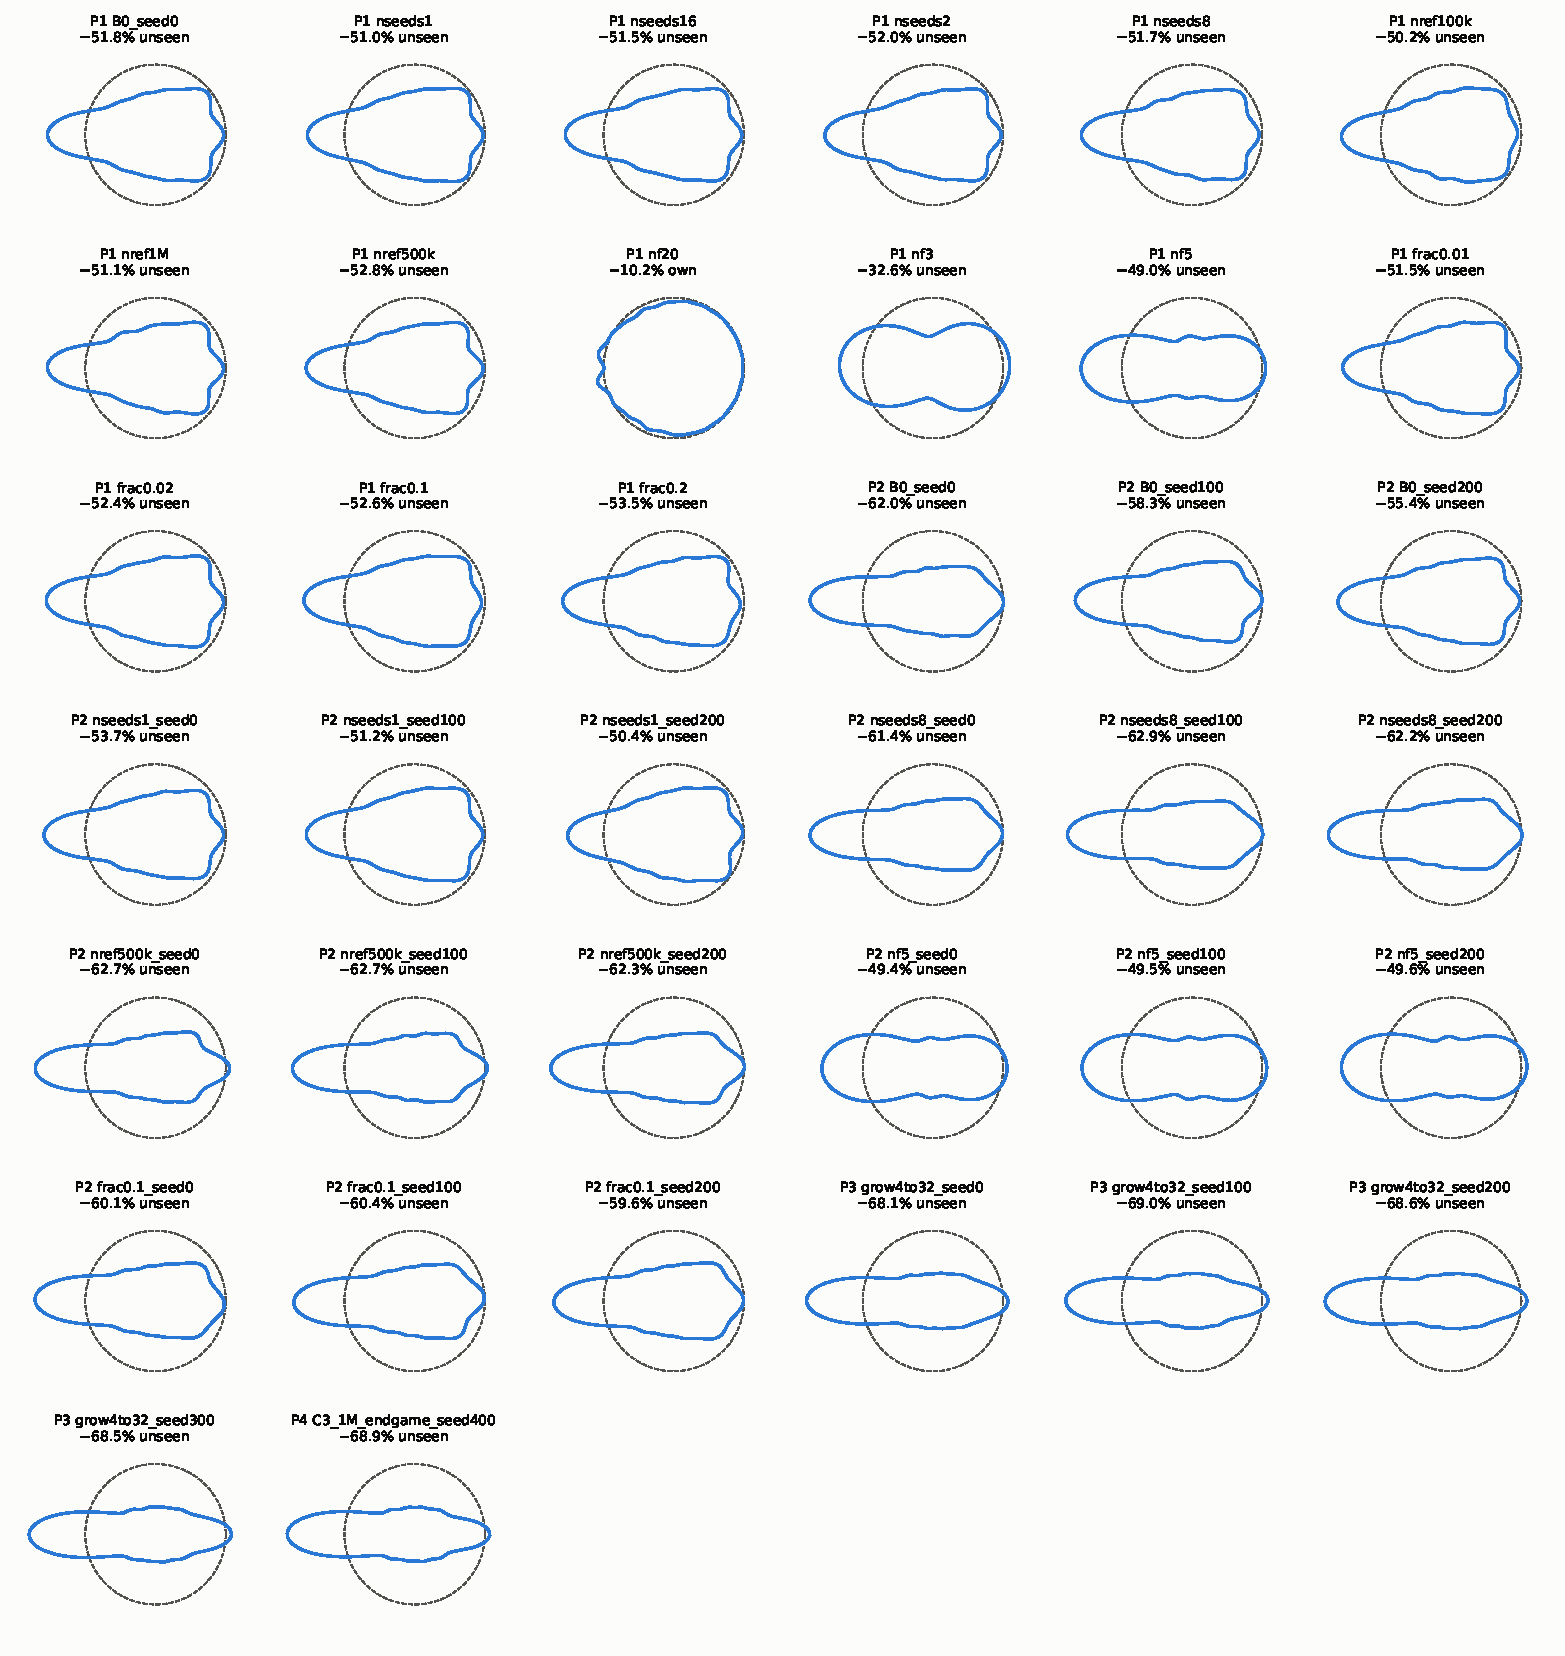
\includegraphics[width=\textwidth,height=0.85\textheight,keepaspectratio]{gallery.pdf}\caption{This figure shows every final shape, with the circle dashed. Each label gives the pass, the run and the drag reduction on unseen seeds, or on its own seeds where the shape was not re-measured.}\end{figure}
\begin{figure}[H]\centering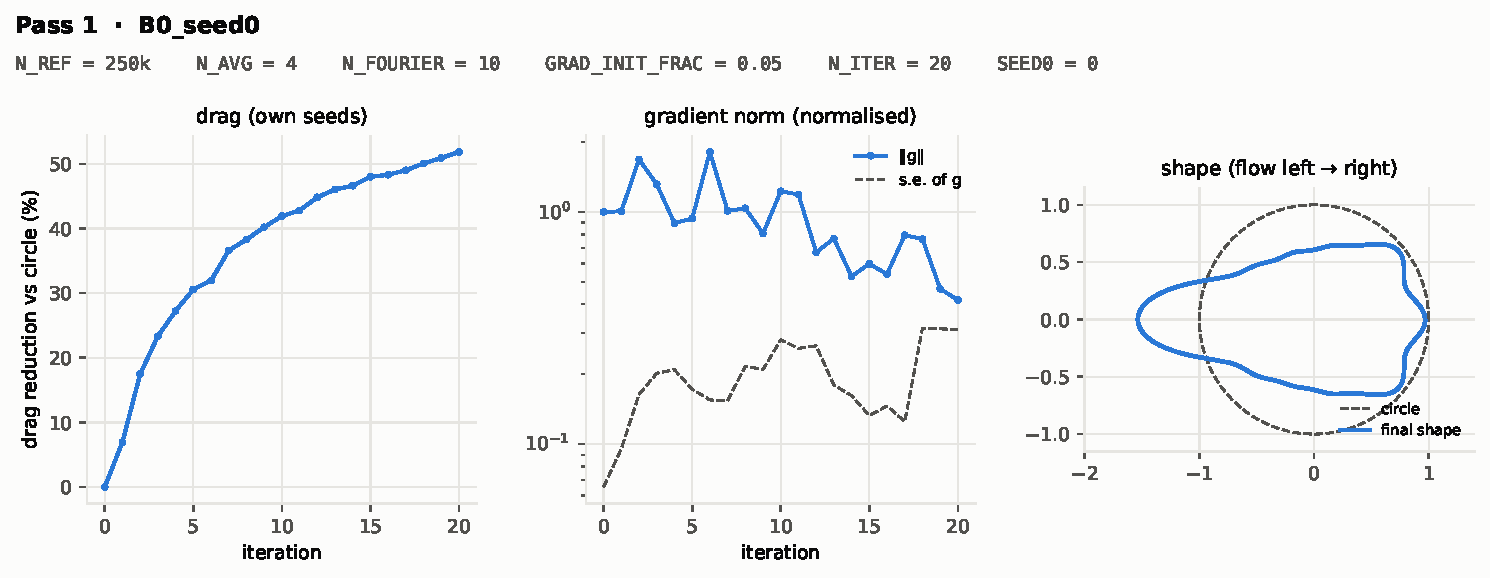
\includegraphics[width=\textwidth,height=0.42\textheight,keepaspectratio]{runs/p1_B0_seed0.pdf}\caption{Pass 1, \texttt{B0\_seed0}. The run stopped at the iteration limit after 20 iterations with 4 seeds. Its drag reduction was 51.9\% relative to the circle on its own seeds and 51.8\% relative to the circle on unseen seeds. It took 0.6 hours.}\end{figure}
\begin{figure}[H]\centering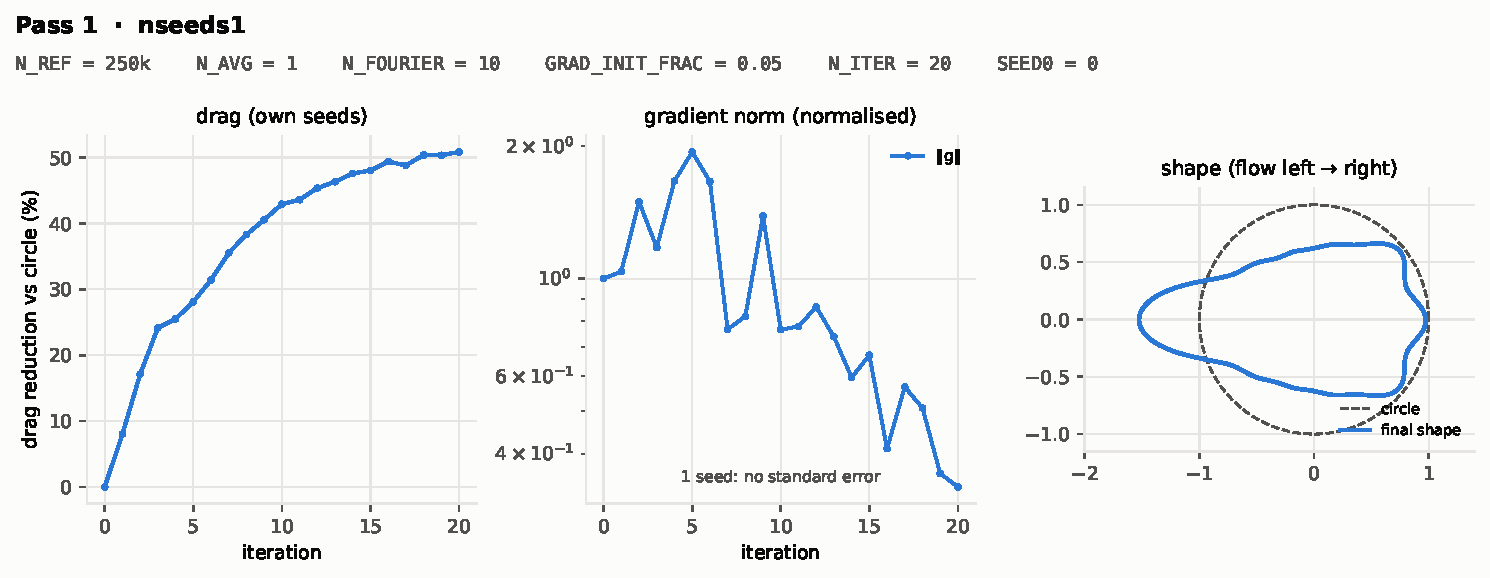
\includegraphics[width=\textwidth,height=0.42\textheight,keepaspectratio]{runs/p1_nseeds1.pdf}\caption{Pass 1, \texttt{nseeds1}. The run stopped at the iteration limit after 20 iterations with 1 seeds. Its drag reduction was 50.8\% relative to the circle on its own seeds and 51.0\% relative to the circle on unseen seeds. It took 0.5 hours.}\end{figure}
\begin{figure}[H]\centering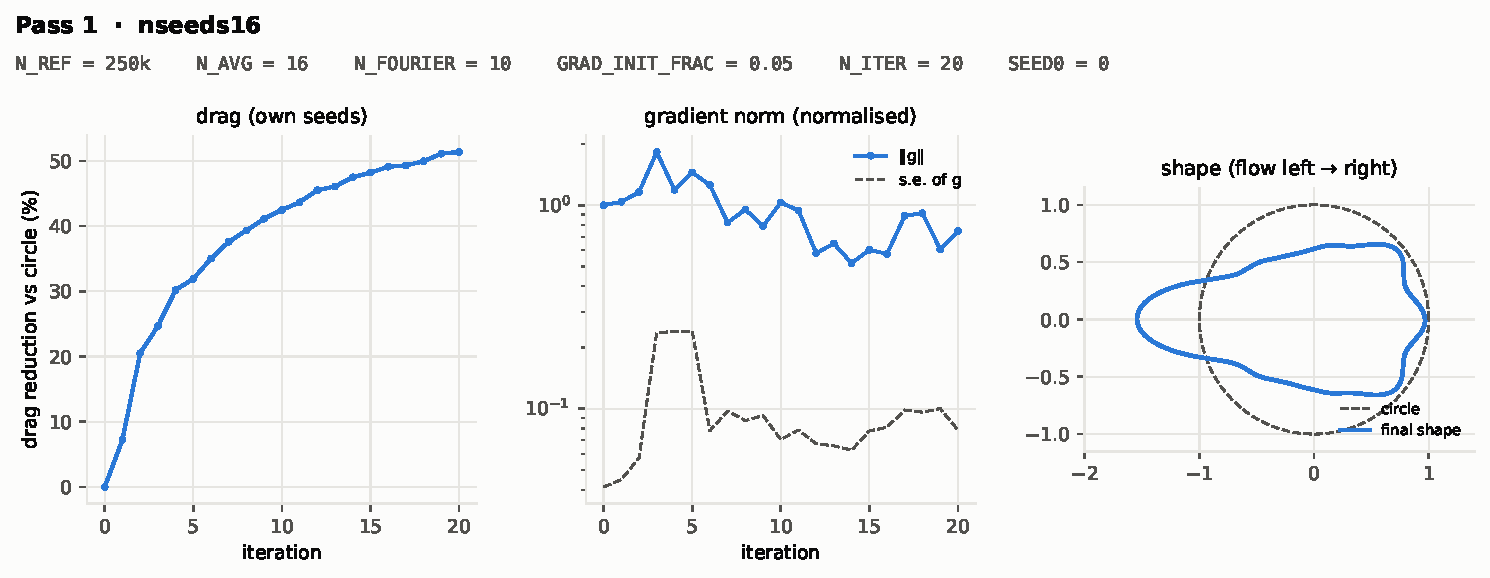
\includegraphics[width=\textwidth,height=0.42\textheight,keepaspectratio]{runs/p1_nseeds16.pdf}\caption{Pass 1, \texttt{nseeds16}. The run stopped at the iteration limit after 20 iterations with 16 seeds. Its drag reduction was 51.4\% relative to the circle on its own seeds and 51.5\% relative to the circle on unseen seeds. It took 0.8 hours.}\end{figure}
\begin{figure}[H]\centering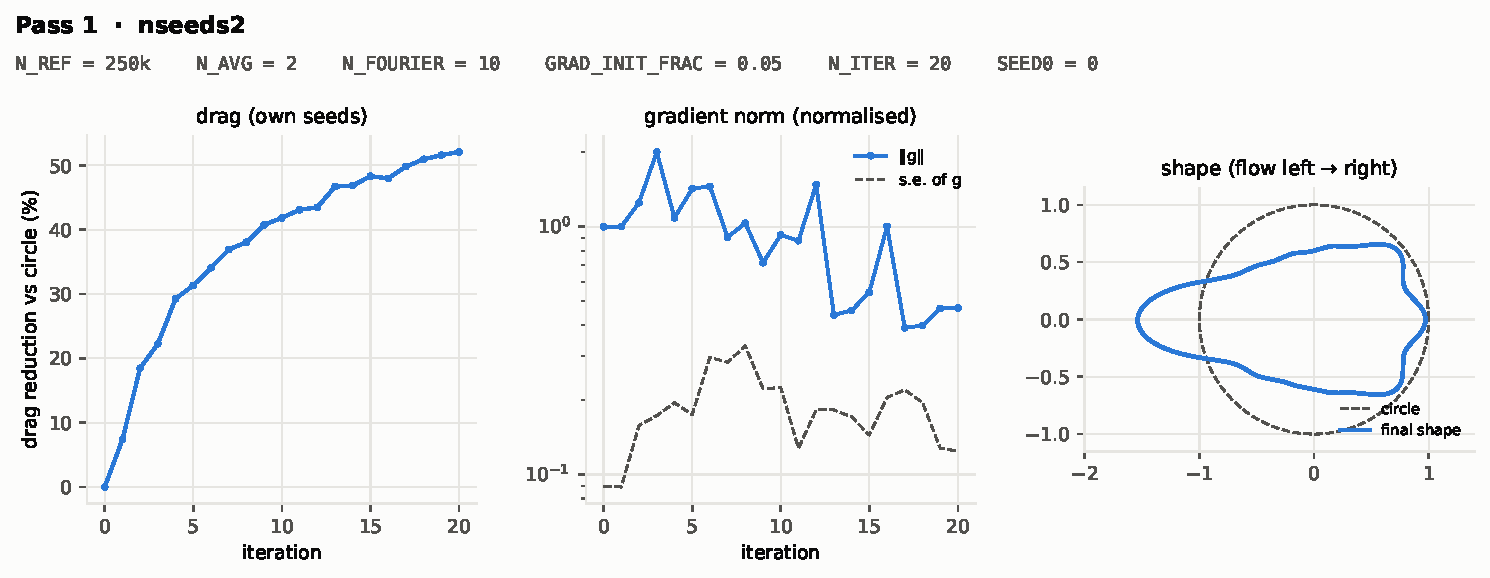
\includegraphics[width=\textwidth,height=0.42\textheight,keepaspectratio]{runs/p1_nseeds2.pdf}\caption{Pass 1, \texttt{nseeds2}. The run stopped at the iteration limit after 20 iterations with 2 seeds. Its drag reduction was 52.1\% relative to the circle on its own seeds and 52.0\% relative to the circle on unseen seeds. It took 0.6 hours.}\end{figure}
\begin{figure}[H]\centering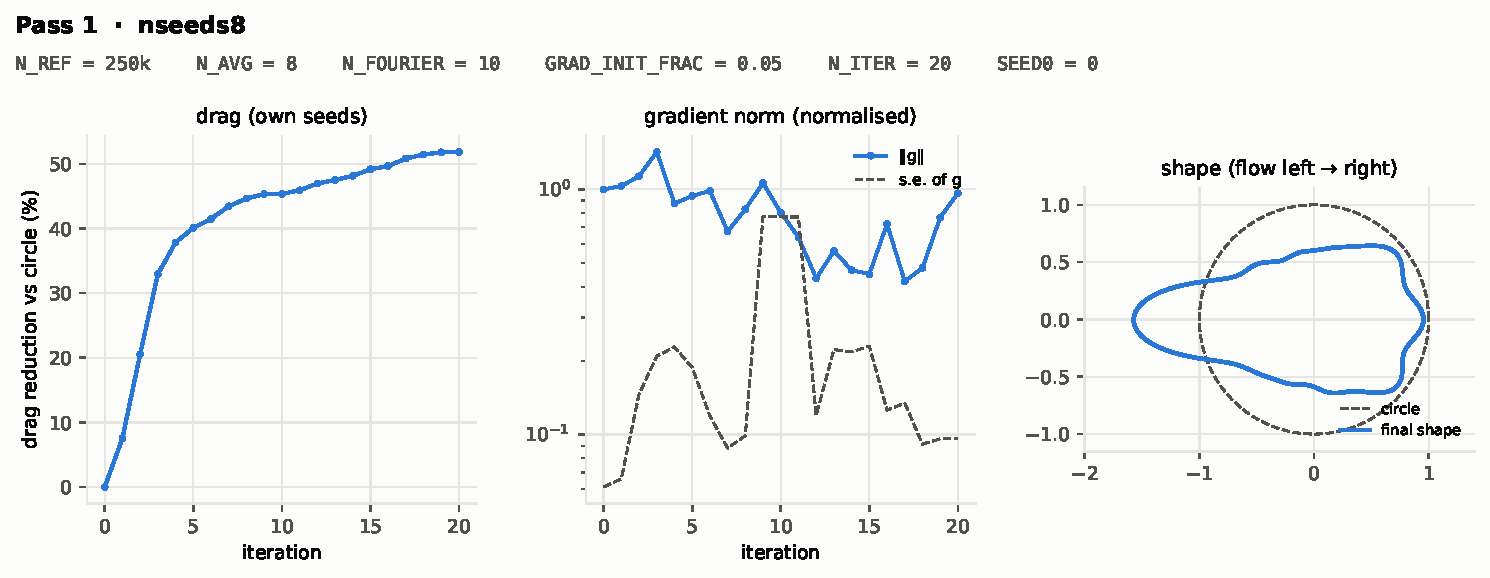
\includegraphics[width=\textwidth,height=0.42\textheight,keepaspectratio]{runs/p1_nseeds8.pdf}\caption{Pass 1, \texttt{nseeds8}. The run stopped at the iteration limit after 20 iterations with 8 seeds. Its drag reduction was 51.9\% relative to the circle on its own seeds and 51.7\% relative to the circle on unseen seeds. It took 0.6 hours.}\end{figure}
\begin{figure}[H]\centering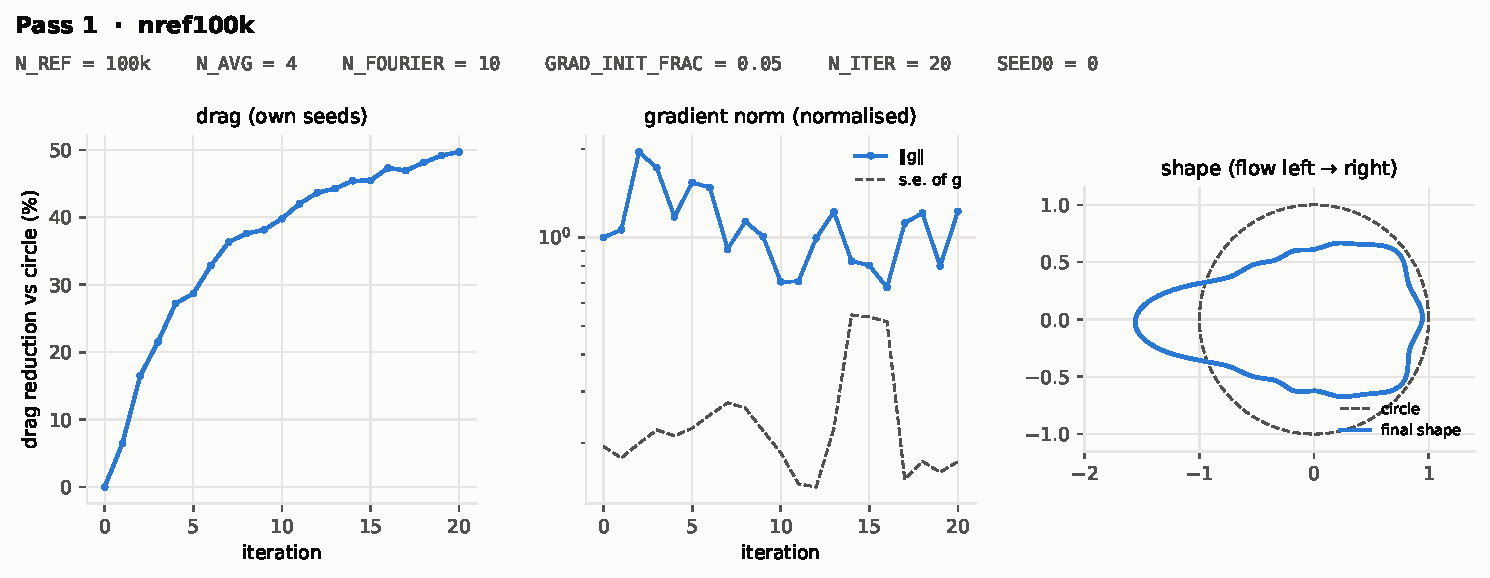
\includegraphics[width=\textwidth,height=0.42\textheight,keepaspectratio]{runs/p1_nref100k.pdf}\caption{Pass 1, \texttt{nref100k}. The run stopped at the iteration limit after 20 iterations with 4 seeds. Its drag reduction was 49.7\% relative to the circle on its own seeds and 50.2\% relative to the circle on unseen seeds. It took 0.2 hours.}\end{figure}
\begin{figure}[H]\centering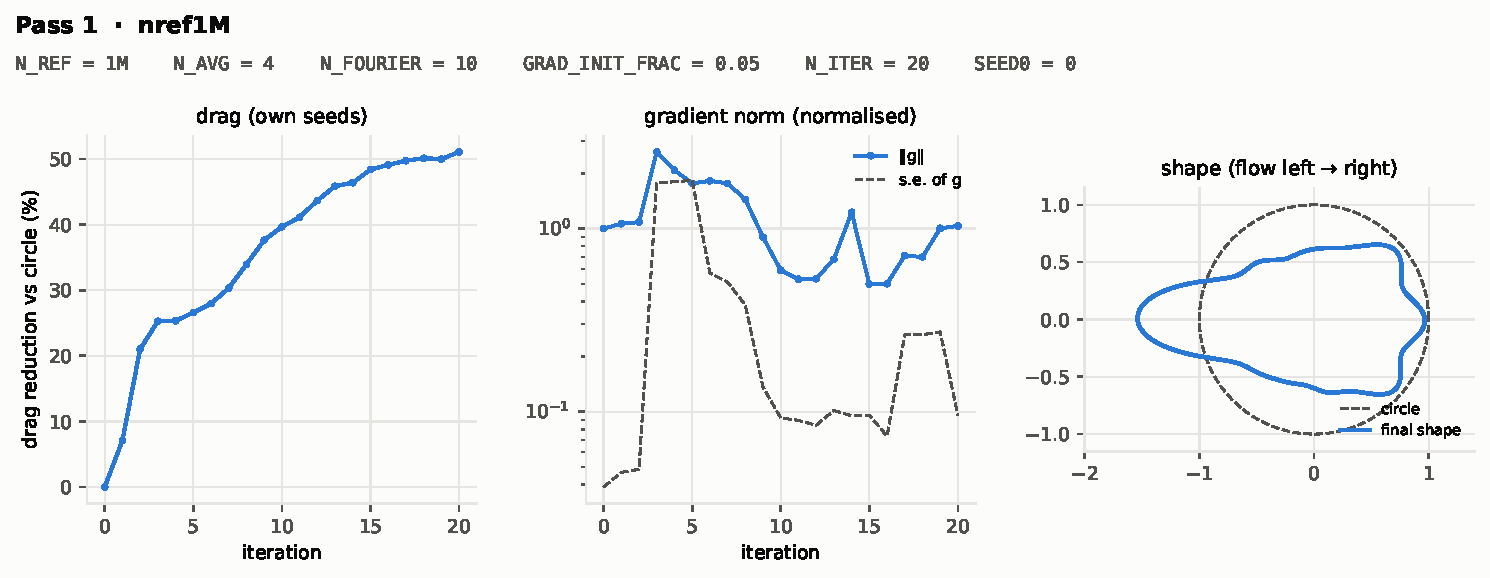
\includegraphics[width=\textwidth,height=0.42\textheight,keepaspectratio]{runs/p1_nref1M.pdf}\caption{Pass 1, \texttt{nref1M}. The run stopped at the iteration limit after 20 iterations with 4 seeds. Its drag reduction was 51.1\% relative to the circle on its own seeds and 51.1\% relative to the circle on unseen seeds. It took 1.8 hours.}\end{figure}
\begin{figure}[H]\centering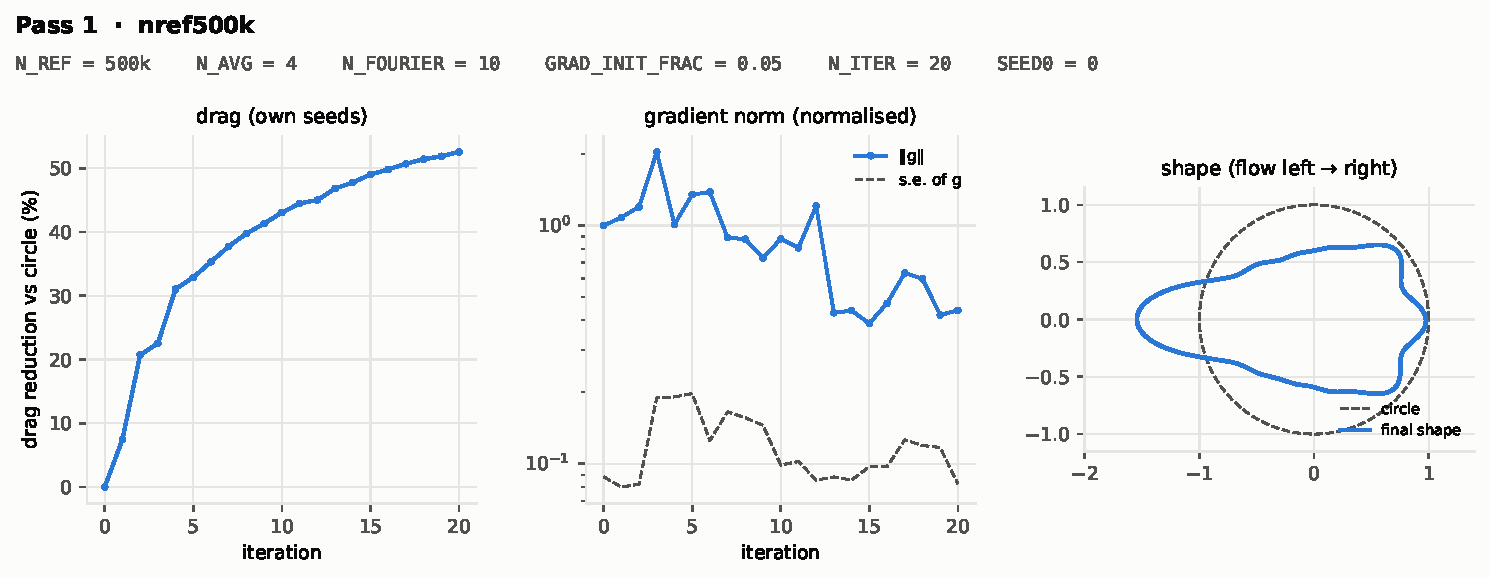
\includegraphics[width=\textwidth,height=0.42\textheight,keepaspectratio]{runs/p1_nref500k.pdf}\caption{Pass 1, \texttt{nref500k}. The run stopped at the iteration limit after 20 iterations with 4 seeds. Its drag reduction was 52.6\% relative to the circle on its own seeds and 52.8\% relative to the circle on unseen seeds. It took 0.9 hours.}\end{figure}
\begin{figure}[H]\centering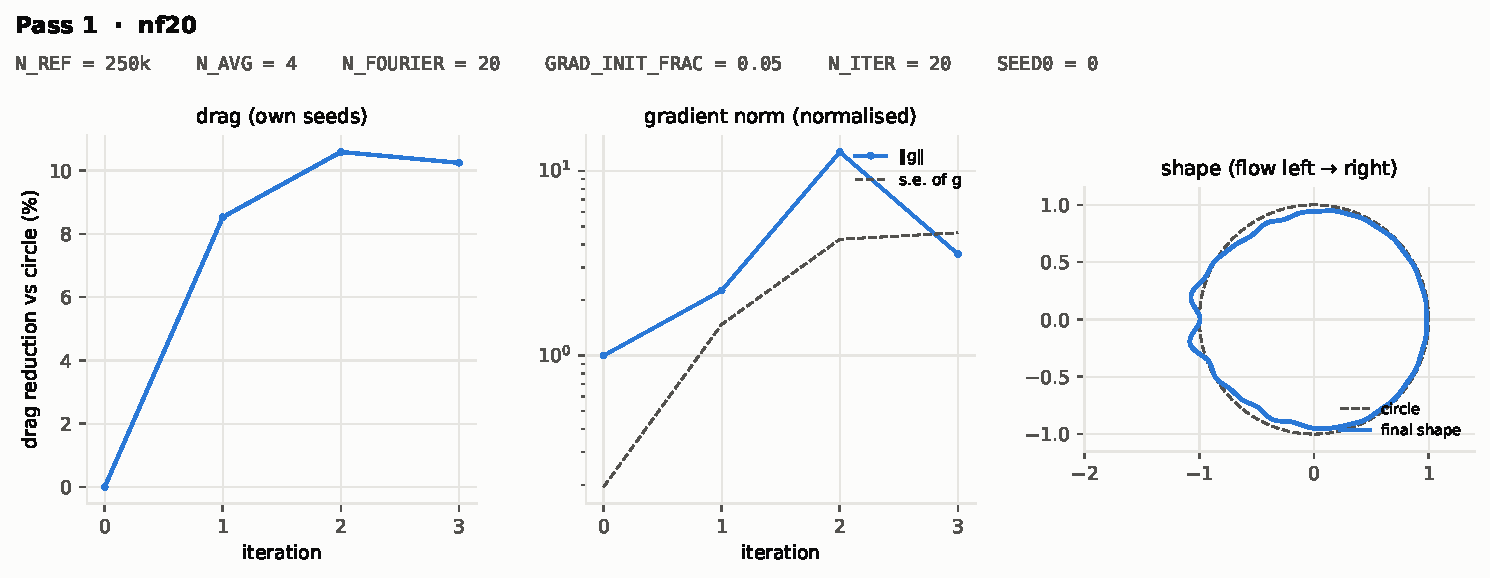
\includegraphics[width=\textwidth,height=0.42\textheight,keepaspectratio]{runs/p1_nf20.pdf}\caption{Pass 1, \texttt{nf20}. The run stopped at the noise limit after 3 iterations with 4 seeds. Its drag reduction was 10.2\% relative to the circle on its own seeds. It took 0.2 hours.}\end{figure}
\begin{figure}[H]\centering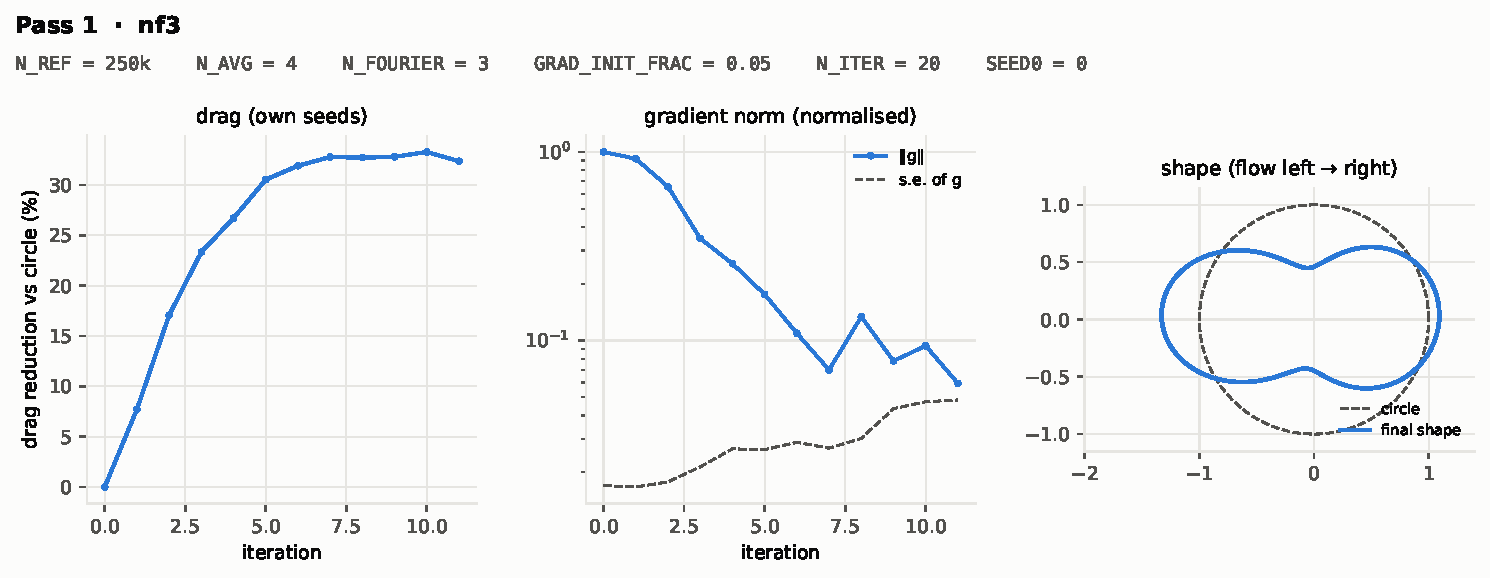
\includegraphics[width=\textwidth,height=0.42\textheight,keepaspectratio]{runs/p1_nf3.pdf}\caption{Pass 1, \texttt{nf3}. The run stopped at the noise limit after 11 iterations with 4 seeds. Its drag reduction was 32.4\% relative to the circle on its own seeds and 32.6\% relative to the circle on unseen seeds. It took 0.3 hours.}\end{figure}
\begin{figure}[H]\centering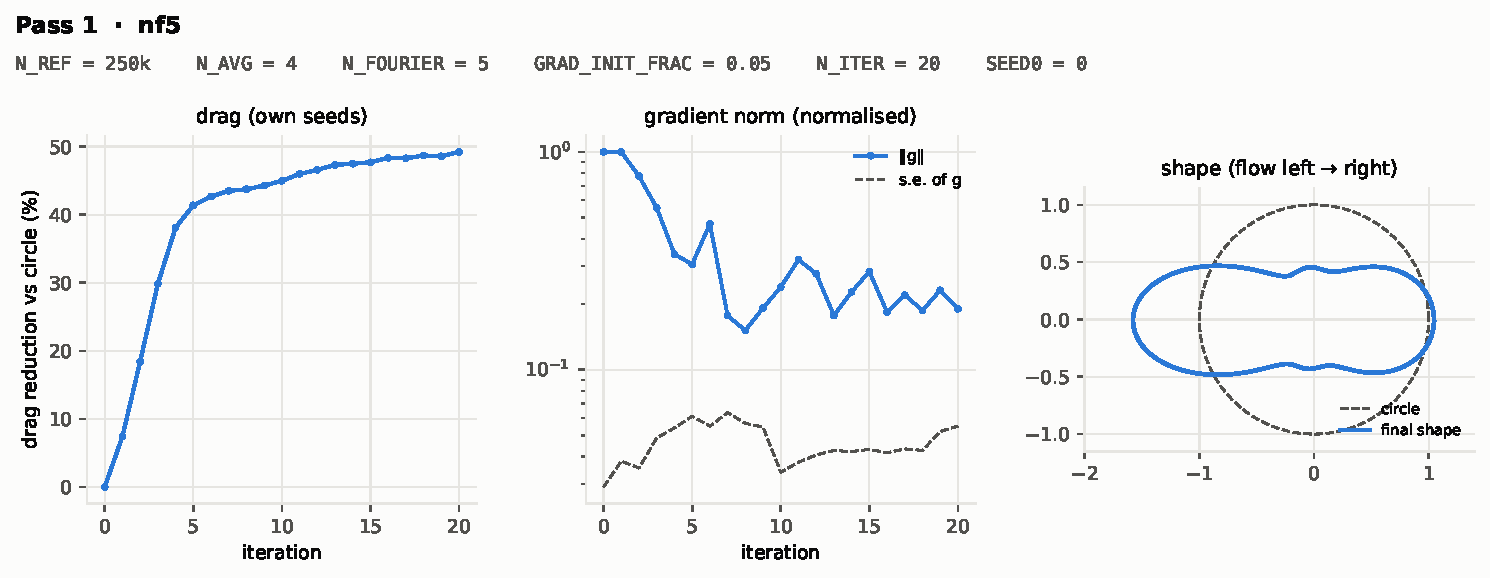
\includegraphics[width=\textwidth,height=0.42\textheight,keepaspectratio]{runs/p1_nf5.pdf}\caption{Pass 1, \texttt{nf5}. The run stopped at the iteration limit after 20 iterations with 4 seeds. Its drag reduction was 49.2\% relative to the circle on its own seeds and 49.0\% relative to the circle on unseen seeds. It took 0.4 hours.}\end{figure}
\begin{figure}[H]\centering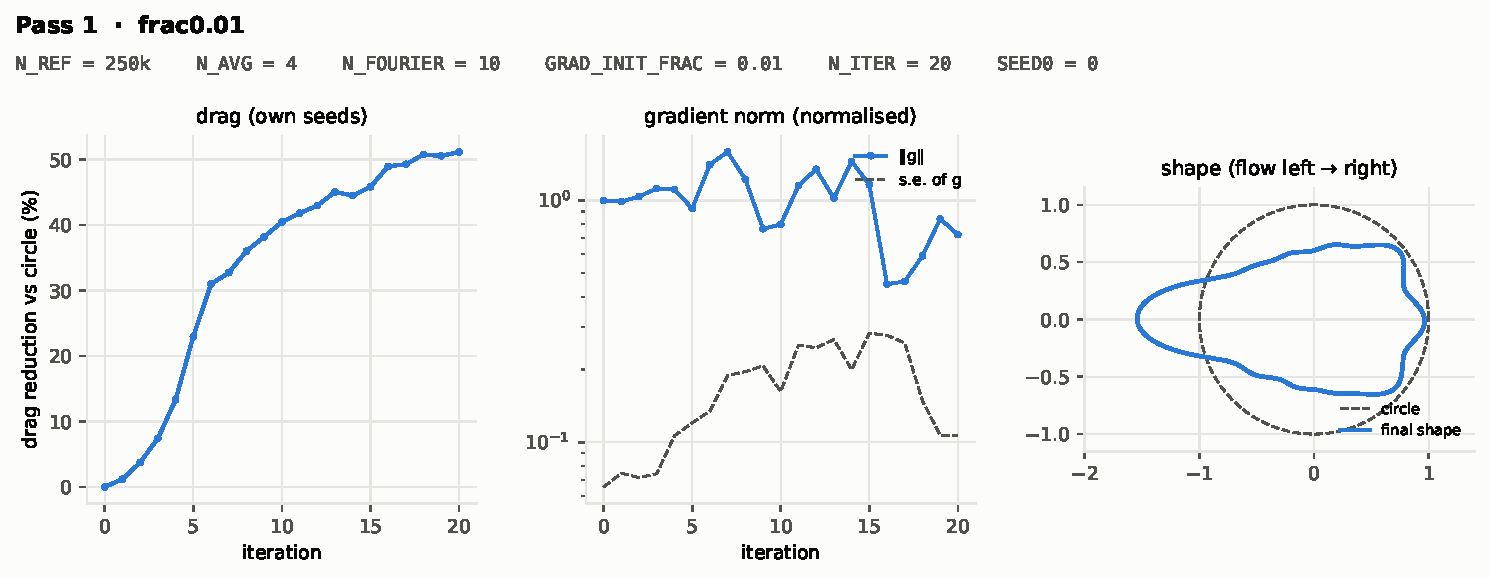
\includegraphics[width=\textwidth,height=0.42\textheight,keepaspectratio]{runs/p1_frac0.01.pdf}\caption{Pass 1, \texttt{frac0.01}. The run stopped at the iteration limit after 20 iterations with 4 seeds. Its drag reduction was 51.2\% relative to the circle on its own seeds and 51.5\% relative to the circle on unseen seeds. It took 0.6 hours.}\end{figure}
\begin{figure}[H]\centering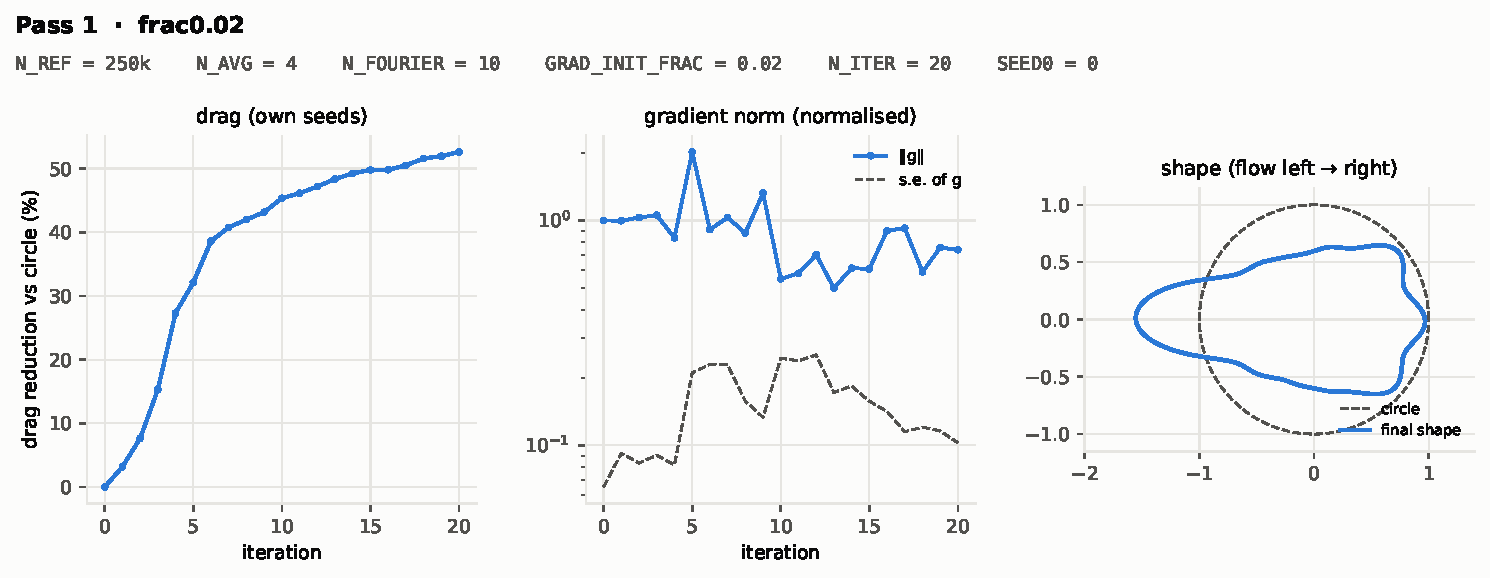
\includegraphics[width=\textwidth,height=0.42\textheight,keepaspectratio]{runs/p1_frac0.02.pdf}\caption{Pass 1, \texttt{frac0.02}. The run stopped at the iteration limit after 20 iterations with 4 seeds. Its drag reduction was 52.6\% relative to the circle on its own seeds and 52.4\% relative to the circle on unseen seeds. It took 0.6 hours.}\end{figure}
\begin{figure}[H]\centering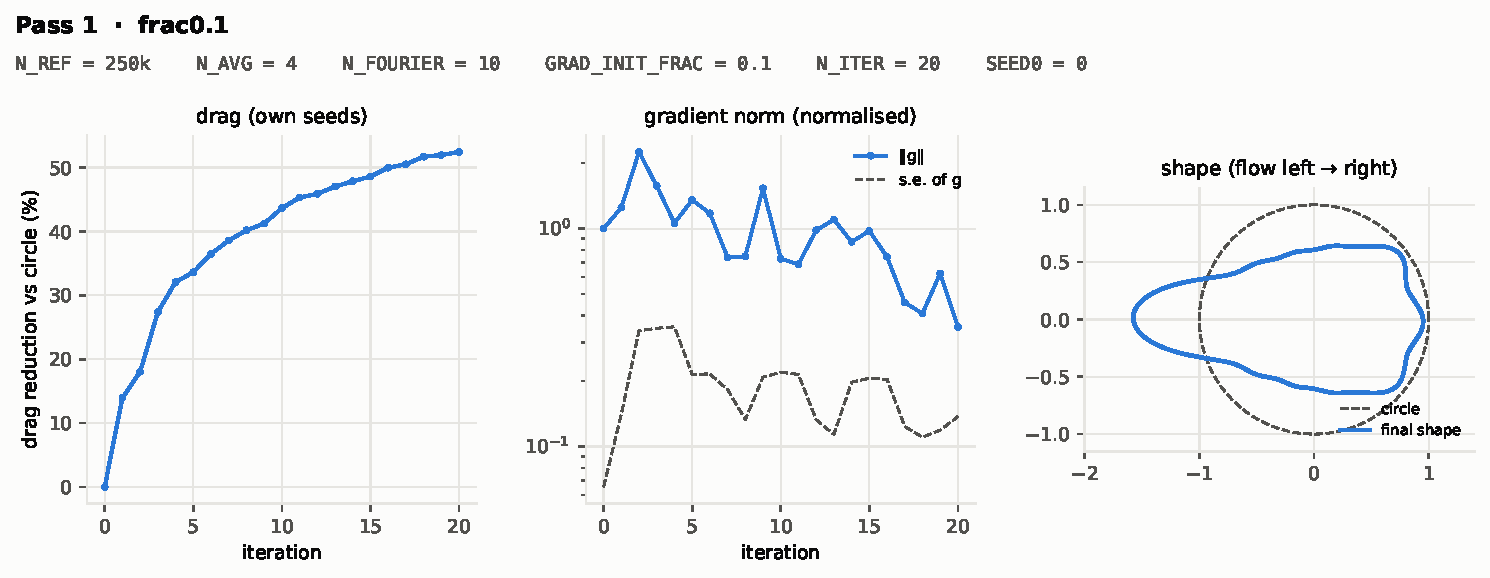
\includegraphics[width=\textwidth,height=0.42\textheight,keepaspectratio]{runs/p1_frac0.1.pdf}\caption{Pass 1, \texttt{frac0.1}. The run stopped at the iteration limit after 20 iterations with 4 seeds. Its drag reduction was 52.4\% relative to the circle on its own seeds and 52.6\% relative to the circle on unseen seeds. It took 0.7 hours.}\end{figure}
\begin{figure}[H]\centering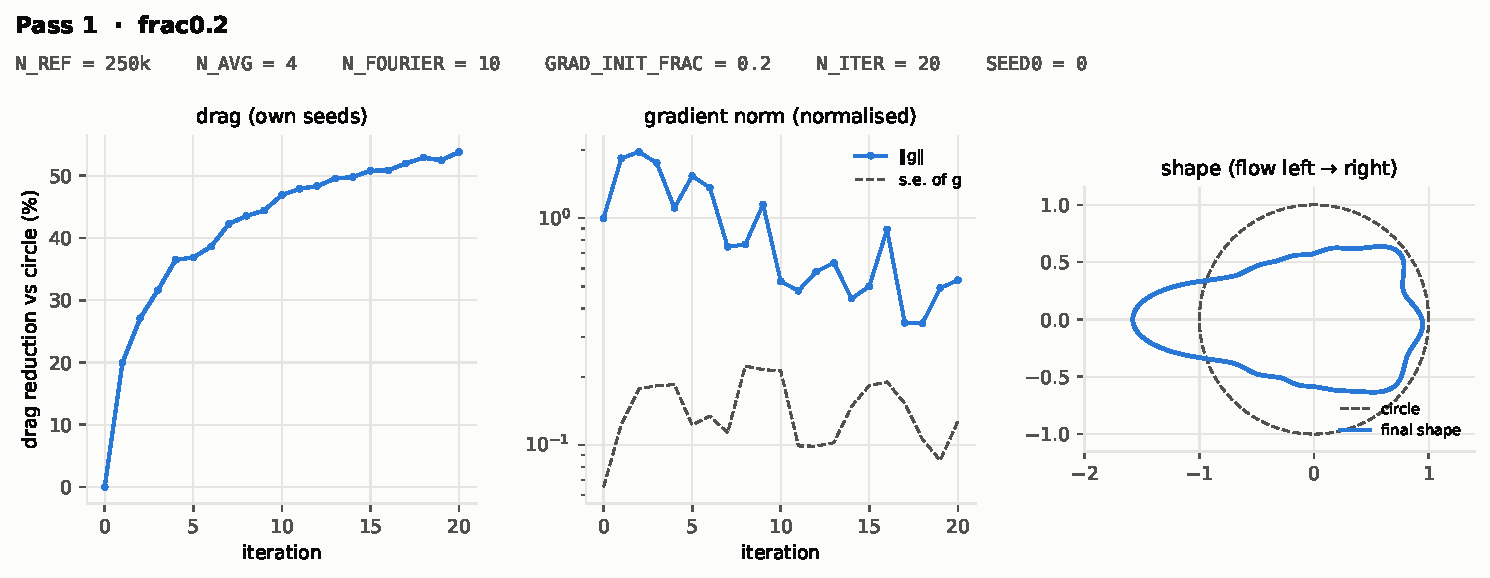
\includegraphics[width=\textwidth,height=0.42\textheight,keepaspectratio]{runs/p1_frac0.2.pdf}\caption{Pass 1, \texttt{frac0.2}. The run stopped at the iteration limit after 20 iterations with 4 seeds. Its drag reduction was 53.8\% relative to the circle on its own seeds and 53.5\% relative to the circle on unseen seeds. It took 0.6 hours.}\end{figure}
\begin{figure}[H]\centering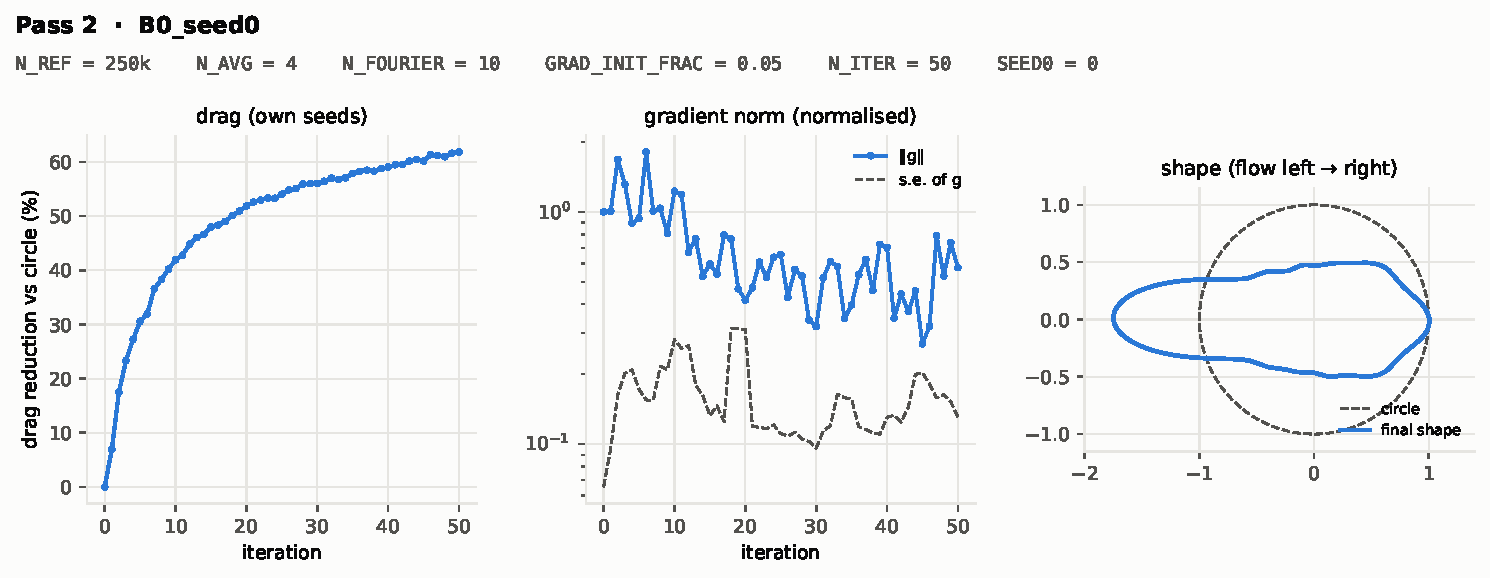
\includegraphics[width=\textwidth,height=0.42\textheight,keepaspectratio]{runs/p2_B0_seed0.pdf}\caption{Pass 2, \texttt{B0\_seed0}. The run stopped at the iteration limit after 50 iterations with 4 seeds. Its drag reduction was 61.8\% relative to the circle on its own seeds and 62.0\% relative to the circle on unseen seeds. It took 1.6 hours.}\end{figure}
\begin{figure}[H]\centering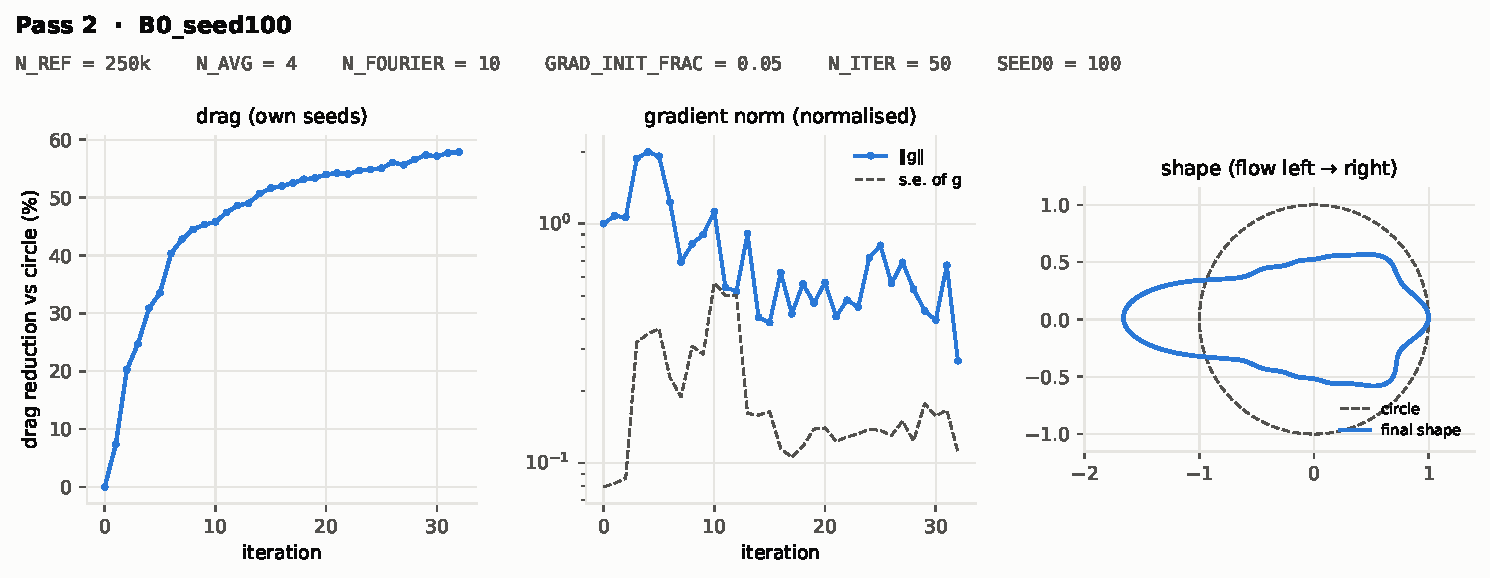
\includegraphics[width=\textwidth,height=0.42\textheight,keepaspectratio]{runs/p2_B0_seed100.pdf}\caption{Pass 2, \texttt{B0\_seed100}. The run stopped at the noise limit after 32 iterations with 4 seeds. Its drag reduction was 57.9\% relative to the circle on its own seeds and 58.3\% relative to the circle on unseen seeds. It took 1.1 hours.}\end{figure}
\begin{figure}[H]\centering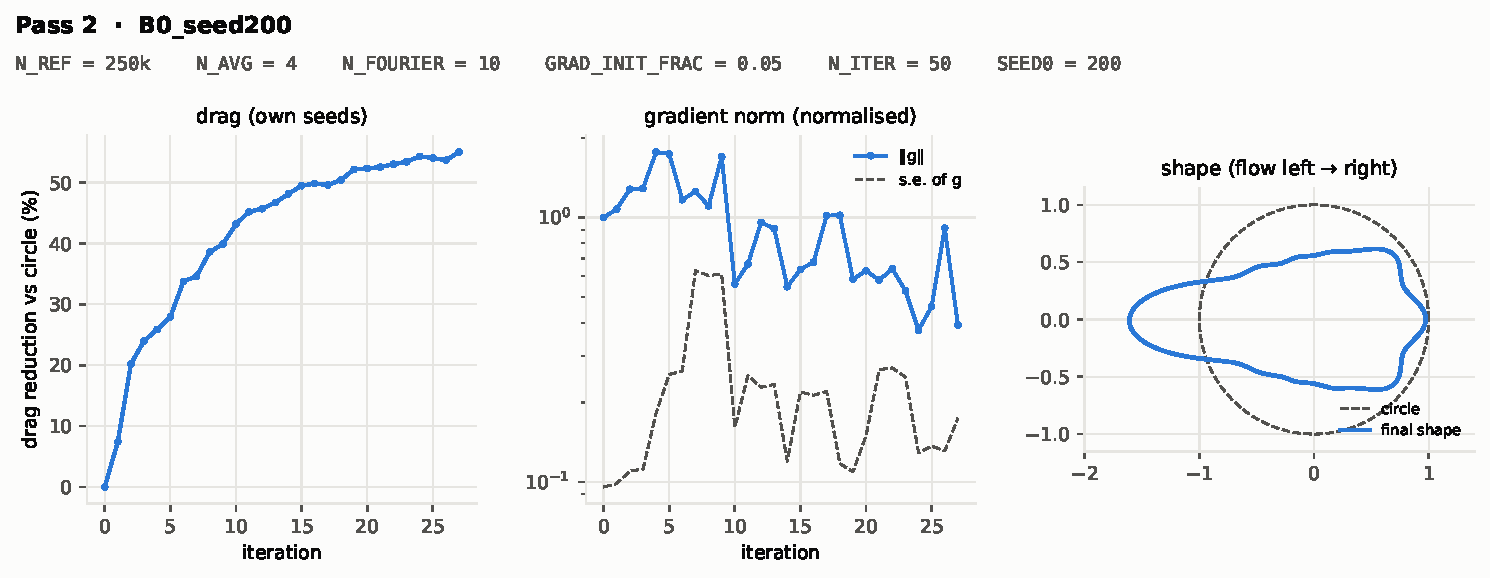
\includegraphics[width=\textwidth,height=0.42\textheight,keepaspectratio]{runs/p2_B0_seed200.pdf}\caption{Pass 2, \texttt{B0\_seed200}. The run stopped at the noise limit after 27 iterations with 4 seeds. Its drag reduction was 55.0\% relative to the circle on its own seeds and 55.4\% relative to the circle on unseen seeds. It took 0.9 hours.}\end{figure}
\begin{figure}[H]\centering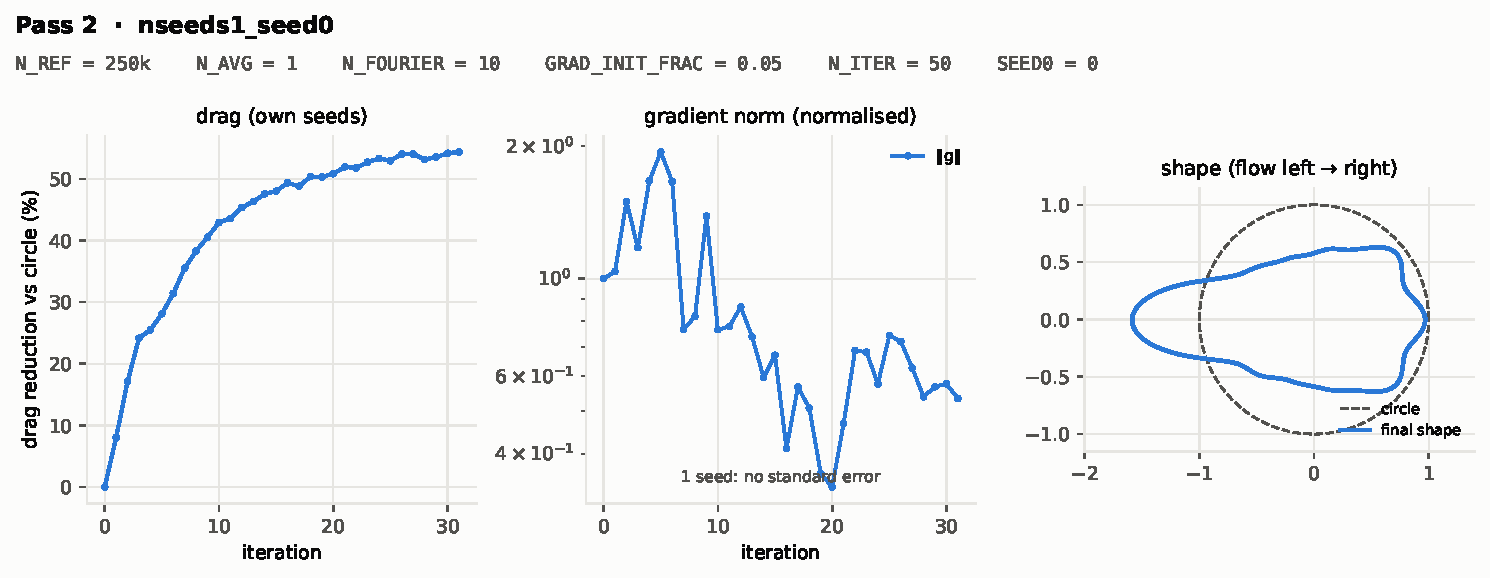
\includegraphics[width=\textwidth,height=0.42\textheight,keepaspectratio]{runs/p2_nseeds1_seed0.pdf}\caption{Pass 2, \texttt{nseeds1\_seed0}. The run stopped at the noise limit after 31 iterations with 1 seeds. Its drag reduction was 54.4\% relative to the circle on its own seeds and 53.7\% relative to the circle on unseen seeds. It took 0.9 hours.}\end{figure}
\begin{figure}[H]\centering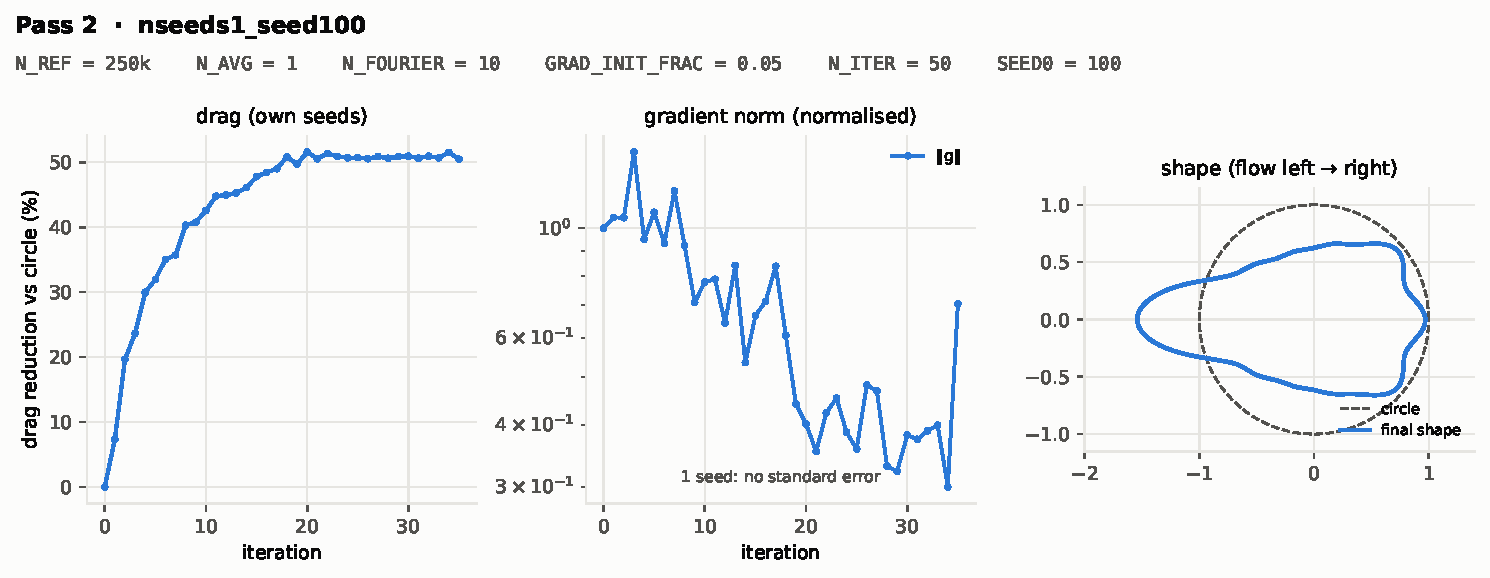
\includegraphics[width=\textwidth,height=0.42\textheight,keepaspectratio]{runs/p2_nseeds1_seed100.pdf}\caption{Pass 2, \texttt{nseeds1\_seed100}. The run stopped at the noise limit after 35 iterations with 1 seeds. Its drag reduction was 50.5\% relative to the circle on its own seeds and 51.2\% relative to the circle on unseen seeds. It took 1.0 hours.}\end{figure}
\begin{figure}[H]\centering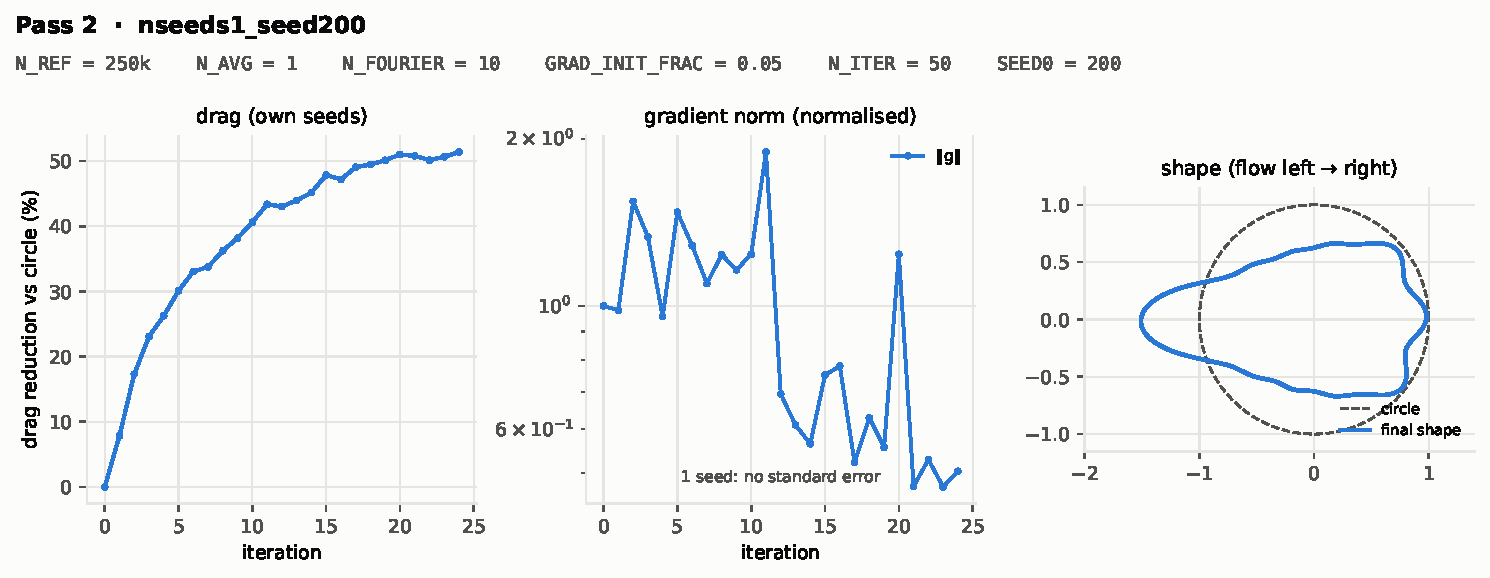
\includegraphics[width=\textwidth,height=0.42\textheight,keepaspectratio]{runs/p2_nseeds1_seed200.pdf}\caption{Pass 2, \texttt{nseeds1\_seed200}. The run stopped at the noise limit after 24 iterations with 1 seeds. Its drag reduction was 51.4\% relative to the circle on its own seeds and 50.4\% relative to the circle on unseen seeds. It took 0.8 hours.}\end{figure}
\begin{figure}[H]\centering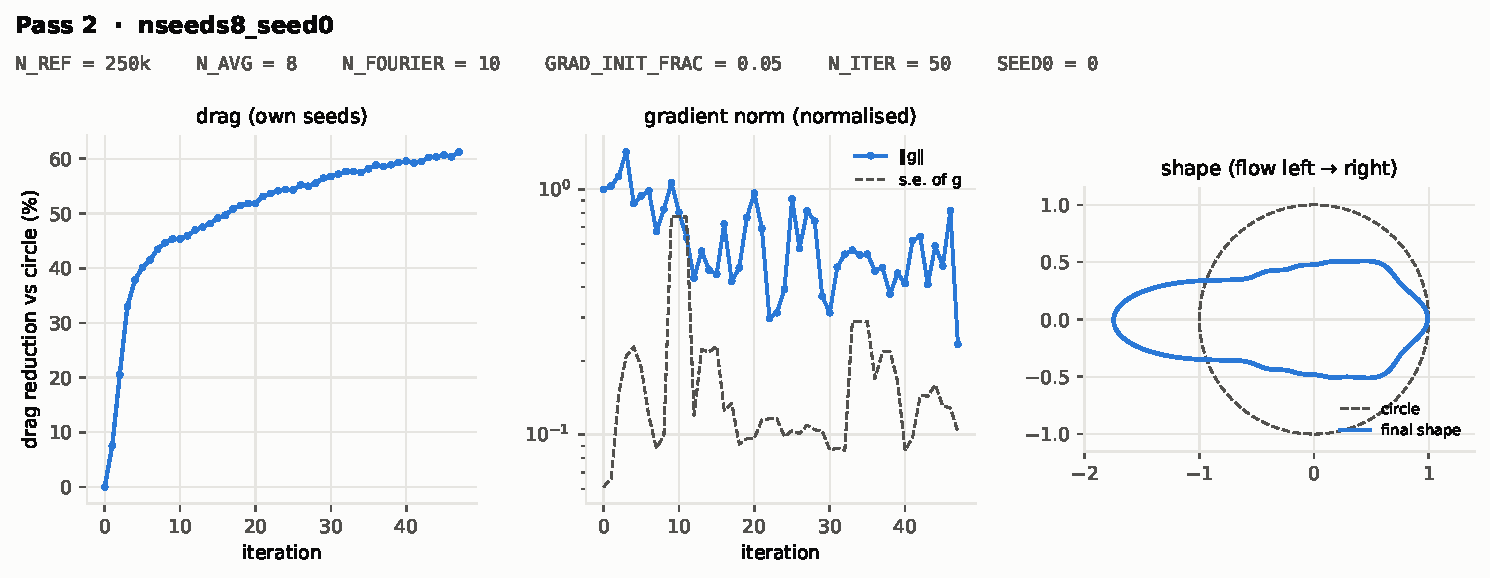
\includegraphics[width=\textwidth,height=0.42\textheight,keepaspectratio]{runs/p2_nseeds8_seed0.pdf}\caption{Pass 2, \texttt{nseeds8\_seed0}. The run stopped at the noise limit after 47 iterations with 8 seeds. Its drag reduction was 61.2\% relative to the circle on its own seeds and 61.4\% relative to the circle on unseen seeds. It took 1.5 hours.}\end{figure}
\begin{figure}[H]\centering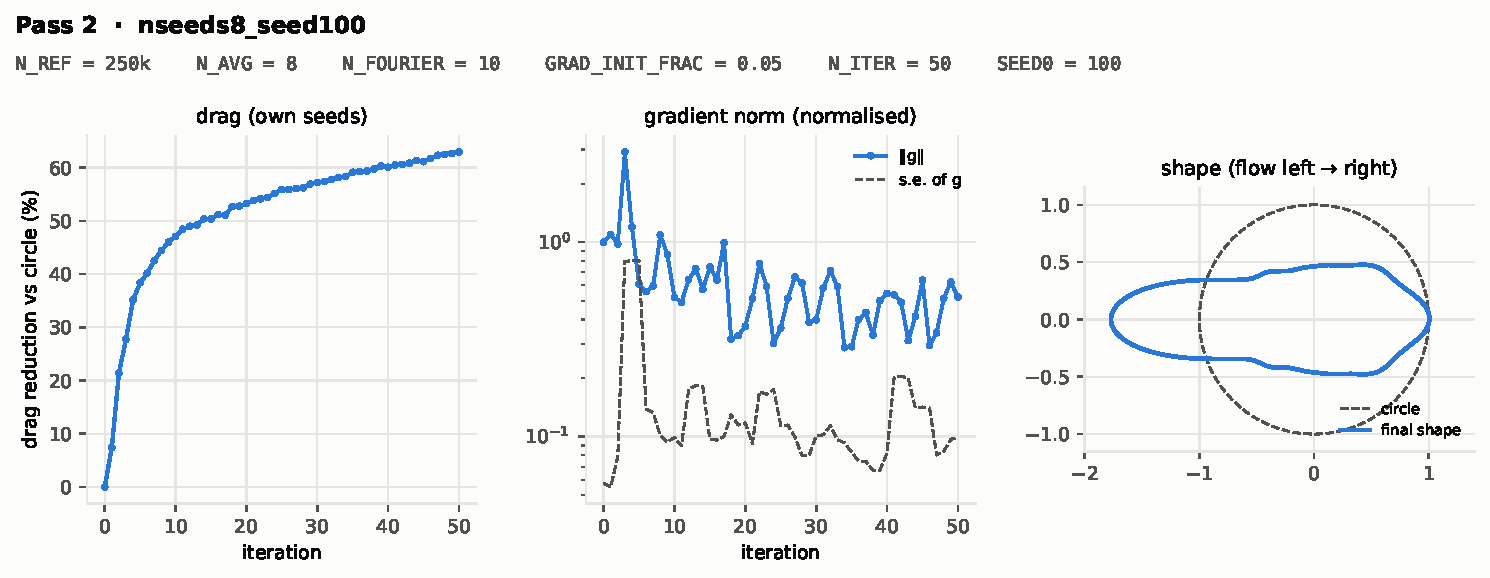
\includegraphics[width=\textwidth,height=0.42\textheight,keepaspectratio]{runs/p2_nseeds8_seed100.pdf}\caption{Pass 2, \texttt{nseeds8\_seed100}. The run stopped at the iteration limit after 50 iterations with 8 seeds. Its drag reduction was 62.9\% relative to the circle on its own seeds and 62.9\% relative to the circle on unseen seeds. It took 1.5 hours.}\end{figure}
\begin{figure}[H]\centering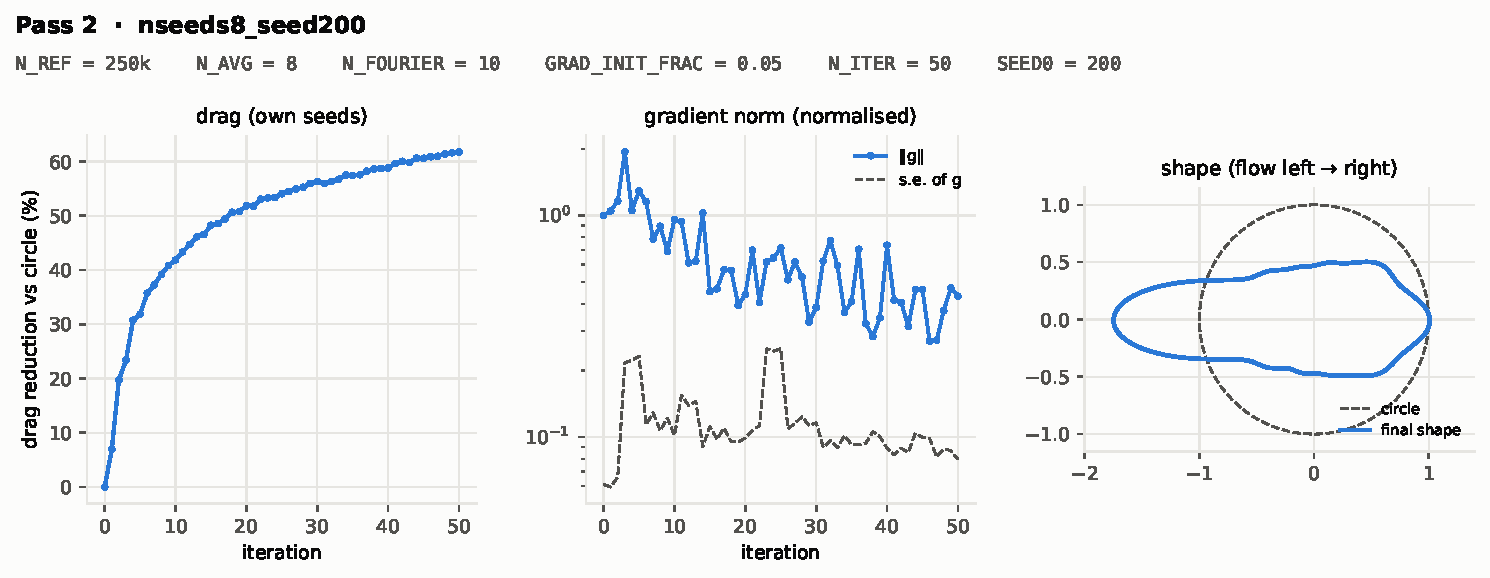
\includegraphics[width=\textwidth,height=0.42\textheight,keepaspectratio]{runs/p2_nseeds8_seed200.pdf}\caption{Pass 2, \texttt{nseeds8\_seed200}. The run stopped at the iteration limit after 50 iterations with 8 seeds. Its drag reduction was 61.7\% relative to the circle on its own seeds and 62.2\% relative to the circle on unseen seeds. It took 1.7 hours.}\end{figure}
\begin{figure}[H]\centering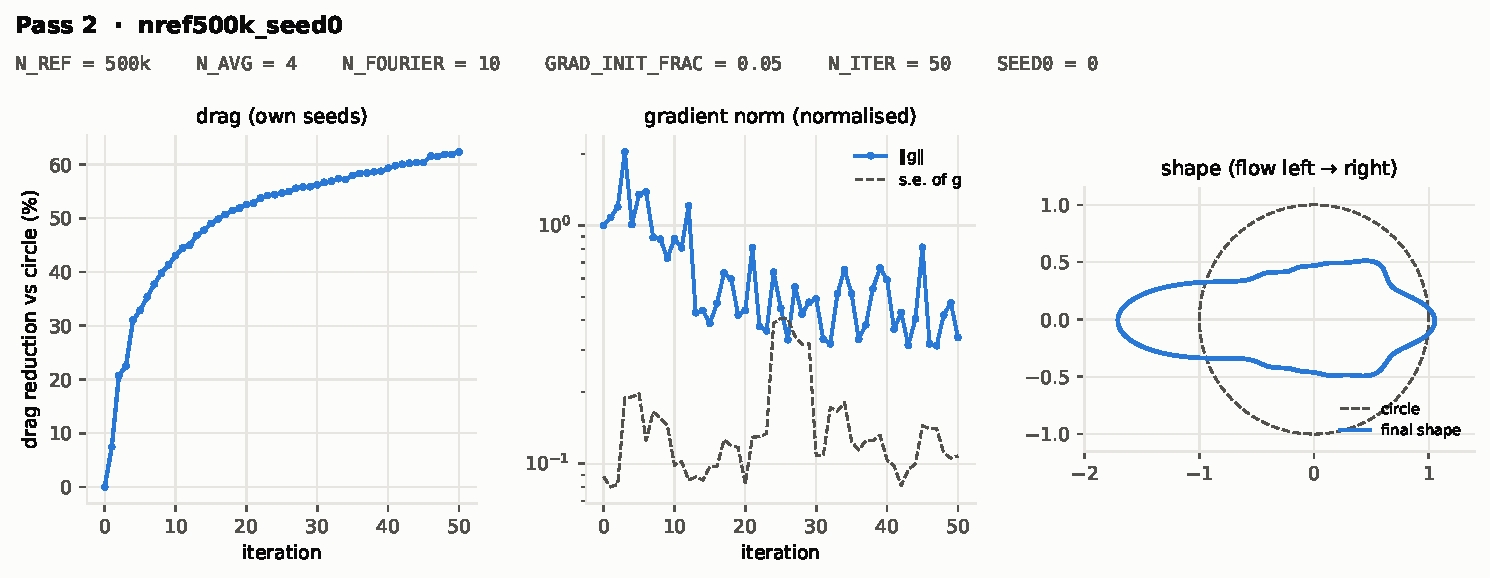
\includegraphics[width=\textwidth,height=0.42\textheight,keepaspectratio]{runs/p2_nref500k_seed0.pdf}\caption{Pass 2, \texttt{nref500k\_seed0}. The run stopped at the iteration limit after 50 iterations with 4 seeds. Its drag reduction was 62.3\% relative to the circle on its own seeds and 62.7\% relative to the circle on unseen seeds. It took 2.7 hours.}\end{figure}
\begin{figure}[H]\centering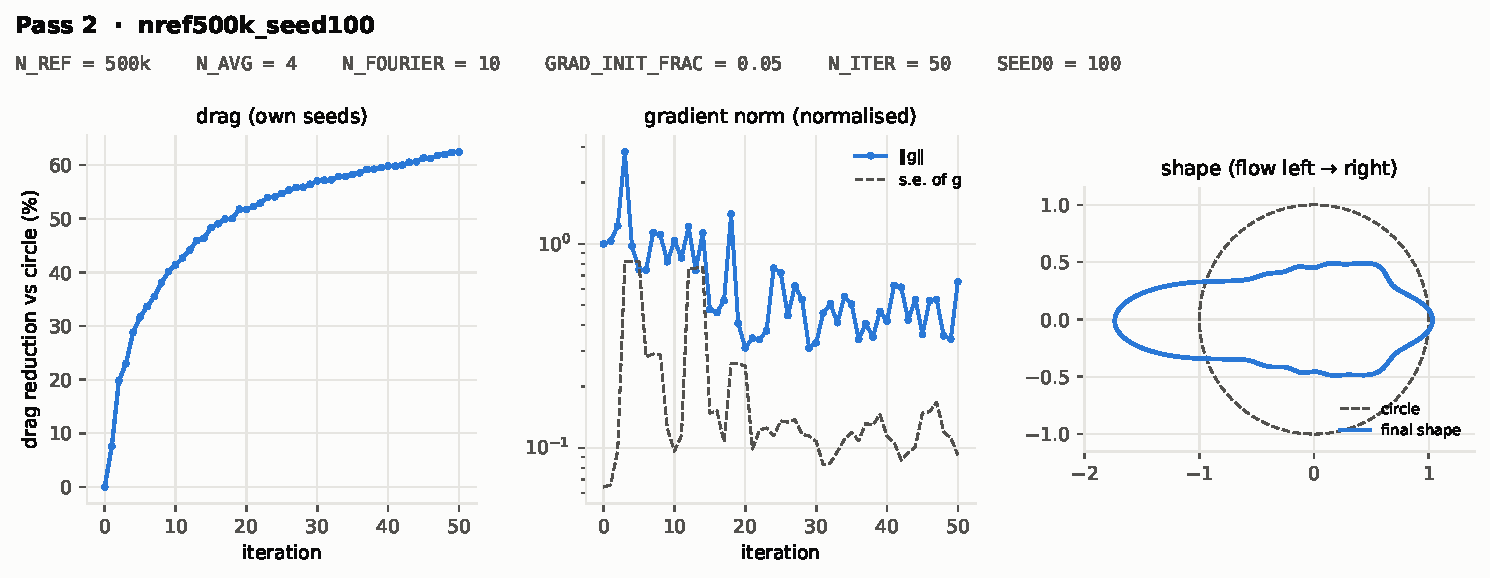
\includegraphics[width=\textwidth,height=0.42\textheight,keepaspectratio]{runs/p2_nref500k_seed100.pdf}\caption{Pass 2, \texttt{nref500k\_seed100}. The run stopped at the iteration limit after 50 iterations with 4 seeds. Its drag reduction was 62.5\% relative to the circle on its own seeds and 62.7\% relative to the circle on unseen seeds. It took 2.8 hours.}\end{figure}
\begin{figure}[H]\centering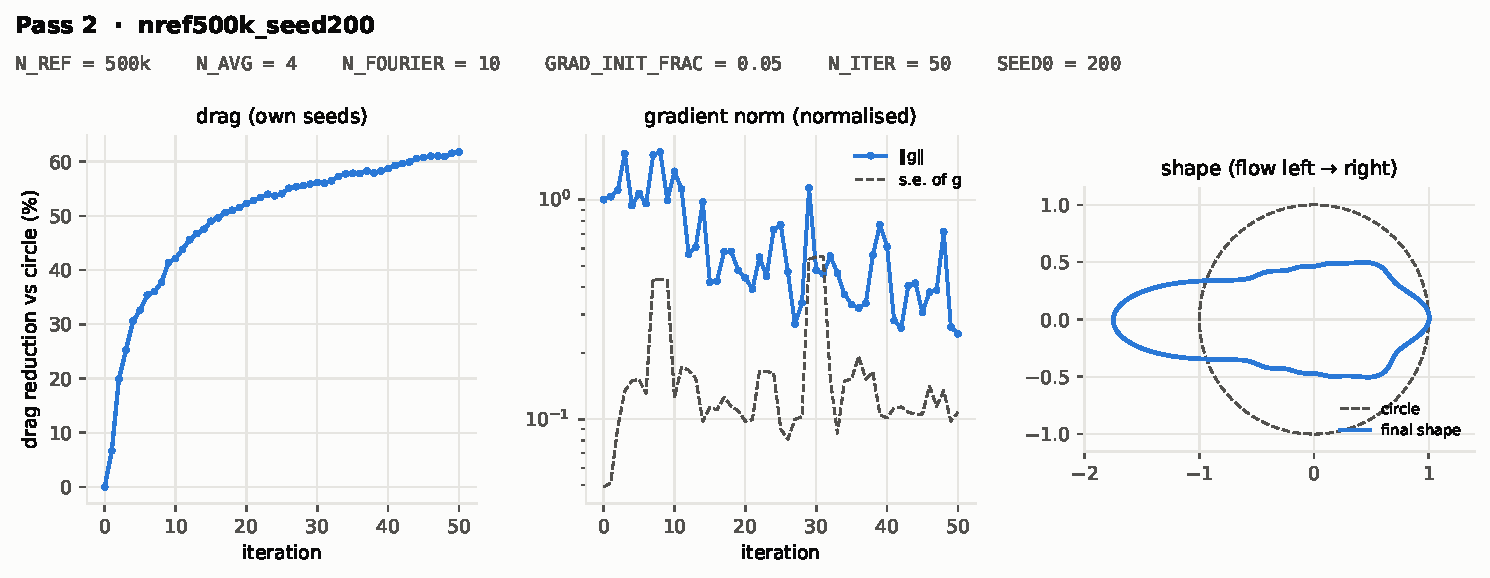
\includegraphics[width=\textwidth,height=0.42\textheight,keepaspectratio]{runs/p2_nref500k_seed200.pdf}\caption{Pass 2, \texttt{nref500k\_seed200}. The run stopped at the iteration limit after 50 iterations with 4 seeds. Its drag reduction was 61.8\% relative to the circle on its own seeds and 62.3\% relative to the circle on unseen seeds. It took 2.8 hours.}\end{figure}
\begin{figure}[H]\centering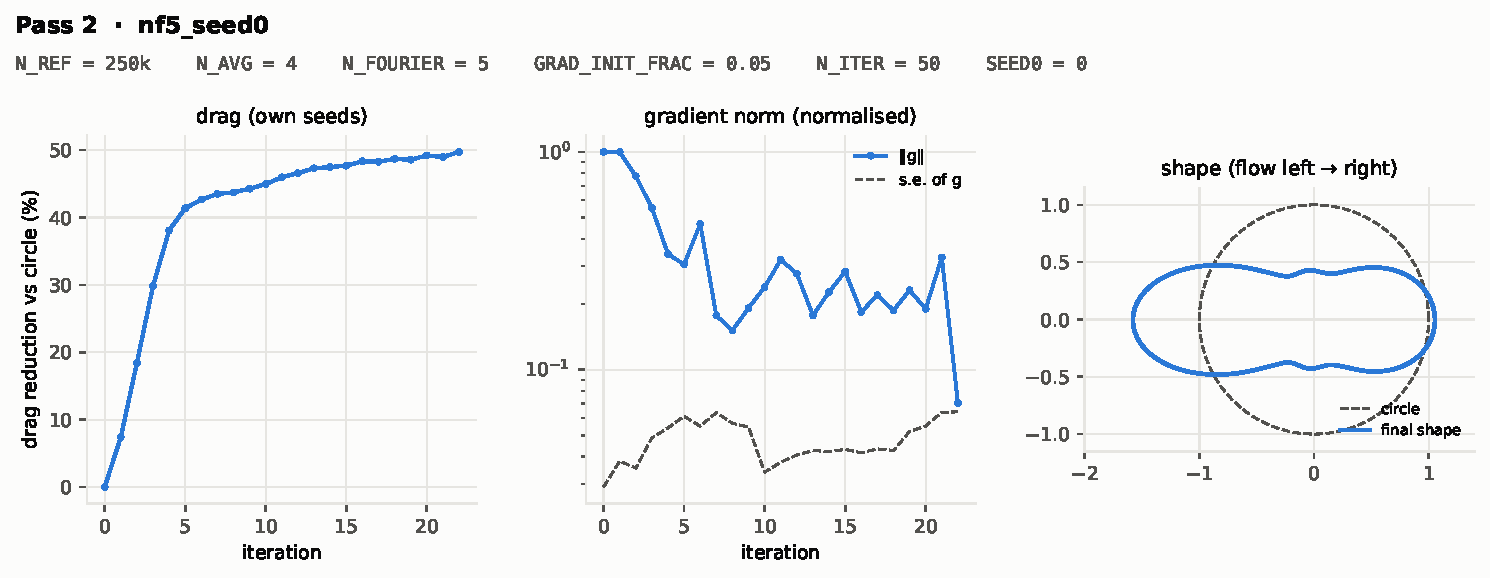
\includegraphics[width=\textwidth,height=0.42\textheight,keepaspectratio]{runs/p2_nf5_seed0.pdf}\caption{Pass 2, \texttt{nf5\_seed0}. The run stopped at the noise limit after 22 iterations with 4 seeds. Its drag reduction was 49.7\% relative to the circle on its own seeds and 49.4\% relative to the circle on unseen seeds. It took 0.6 hours.}\end{figure}
\begin{figure}[H]\centering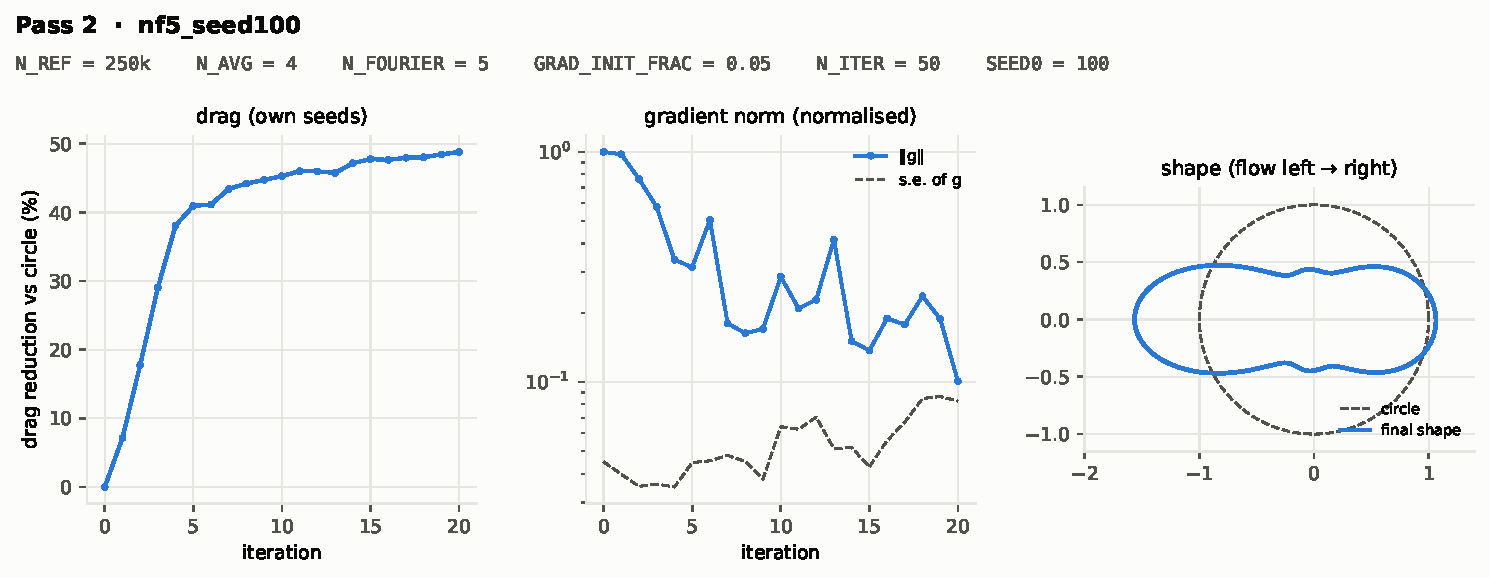
\includegraphics[width=\textwidth,height=0.42\textheight,keepaspectratio]{runs/p2_nf5_seed100.pdf}\caption{Pass 2, \texttt{nf5\_seed100}. The run stopped at the noise limit after 20 iterations with 4 seeds. Its drag reduction was 48.8\% relative to the circle on its own seeds and 49.5\% relative to the circle on unseen seeds. It took 0.4 hours.}\end{figure}
\begin{figure}[H]\centering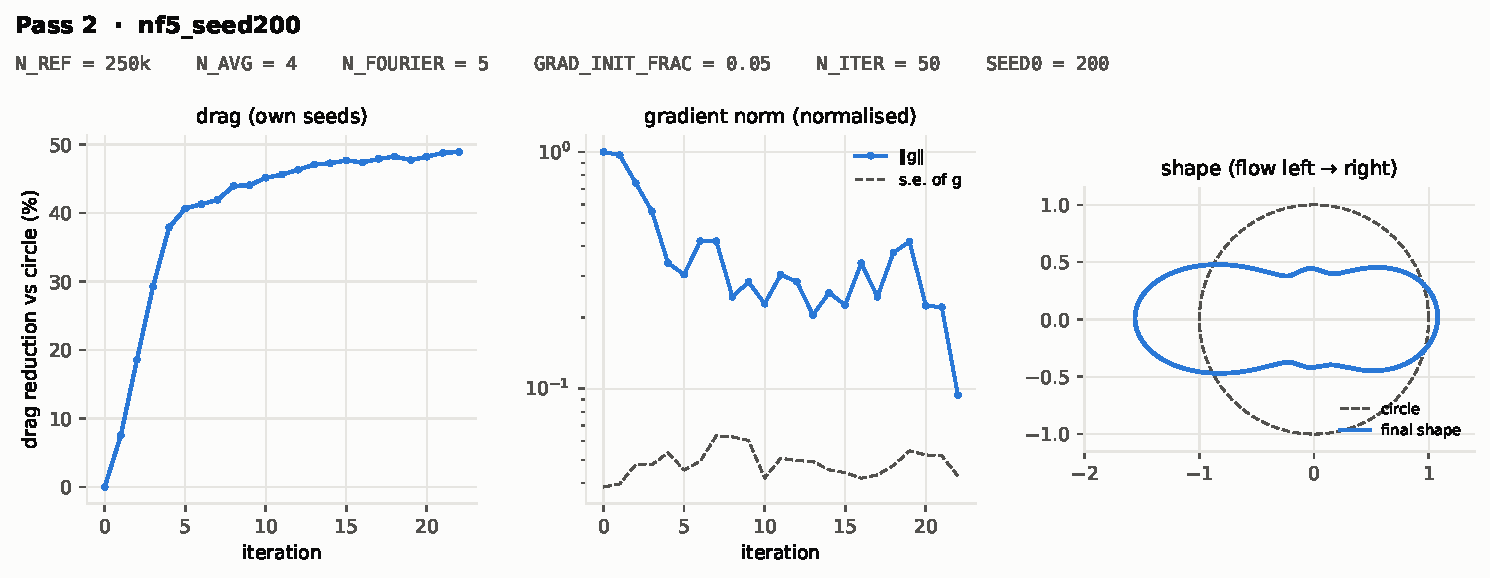
\includegraphics[width=\textwidth,height=0.42\textheight,keepaspectratio]{runs/p2_nf5_seed200.pdf}\caption{Pass 2, \texttt{nf5\_seed200}. The run stopped at the noise limit after 22 iterations with 4 seeds. Its drag reduction was 48.9\% relative to the circle on its own seeds and 49.6\% relative to the circle on unseen seeds. It took 0.4 hours.}\end{figure}
\begin{figure}[H]\centering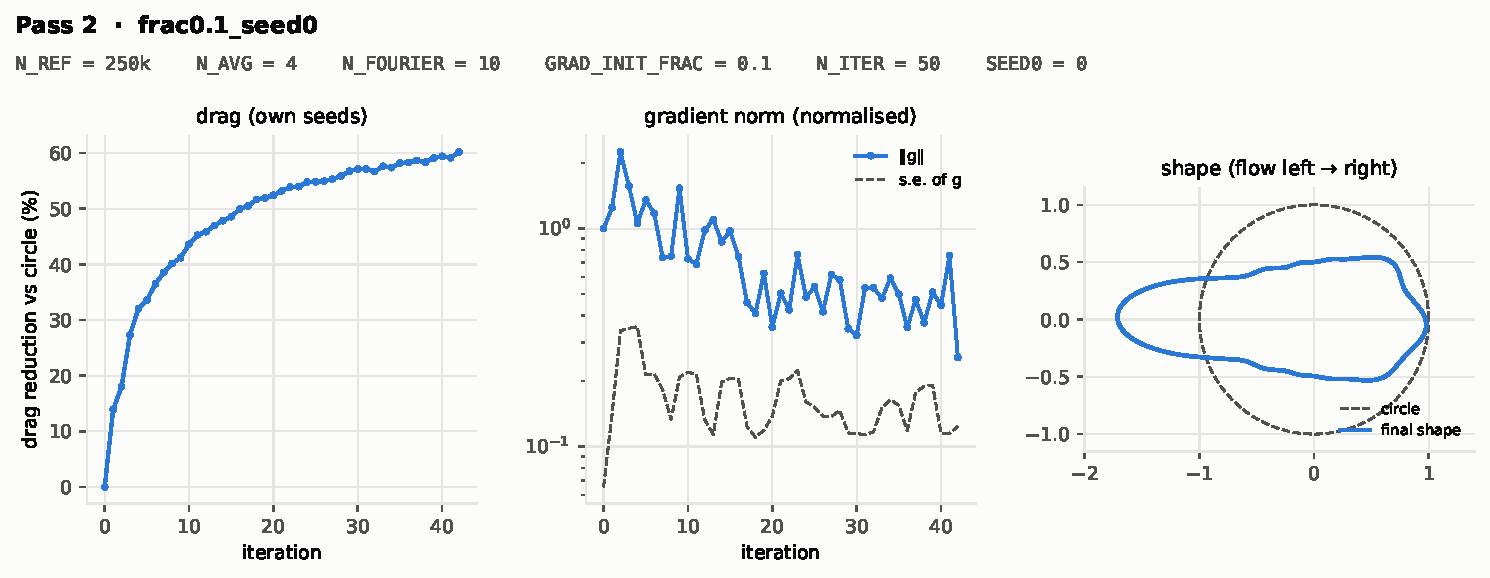
\includegraphics[width=\textwidth,height=0.42\textheight,keepaspectratio]{runs/p2_frac0.1_seed0.pdf}\caption{Pass 2, \texttt{frac0.1\_seed0}. The run stopped at the noise limit after 42 iterations with 4 seeds. Its drag reduction was 60.2\% relative to the circle on its own seeds and 60.1\% relative to the circle on unseen seeds. It took 1.3 hours.}\end{figure}
\begin{figure}[H]\centering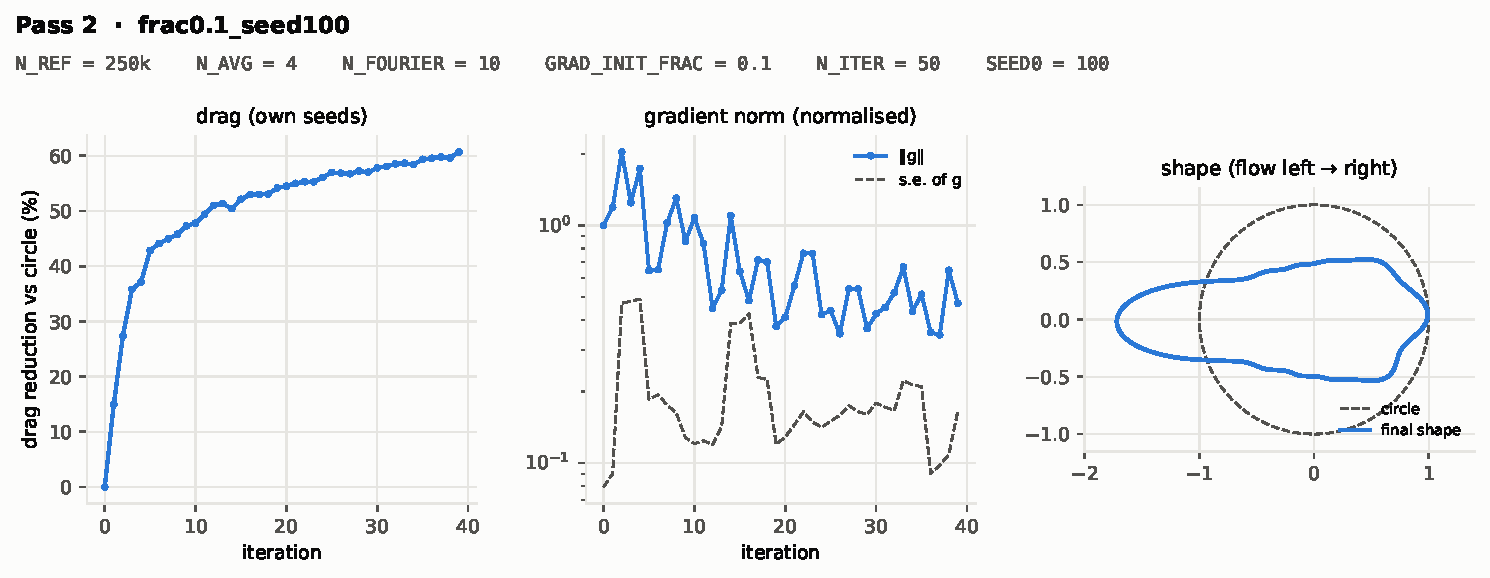
\includegraphics[width=\textwidth,height=0.42\textheight,keepaspectratio]{runs/p2_frac0.1_seed100.pdf}\caption{Pass 2, \texttt{frac0.1\_seed100}. The run stopped at the noise limit after 39 iterations with 4 seeds. Its drag reduction was 60.7\% relative to the circle on its own seeds and 60.4\% relative to the circle on unseen seeds. It took 1.2 hours.}\end{figure}
\begin{figure}[H]\centering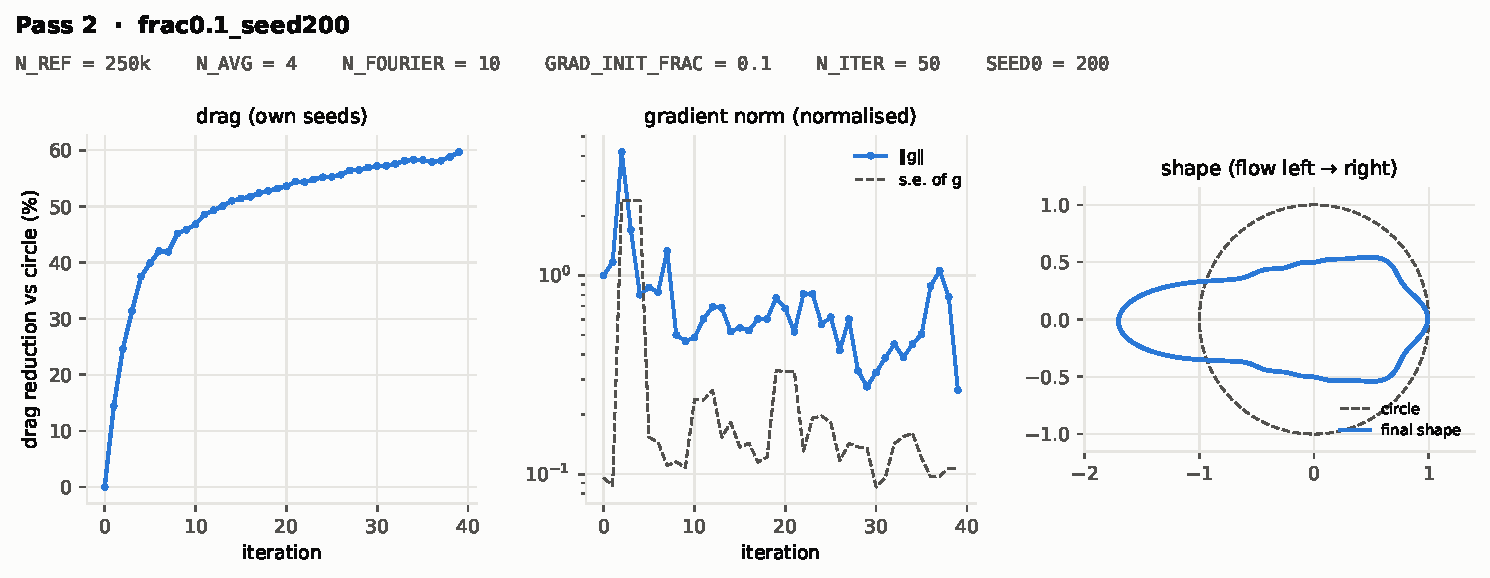
\includegraphics[width=\textwidth,height=0.42\textheight,keepaspectratio]{runs/p2_frac0.1_seed200.pdf}\caption{Pass 2, \texttt{frac0.1\_seed200}. The run stopped at the noise limit after 39 iterations with 4 seeds. Its drag reduction was 59.7\% relative to the circle on its own seeds and 59.6\% relative to the circle on unseen seeds. It took 1.2 hours.}\end{figure}
\begin{figure}[H]\centering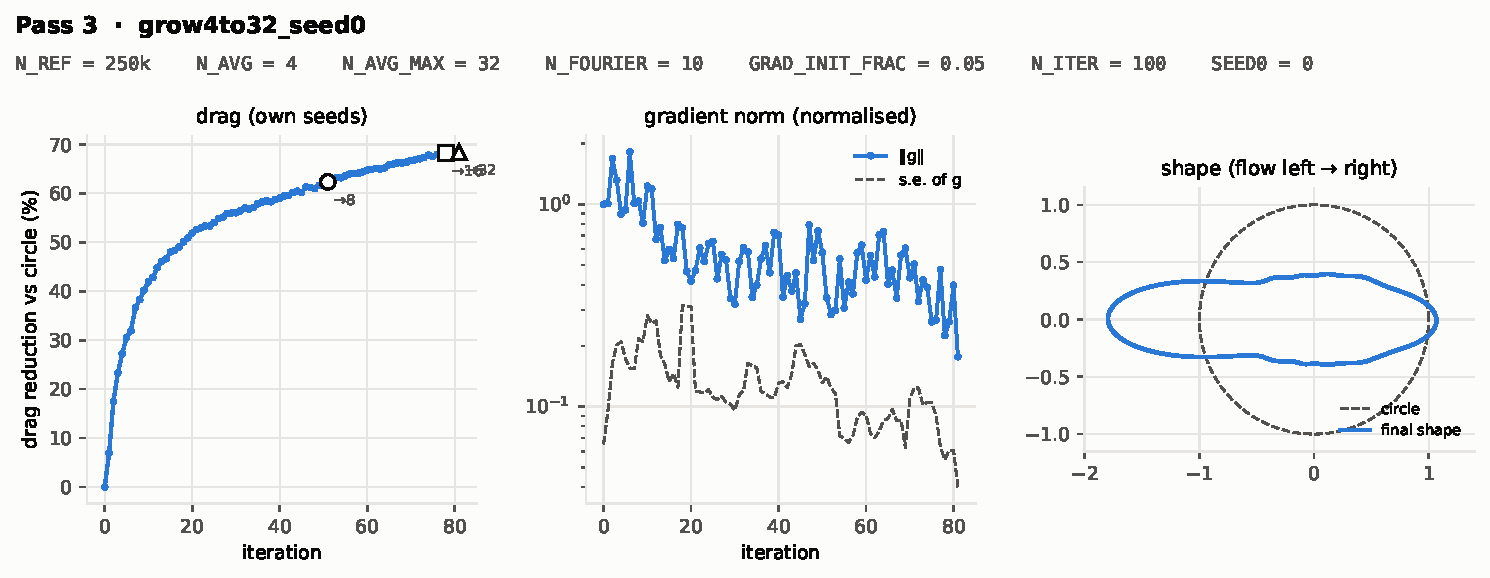
\includegraphics[width=\textwidth,height=0.42\textheight,keepaspectratio]{runs/p3_grow4to32_seed0.pdf}\caption{Pass 3, \texttt{grow4to32\_seed0}. The run stopped at the noise limit after 81 iterations with 32 seeds. Its drag reduction was 68.5\% relative to the circle on its own seeds and 68.1\% relative to the circle on unseen seeds. It took 4.1 hours.}\end{figure}
\begin{figure}[H]\centering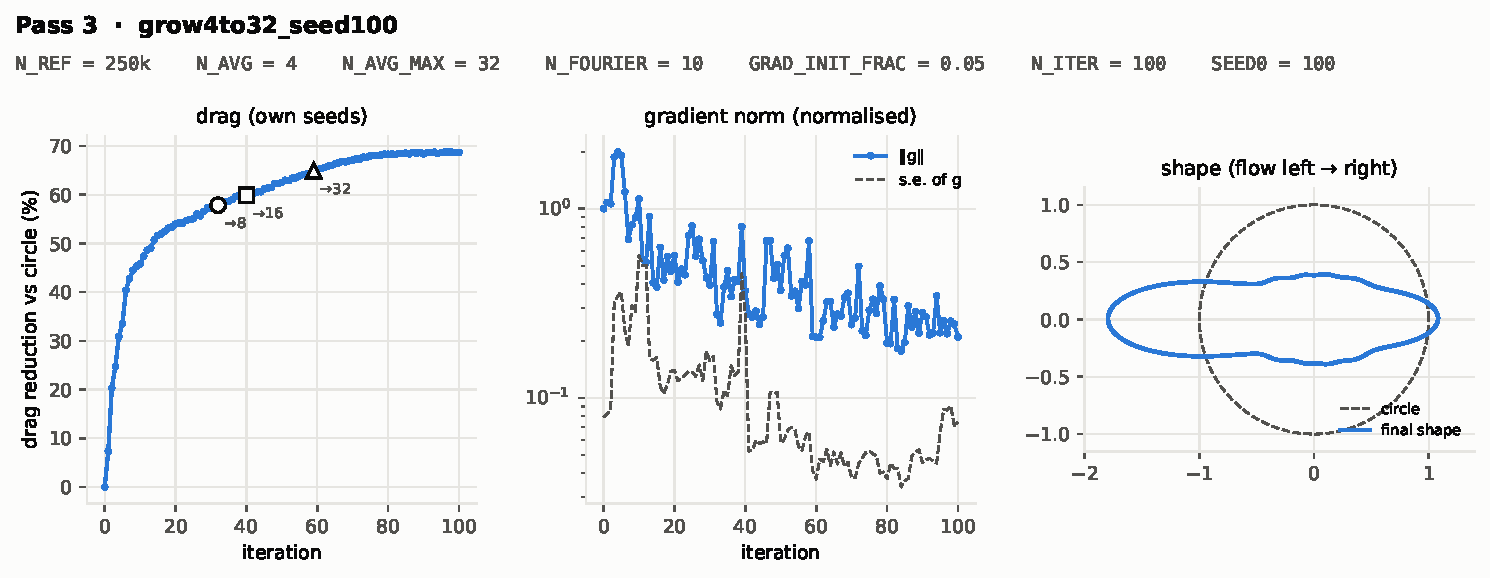
\includegraphics[width=\textwidth,height=0.42\textheight,keepaspectratio]{runs/p3_grow4to32_seed100.pdf}\caption{Pass 3, \texttt{grow4to32\_seed100}. The run stopped at the iteration limit after 100 iterations with 32 seeds. Its drag reduction was 68.7\% relative to the circle on its own seeds and 69.0\% relative to the circle on unseen seeds. It took 11.6 hours.}\end{figure}
\begin{figure}[H]\centering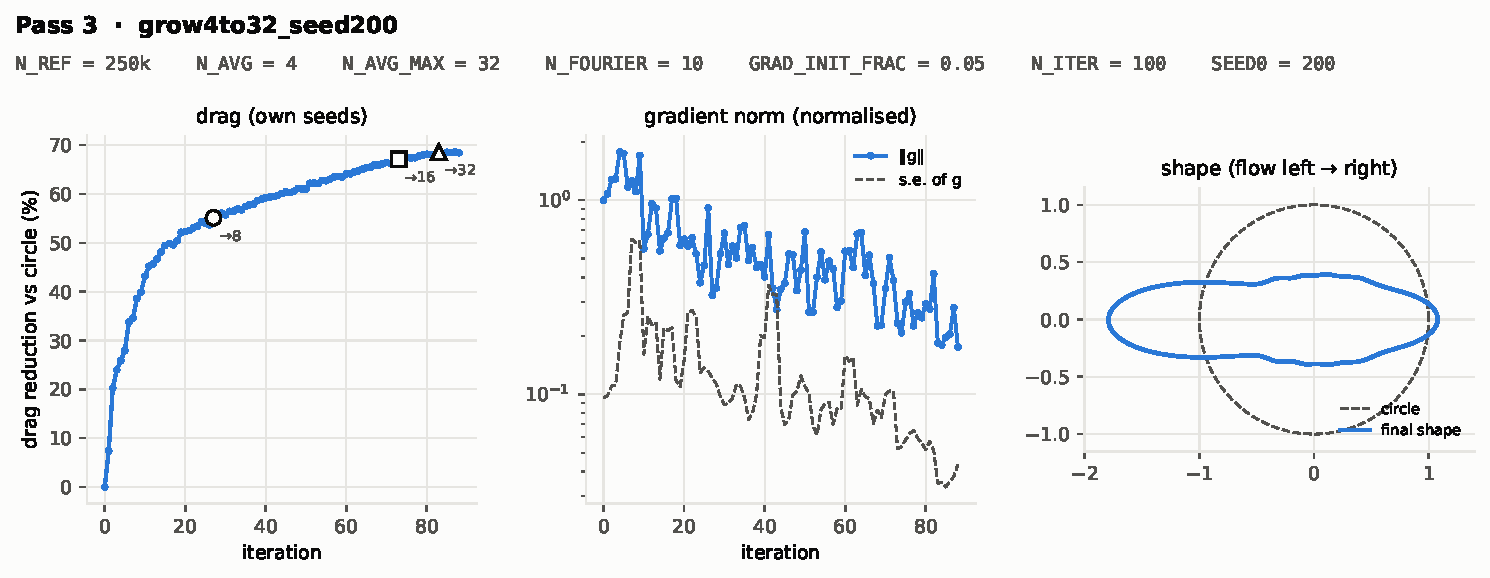
\includegraphics[width=\textwidth,height=0.42\textheight,keepaspectratio]{runs/p3_grow4to32_seed200.pdf}\caption{Pass 3, \texttt{grow4to32\_seed200}. The run stopped at the noise limit after 88 iterations with 32 seeds. Its drag reduction was 68.4\% relative to the circle on its own seeds and 68.6\% relative to the circle on unseen seeds. It took 6.1 hours.}\end{figure}
\begin{figure}[H]\centering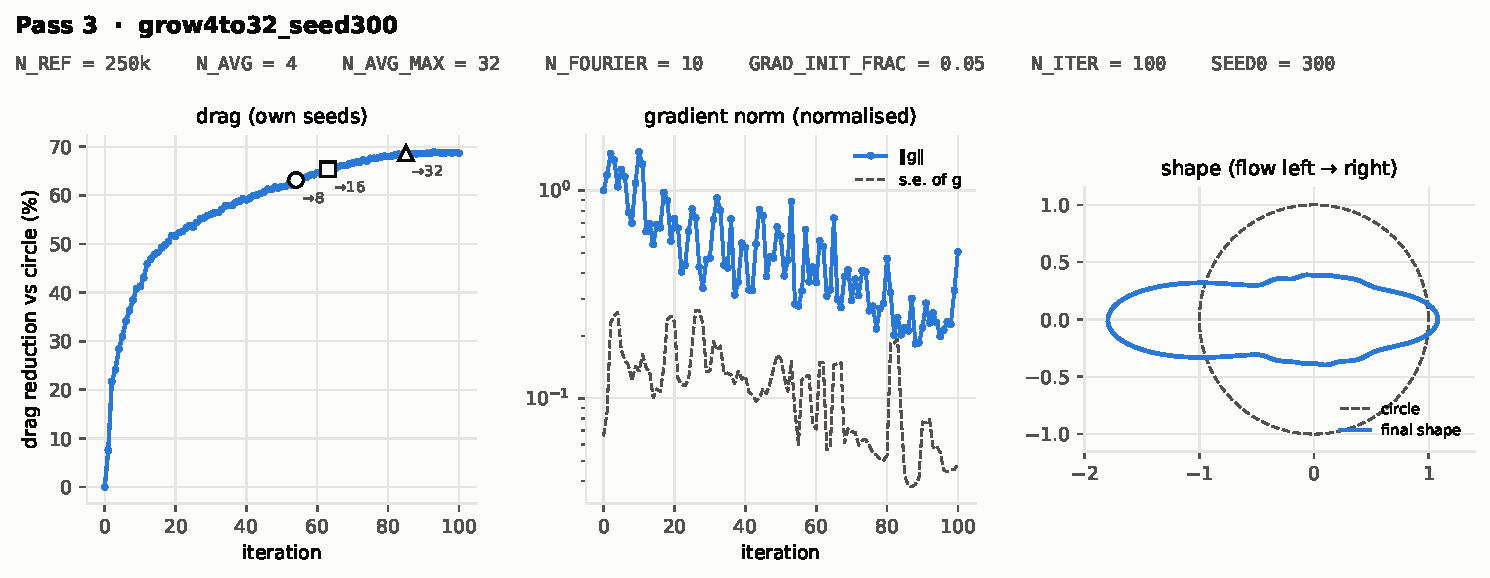
\includegraphics[width=\textwidth,height=0.42\textheight,keepaspectratio]{runs/p3_grow4to32_seed300.pdf}\caption{Pass 3, \texttt{grow4to32\_seed300}. The run stopped at the iteration limit after 100 iterations with 32 seeds. Its drag reduction was 68.7\% relative to the circle on its own seeds and 68.5\% relative to the circle on unseen seeds. It took 8.3 hours.}\end{figure}
\begin{figure}[H]\centering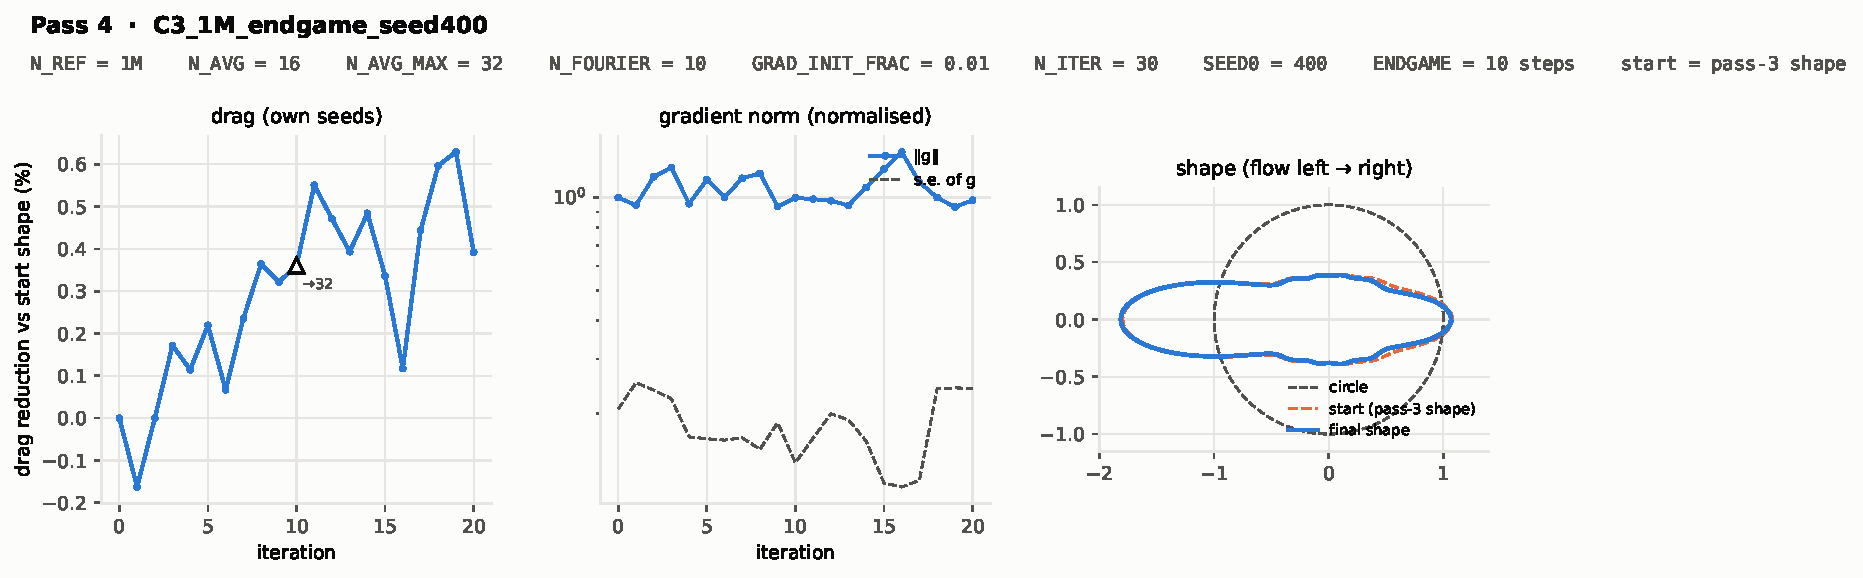
\includegraphics[width=\textwidth,height=0.42\textheight,keepaspectratio]{runs/p4_C3_1M_endgame_seed400.pdf}\caption{Pass 4, \texttt{C3\_1M\_endgame\_seed400}. The run stopped at the noise limit after 20 iterations with 32 seeds. Its drag reduction was 0.4\% relative to the start shape on its own seeds and 68.9\% relative to the circle on unseen seeds. It took 6.3 hours.}\end{figure}
\end{document}
